\documentclass[../main.tex]{subfiles}

\begin{document}

\renewcommand{\labelitemi}{\ding{226}}
\renewcommand{\labelitemii}{\ding{227}}

\part{Heavy neutrino study}

\chapter{Prospects in T2K}


In the current work we study a possibility of the improvement of the constraints on the mixing elements of the HNL in the T2K experiment. The details about the experimental setup are described~in~the~\autoref{part:T2K:general}. The main feature of the experiment for the HNL search is very intensive proton beam providing by J-PARC accelerator. The beam operation is overviewed~in~the~\autoref{ch:T2K:nu_beam}. The horn system allow to perform the analysis focusing positive or negative mesons from the proton interactions. As mentioned in the \nameref{ch:intro:HNL}, heavy neutrinos could be produced in the mesons decays. As a result there are two possible strategies of the HNL search:
\begin{itemize}
    \item measurement of the meson decay kinematics. The effect is proportional to $\left|U_l\right|^2$;
    \item search for decay products of the heavy neutrino. As both HNL production and decay are proportional to $\left|U_l\right|^2$, the final effect $\propto\left|U_l\right|^4$.
\end{itemize}

The schema of the T2K experiment is shown in~\autoref{fig:HNL:t2k_schema}. The muon monitor is the only instrument that could measure the muons directly from the meson decay. In spite of its extreme usefulness for the neutrino beam intensity and direction measurements, it could not provide necessary precision for the search of the HNL through the detection of the muons from the meson decay. Thus the only way of the heavy neutrino study in the T2K is search for the HNL decays in the near detector complex. The near detector complex (\autoref{ch:T2K:nd}) consists of on-axis INGRID detector and off-axis ND280. The most precise analysis could be done with the the ND280's time projections chambers. As we are looking for the HNL decays in the neutrino beam the gaseous detectors will observe much less background from the neutrino interactions comparing to scintillators. There are phenomenological studies~\cite{Asaka2012} that indicate the prospects of such analysis in the T2K experiment.

\begin{figure}[!ht]
    \centering
    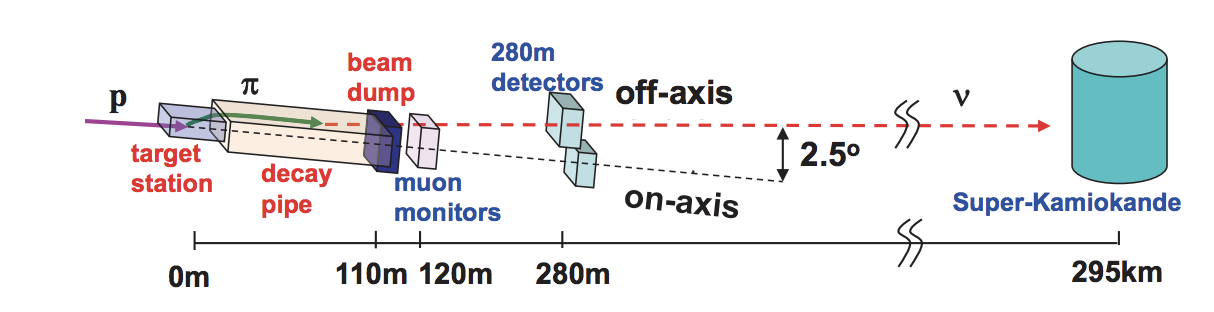
\includegraphics[width=\linewidth]{t2k_schema.png}
    \caption{A schematic view of the neutrino beamline and the detectors in the T2K experiment.}
    \label{fig:HNL:t2k_schema}
\end{figure}

With the 30 $GeV$ proton beam mainly pions are produced with some fractions of kaons. The comparison of the neutrino flux from different parent particles are presented~in~\autoref{fig:HNL:meson_flux}. As we want to study the maximum range of the HNL mass we will concentrate on the kaon decays. Thus we will be able to study the mass region up to 493 $MeV/c^2$. The overview of the HNL nature including the relation with the Standard Model particles is presented~in~\autoref{ch:intro:HNL}. The particular production and decay modes of the heavy neutrino masses that are available for the analysis in our experiment are summarized in the kinematic scheme in~\autoref{fig:HNL:mass_scale} with specific HNL mass region for each of them.

\begin{figure}[!ht]
    \centering
    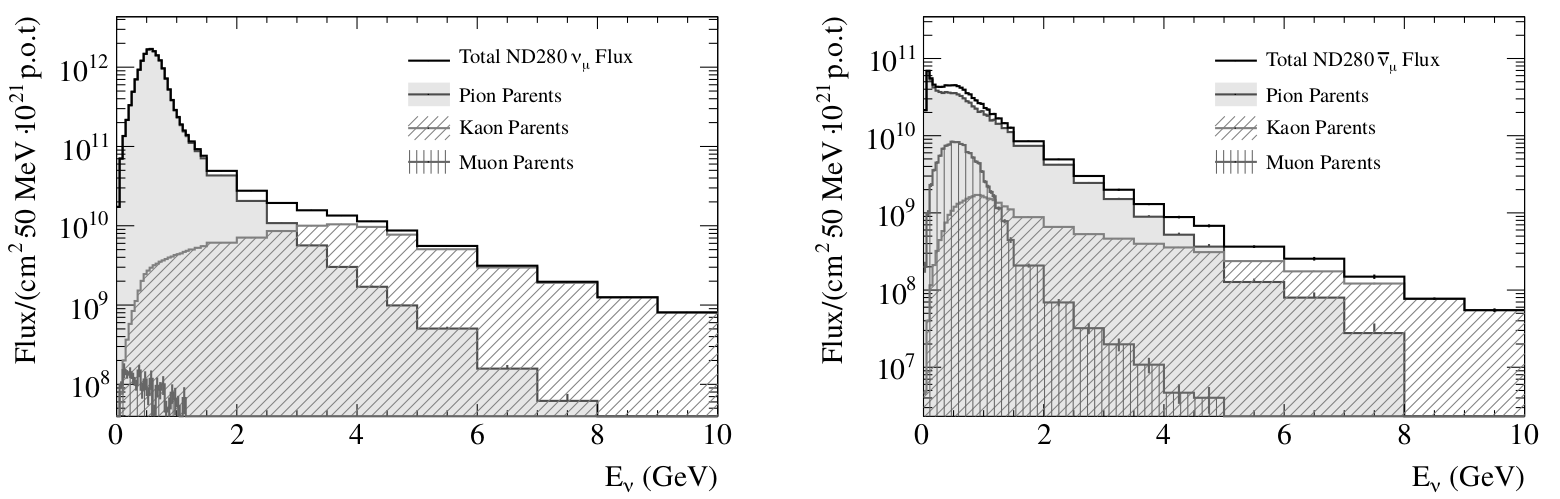
\includegraphics[width=\linewidth]{meson_flux}
    \caption{The muon neutrino and anti-neutrino flux prediction at the ND280 broken down by the neutrino parent particle type.}
    \label{fig:HNL:meson_flux}
\end{figure}

\begin{figure}[!ht]
    \centering
    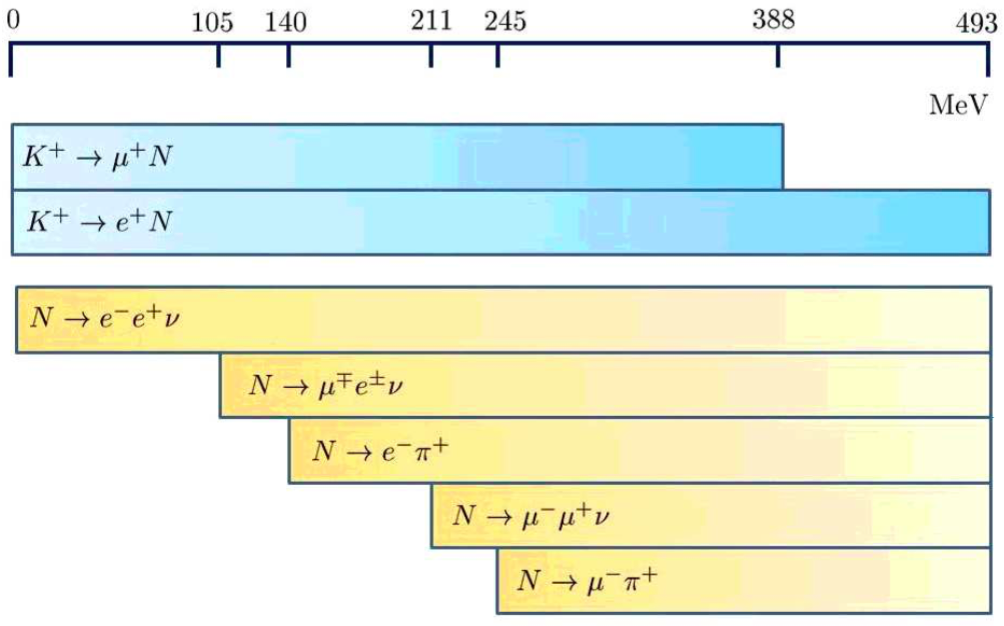
\includegraphics[width=0.7\linewidth]{HNL_mass_scale}
    \caption{Summary of the production and detection processes of the heavy neutrino available for the analysis with the ND280. The horizontal axis corresponds to the HNL mass}
    \label{fig:HNL:mass_scale}
\end{figure}

As one can see from the scheme in our study we will concentrate on the two and tree body decays of the heavy neutrino.

\begin{eqnarray}
    &N\to\ell^{\pm}\pi^{\mp} &\\
    &N\to\ell^{\pm}\ell^{\mp}\nu & \\
\end{eqnarray}

We would like to highlight the importance of the study of a HNL dimuon decay mode: $N\to\mu\mu\nu$. This decay has charge and neutral current contributions shown in Fig.~\ref{fig:DimuonFeynman} (from~\cite{Johnson1997}).

\begin{figure}[!ht]
    \begin{minipage}[!ht]{0.49\linewidth}
        \center{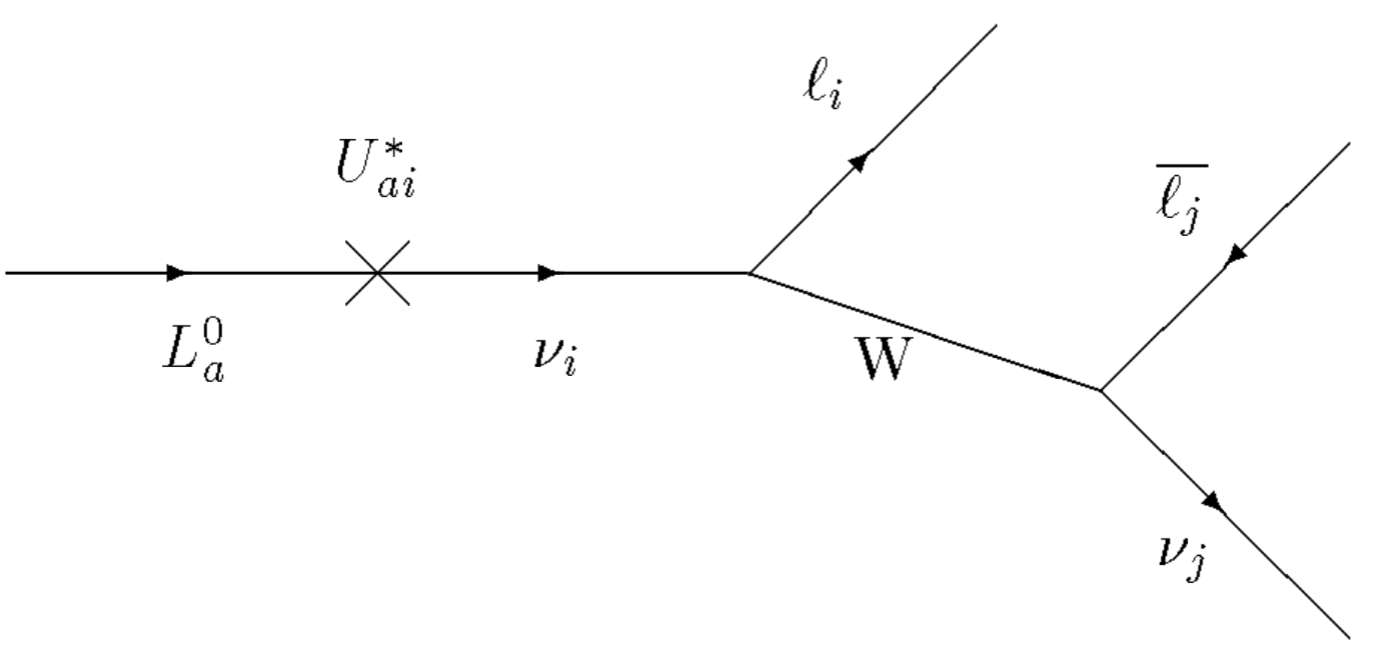
\includegraphics[width=\linewidth]{DiMuonCC.png} \\ a) }
    \end{minipage}
    \hfill
    \begin{minipage}[!ht]{0.49\linewidth}
        \center{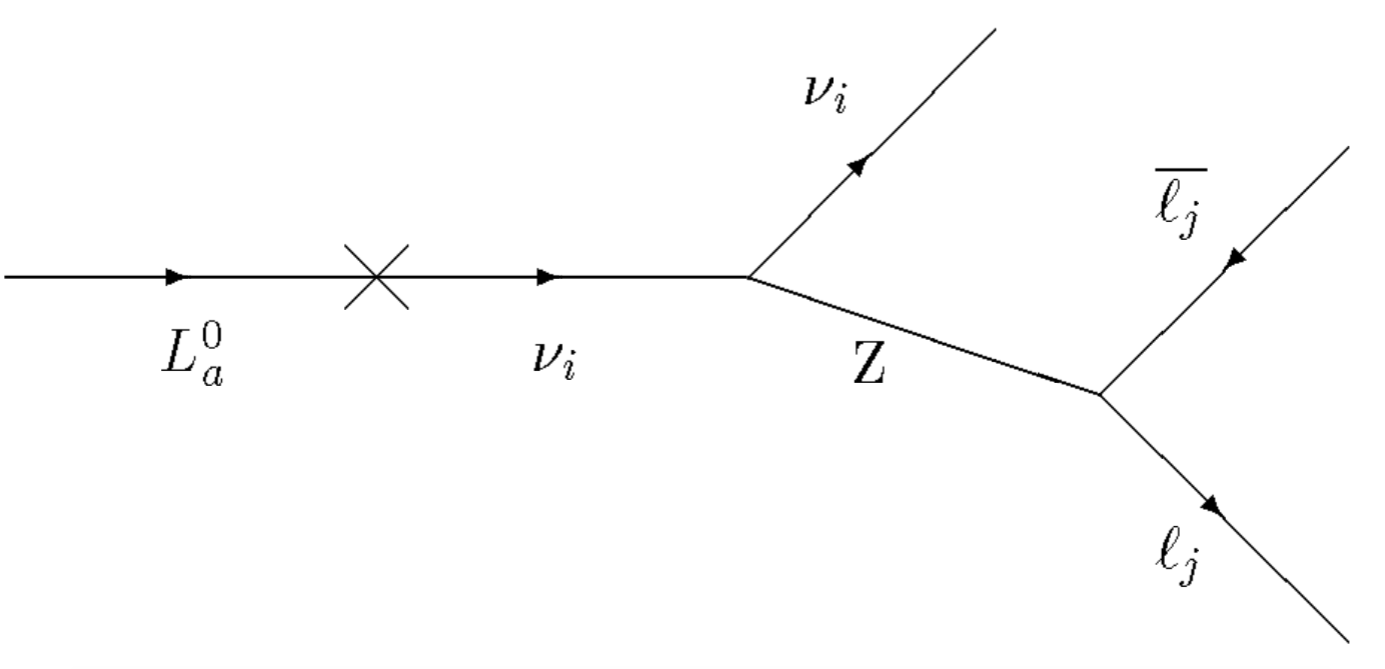
\includegraphics[width=\linewidth]{DiMuonNC.png} \\ b)}
    \end{minipage}
    \caption{Feynman diagrams for the HNL decay $N\to\mu\mu\nu$ via charged (a) and neutral (b) current.}
    \label{fig:DimuonFeynman}
\end{figure}

If the HNL decays via NC, any type of the active neutrino could be produced ($\nu_{e}, \nu_{\mu}, \nu_{\tau}$), so we can study the mixing element including $|U\tau|$. This is interesting as the upper limits on this element are rather high.

\todo{reference to the figure in intro}.

The T2K experiment uses neutrino beam from $\pi^\pm$ and $K^\pm$ decays. In our study a search of HNL from both $K^+$ and $K^-$ decays is carried out in order to increase sensitivity because of the larger statistics. We assume the Majorana nature of a HNL, this allows to study decays of $K^+$, $K^-$ and both decay modes of a heavy neutrino to $\ell^{\pm}\pi^{\mp}$.

As we focus on search of the HNL decay there are two analysis methods:
\begin{itemize}
  \item search for a peak in the HNL candidate invariant mass spectrum
  \item search for a rare event in a low background environment
\end{itemize}

The first one requires applying some simple cuts and then study difference between data and MC estimation with a peak shape. We need a rather accurate background prediction for this method. Also invariant mass resolution is one of the most important issue. We have studied the possible resolution for the HNL signal samples. The events that pass all the cuts described in the~\autoref{sec:HNL:sel} give as the reconstructed mass distribution. The examples of such distribution are presented in~\autoref{fig:HNL:InvMass}. The resolution of the invariant mass reconstruction on the HNL mass is shown in~\autoref{fig:HNL:InvMassPlot}. As one can see, RMS is quite large $\approx70MeV$. The main background processes for the HNL decay are  interactions of the active neutrinos. In near detector there are three TPCs filled with argon gas. The cross sections of the neutrino interactions in gas are not studied well. Studies of these events were performed by ArgoNeuT group~\cite{Acciarri2014}. In our momentum region ($\approx1GeV$) the uncertainties are relatively large. Other background processes can be $K^0, \Lambda, \eta$ decays, deep inelastic neutrino scattering, etc. (\autoref{sec:HNL:bg}) that are also poorly studied. Because of this we can not provide needed accuracy of the background prediction and the method of the invariant mass peak search can not be applied.
\begin{figure}[!ht]
    \begin{minipage}[!ht]{0.49\linewidth}
        \center{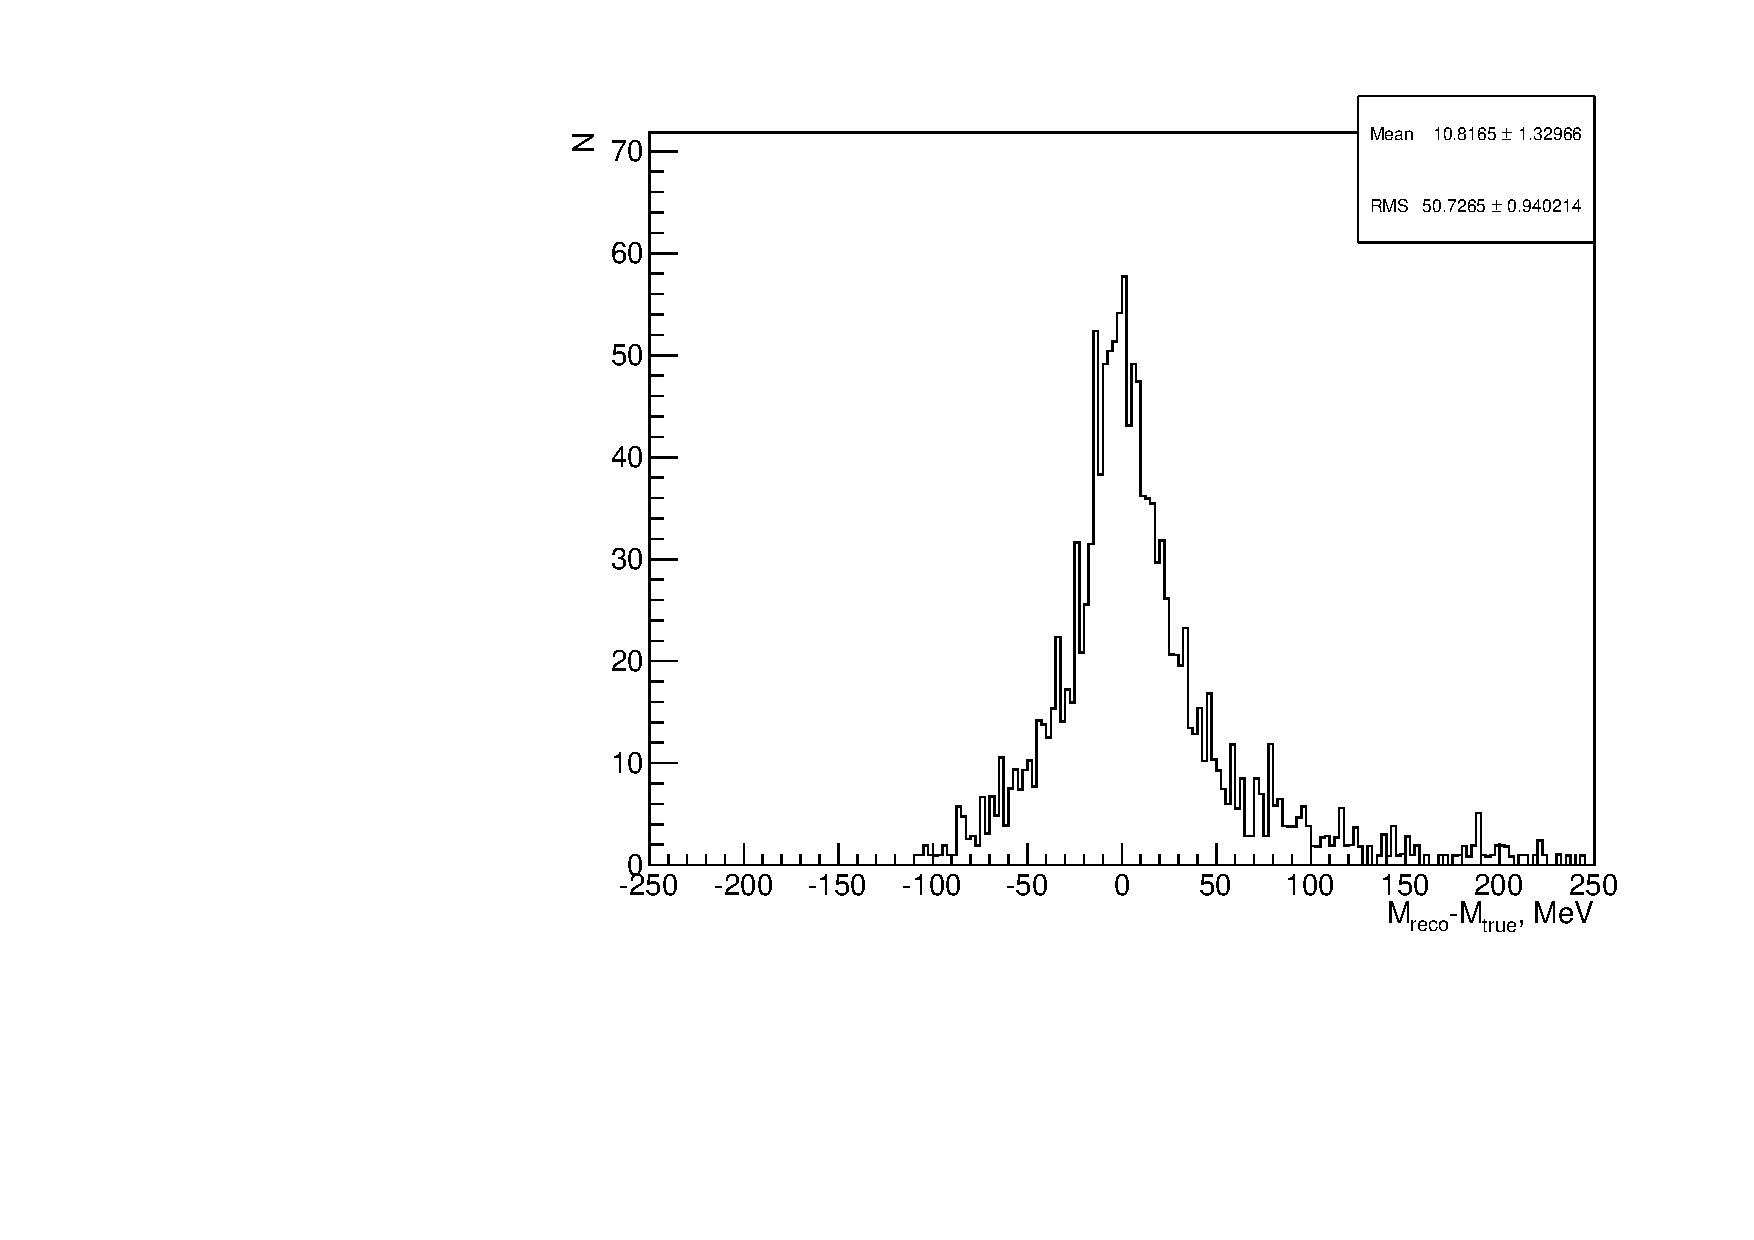
\includegraphics[width=\linewidth]{InvMass036}}
    \end{minipage}
    \hfill
    \begin{minipage}[!ht]{0.49\linewidth}
        \center{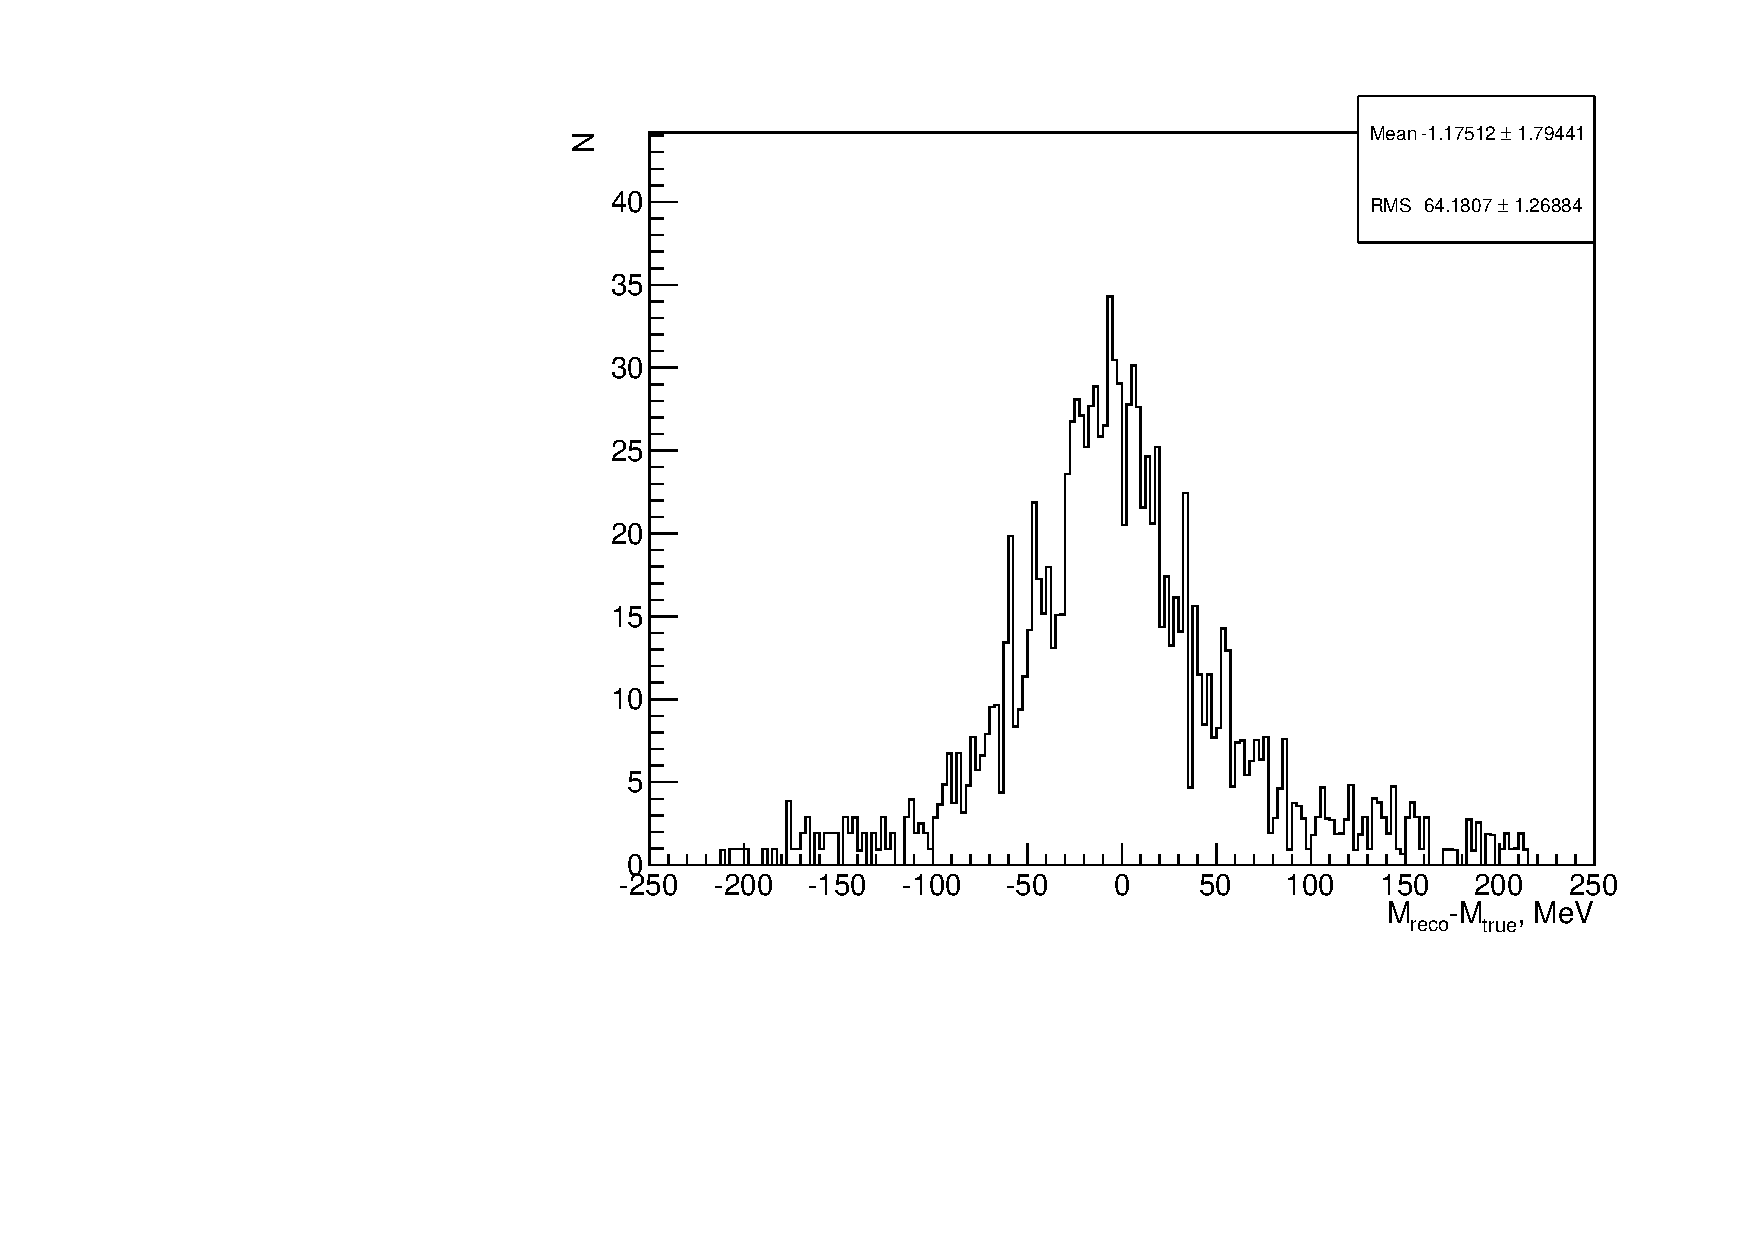
\includegraphics[width=\linewidth]{InvMass048}}
    \end{minipage}
    \caption{HNL invariant mass resolution. Left is for $M_{HNL}=360$ MeV, right is for $M_{HNL}=480$ MeV for the $\mu\pi$ mode.}
    \label{fig:HNL:InvMass}
\end{figure}

\begin{figure}[!ht]
    \begin{minipage}[!ht]{0.49\linewidth}
        \center{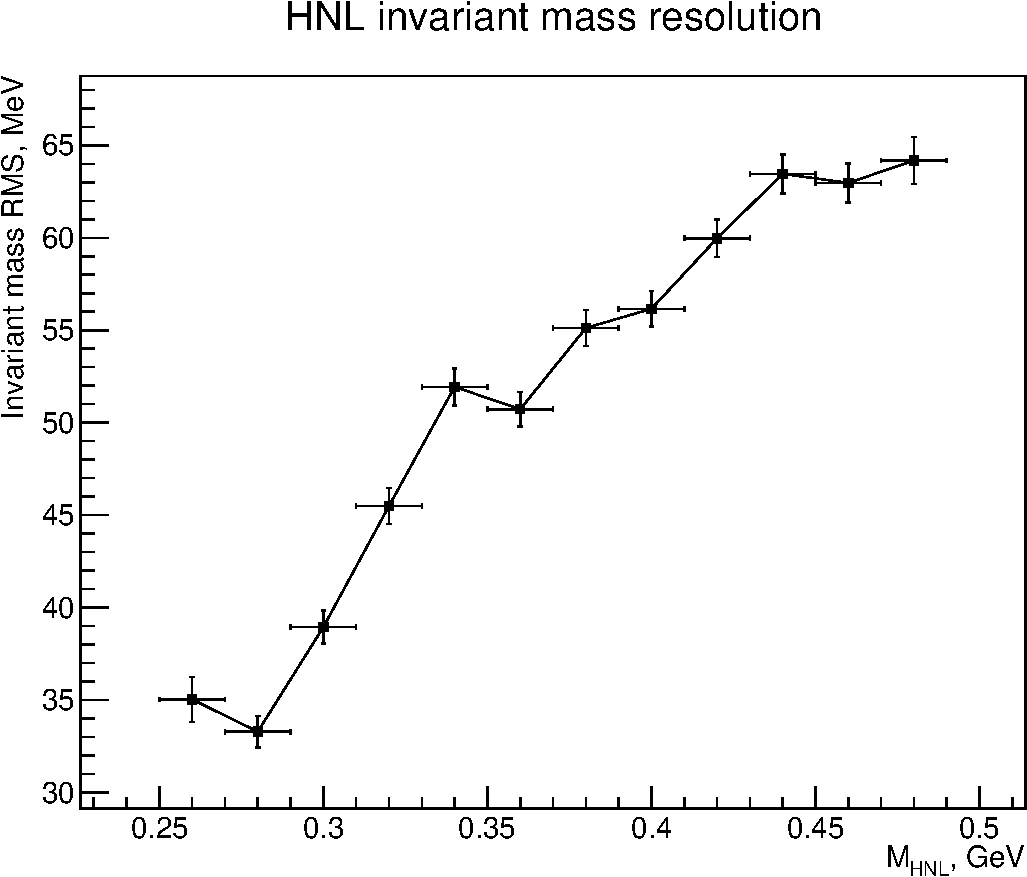
\includegraphics[width=\linewidth]{InvMassMuPlot} \\ a)}
    \end{minipage}
    \hfill
    \begin{minipage}[!ht]{0.49\linewidth}
        \center{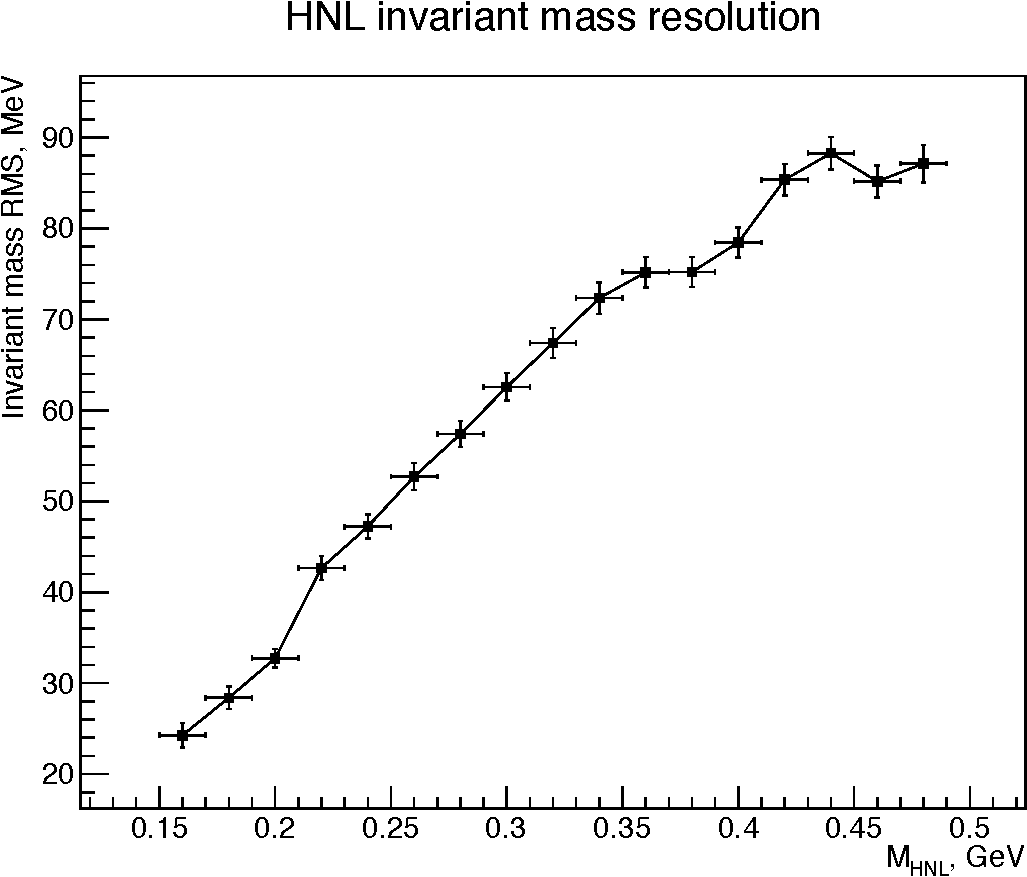
\includegraphics[width=\linewidth]{InvMassElePlot} \\ b) }
    \end{minipage}
    \caption{HNL invariant mass resolution (RMS) dependence on the HNL mass for (a) $N\to \mu\pi$ mode and (b) $N\to e\pi$ mode.}
    \label{fig:HNL:InvMassPlot}
\end{figure}

The second method requires significant background suppression. Usage of the gaseous TPC will provide very few neutrino interactions in the fiducial volume comparing to the scintillator detectors. Also the reconstruction of the heavy neutrino momentum direction could help a lot with the active neutrino events rejecting. We expect the HNL to be extremely collinear to the beam, while $\mu\pi$ pairs from the neutrino interactions will be distributed in the much wider angle. The details of the cut sequence are presented in the~\autoref{sec:HNL:sel}.

Thus we could perform a search of a few signal events in an extremely low background environment ($\approx1$). The details of the used statistical approach could be found in~\autoref{sec:HNL:stat}.

\chapter{HNL flux simulations}
\label{ch:HNL:HNLsim}

First of all we need to estimate the sensitivity to the mixing elements in our experiment. So we need to evaluate the HNL flux at the ND280. We decided to use the results of the neutrino flux simulation that was developed for the oscillation analysis within the T2K experiment. With this simulation we have all the information about the neutrinos entering the ND280 and their parent particles. Because of the kinematics the phase space of the meson decay into HNL is more limited then the decay into massless neutrino. E.g. the maximum angle of the HNL direction with respect to the parent meson direction is lower comparing to the massless neutrino case. Thus if we consider only mesons that could produce neutrino entering ND280 and omit all the others, we will definitely take all the possible HNL parent particles.

For the heavy neutrino simulation we take the particular meson decay and reweight is taking into account new kinematic and the branching ratios. Thus we will obtain the heavy neutrino spectrum in our detector.

\section{T2K flux simulation}
The accurate prediction of the neutrino flux is extremely important for the precise oscillation analysis. That's why the T2K collaboration have spent great effort on tuning the flux simulation in the most accurate way~\cite{Abe2013}. All the elements of the neutrino beamline (\autoref{ch:T2K:nu_beam}) are taken into account. The most tricky part is the evaluation of the meson production through the proton interactions in the carbon target. To reduce the systematic uncertainties the measurements from the NA61/SHINE experiment are used~\cite{Collaboration2018}.

\todo{details about NA61}.

The flow diagram of the neutrino flux simulation is shown in~\autoref{fig:HNL:nu_flux_sim}.

\begin{figure}[!ht]
    \centering
    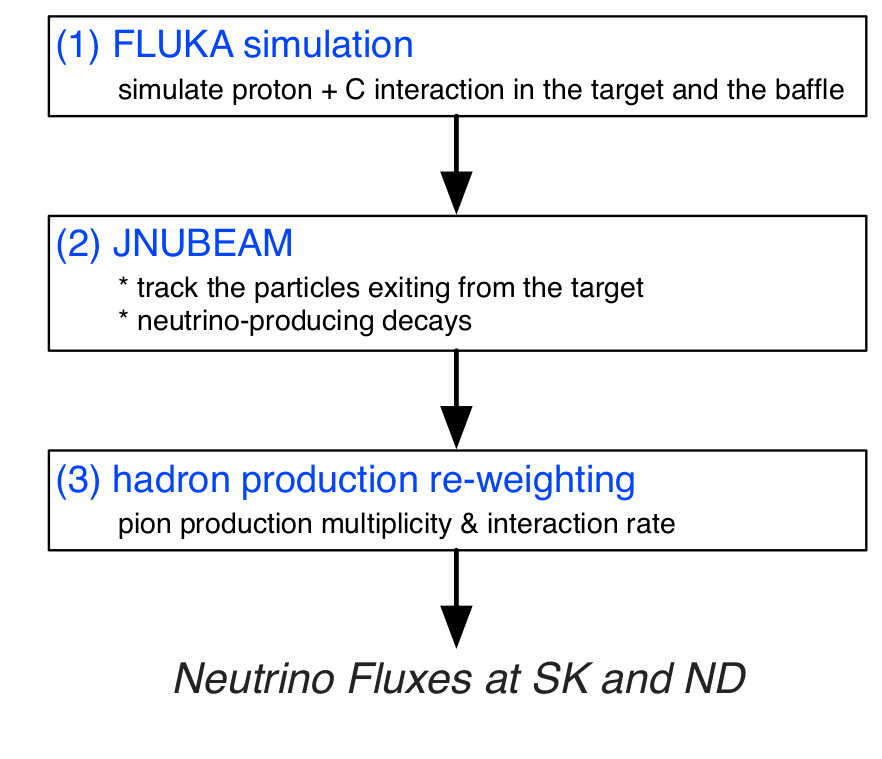
\includegraphics[width=0.5\linewidth]{nu_flux_sim}
    \caption{The neutrino flux prediction flow}
    \label{fig:HNL:nu_flux_sim}
\end{figure}

The proton beam spatial distribution and divergence are measured in the beamline monitors. The FLUKA generator is used to perform the simulation of the hadron interaction with the target and a buffle. Incident protons are set at known position and with kinetic energy of 30 GeV. The information of the generated particles that exited the simulated volume it stored. The next step is a JNUBEAM generator that takes the information about the particles from the previous step and tracks them through the horns and helium vessel, decay volume and surrounding concrete until the decay or the kinetic energy drop down below the threshold (10 MeV). At this step $\pi^\pm$, $K^\pm$, $K_L^0$ and $\mu^\pm$ decays are considered as neutrino sources. In order to save the computing time, the daughter neutrino is pointing towards the detector plane and the appropriate kinematic weight is assigned to the event.


After such simulation chain is performed and the outgoing neutrino is saved the hadronic chain in each event is reweighted based on the hadron interaction measurements. In our studies we are particularly interested in the kaon production. The generated kaon phase space and the coverage of the NA61 measurements are presented in~\autoref{fig:HNL:kaon_ps}.

After the reweighing of the hadron chains the total accuracy of the prediction is evaluated. The main systematic errors come from the hadronic interactions, primary beam alignment, horn current and magnetic field. The resulting uncertainty of the neutrino flux predictions are shown in~\autoref{fig:HNL:nu_flux_uncert}.

\begin{figure}[!ht]
    \begin{minipage}[!ht]{0.49\linewidth}
        \centering
        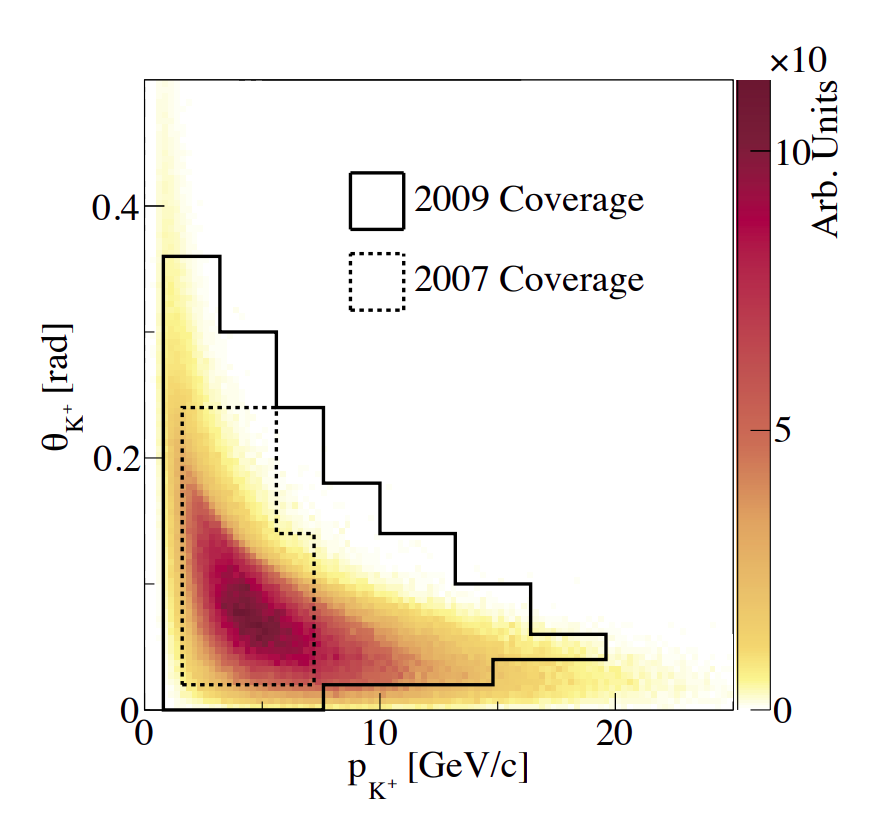
\includegraphics[width=\linewidth]{nu_flux_kaons}
        \caption{The phase space of positive kaons contributing to the predicted neutrino flux and the regions covered by the NA61/SHINE.}
        \label{fig:HNL:kaon_ps}
    \end{minipage}
    \hfill
    \begin{minipage}[!ht]{0.49\linewidth}
        \centering
        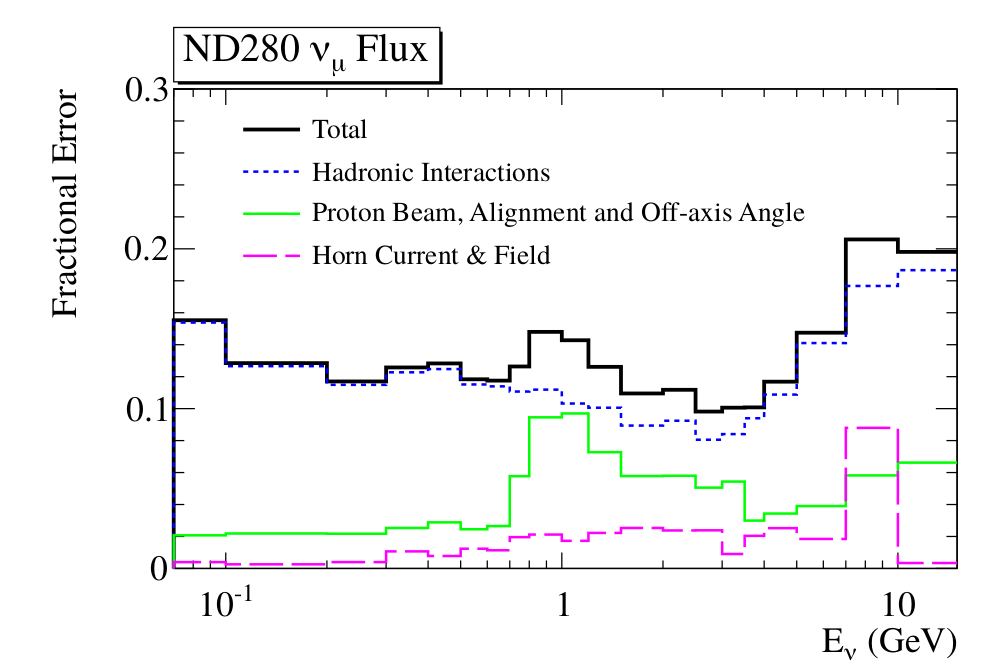
\includegraphics[width=\linewidth]{nu_flux_uncert}
        \caption{Fractional errors for the neutrino (left) and anti-neutrino (right).}
        \label{fig:HNL:nu_flux_uncert}
    \end{minipage}
\end{figure}


\section{HNL production}

For the propose of our study we would like to reweight the kaons decays based on the new kinematics and branching ratios. But we want to keep all the fine-tuning described in the previous section in order to keep the uncertainties as small as possible. Looking at the~\autoref{fig:HNL:nu_flux_sim}, we would like to change ``(2) JNUBEAM: neutrino-producing decays'', but to keep everything else at place.

Every neutrino event in original files has a weight, which was calculated as
\begin{equation}
    weight_{K\mu2}=scale_{POT}\cdot weight_{geom}\cdot P_{save}^{-1}\cdot Br_{K\mu2},
\end{equation}
where
\begin{itemize}
    \item $scale_{POT}$ --- $10^{21}$ POT normalization;
    \item $weight_{geom}$ --- probability of neutrino getting to the certain point of the detector plane, which was selected randomly;
    \item$P_{save}^{-1}$ --- probability to save event, in order to have results of MC model in a wide spectrum;
    \item $Br_{K\mu2}$ --- branching of $K\rightarrow\mu\nu_{\mu}$ decay.
\end{itemize}

For the HNL we need to save $scale_{POT}$ and $P_{save}^{-1}$ but recalculate $weight_{geom}$ and decay branching, so the weight of HNL event is
\begin{equation}
    weight_{K\rightarrow \ell+N}=weight_{K\mu2}\cdot\frac{weight_{geom,new}}{weight_{geom,old}}\cdot \frac{Br_{K\rightarrow \ell+N}}{Br_{K\mu2}},
    \label{eq:HNL:weightDif}
\end{equation}
where $weight_{geom,old}$ is calculated applying $M_{HNL}=0$ and $Br_{K\rightarrow \ell+N}$ is computed according to~\cite{Gorbunov2007}. The mixing element is just a multiplier and we assume it is equal to 1.

The new branching ratio is calculated according to~\cite{Gorbunov2007}:
\begin{equation}
    \begin{split}
    Br(K\rightarrow \ell+N)&=\frac{G_F^2 V_{us}^2 f_K^2 M_K M_{HNL}^2}{8\pi\hbar}\left(1-\frac{M_{HNL}^2}{M_K^2}+\frac{2M_\ell ^2}{M_K^2}+\frac{M_\ell^2}{M_{HNL}^2}\left(1-\frac{M_\ell^2}{M_K^2}\right)\right) \\
&\sqrt{\left(1+\frac{M_{HNL}^2}{M_K^2}-\frac{M_\ell^2}{M_K^2}\right)^2-\frac{4M_{HNL}^2}{M_K^2}} \cdot\tau_K,
    \end{split}
    \label{eq:HNL:Kdecay}
\end{equation}
where
\begin{itemize}
\item $G_F$ --- Fermi constant,
\item $V_{us}$ --- a CKM matrix element,
\item $M_\ell$ and $M_{HNL}$ --- the lepton and the HNL masses,
\item $M_K, f_K, \tau_K$ --- kaon mass, form-factor, lifetime respectively.
\end{itemize}

HNL enters the detector front plane randomly. The geometry weight is calculated as a probability of a daughter particle to have a momentum with a certain angle $\theta$ w.r.t. the parent momentum. Modifying
\begin{eqnarray}
    weight_{geom,new}=weight_{geom, lab}=\frac{p_{lab}E_{cm}}{p_{cm}^2}\cdot weight_{geom,cm}
    \nonumber \\
    weight_{geom, cm} = \frac{1}{4\pi}\delta\left(p-p_{cm}\right)
\end{eqnarray}
we finally got
\begin{equation}
    weight_{geom, lab}=\frac{1}{4\pi}\frac{p_{lab}E_{cm}}{p_{cm}^2}\frac{cos\theta_{lab}\left(\beta/\beta_{lab}\pm\sqrt{1+\gamma^2\left(1-\left(\beta/\beta_{lab}\right)^2\right)tg^2\theta_{lab}}\right)}{\gamma\left(1-\beta^{2}cos^{2}\theta_{lab}\right)}.
    \label{eq:HNL:lorentz}
\end{equation}

Here we assume that the HNL's lifetime is rather large enough to reach the ND280. There are two reasons for such assumption:
\begin{itemize}
    \item if the HNL mean free path is shorter, it will dramatically reduce the HNL flux at ND280 and the sensitivity will be rather poor;
    \item short lifetime doesn't allow to calculate probability of the HNL decay in TPC like~\autoref{eq:HNL:Pdecay} and make study more complicated, because life time $\tau$ depends on mixing element
\end{itemize}
From the cosmology~\cite{Gorbunov2007} we have an upper bound on the HNL lifetime  $\tau < 0.1s$, which is mainly based on the baryogenesis models. So for the current analysis we have the HNL lifetime region $1\mu s\ll\tau<0.1s$ which is wide enough. An estimation of the corresponding mean free path of the HNL gives $\Lambda_{HNL}=c\beta\gamma\tau\gg280 m$.

To cross-check our kinematic model we compare the HNL spectra for $M_{HNL}=0$ with the active neutrino spectrum from $K\mu2$ and make sure that they are identical. After performing modeling of all kaon decays we get the HNL spectra at the ND280 entrance plane (\autoref{fig:HNL:fluxKpos}).
\begin{figure}[!ht]
    \begin{minipage}{0.49\linewidth}
        \center{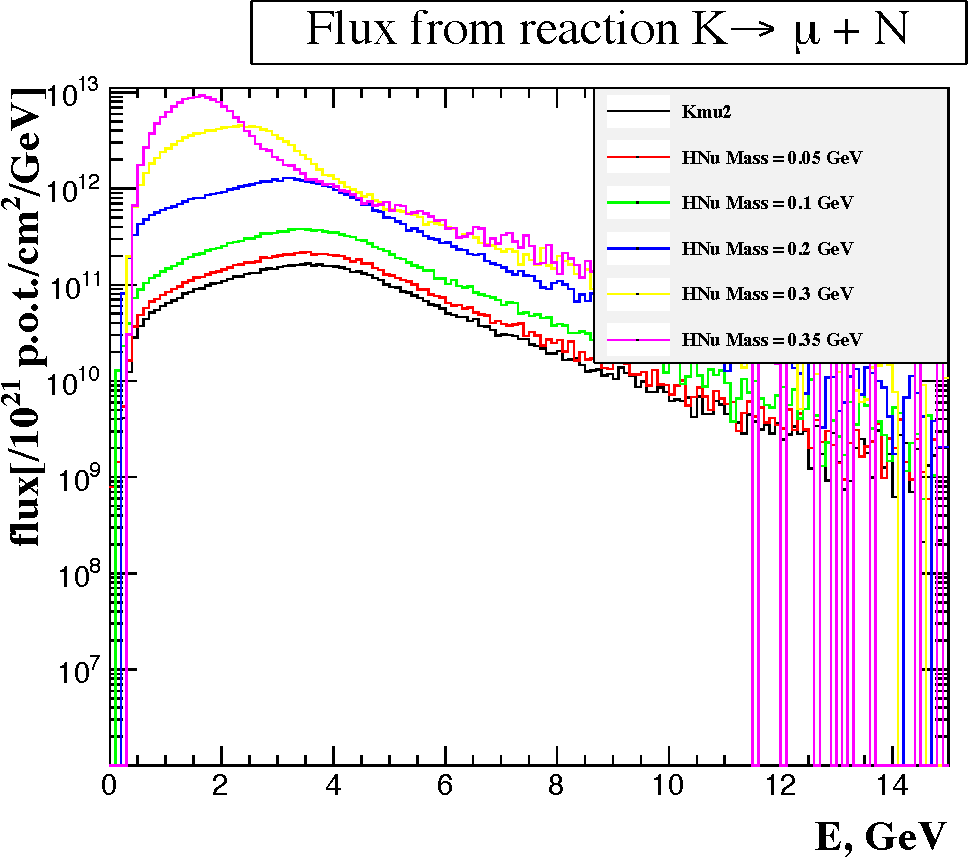
\includegraphics[width=\linewidth]{fluxKmu} \\ $K^+\rightarrow \mu^+N$}
    \end{minipage}
    \hfill
    \begin{minipage}{0.49\linewidth}
        \center{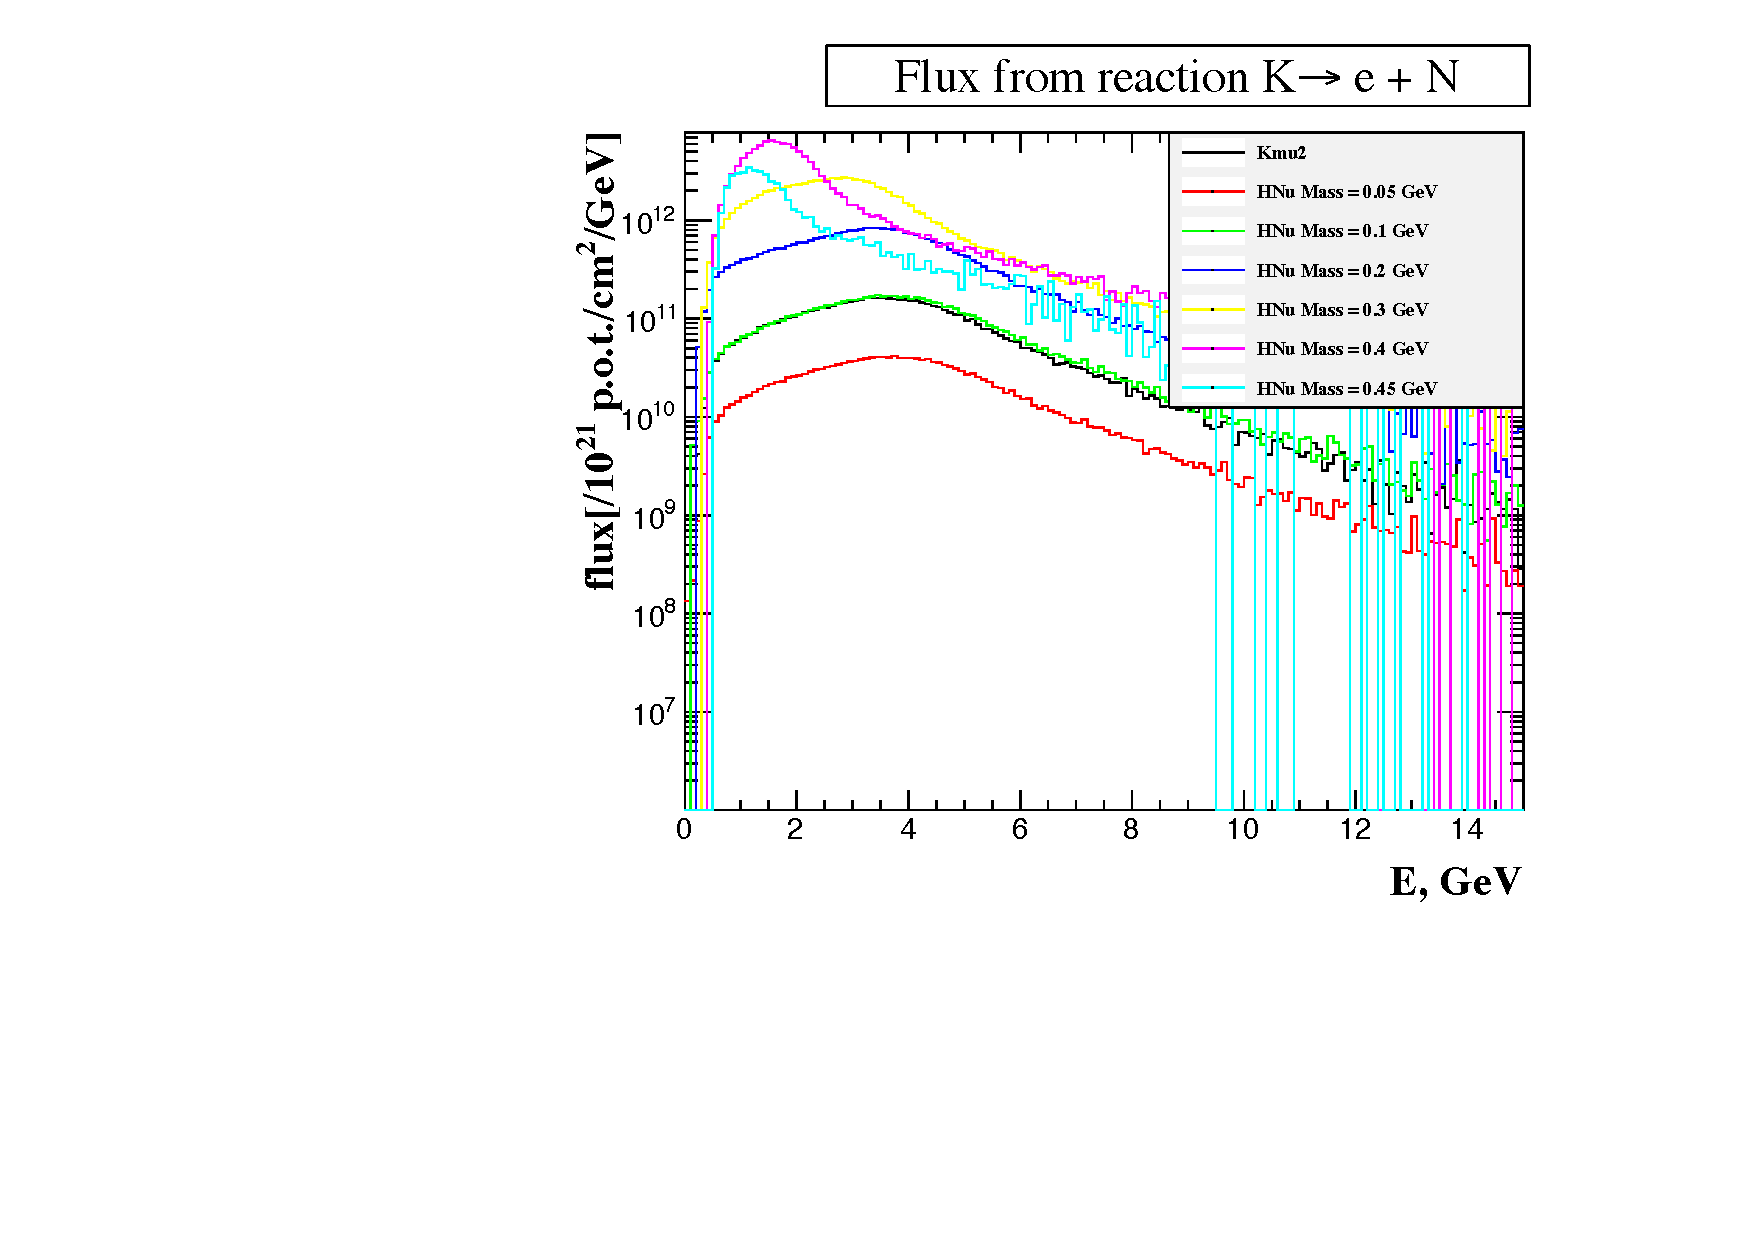
\includegraphics[width=\linewidth]{fluxKe} \\ $K^+\rightarrow e^+N$}
    \end{minipage}
    \caption{HNL energy spectra at the ND280 front plane for two modes: $K^+\rightarrow \mu^+N$ and $K^+\rightarrow e^+N$ for the different HNL masses.}
    \label{fig:HNL:fluxKpos}
\end{figure}

There are two effects, that cause the flux difference comparing to the active neutrino flux (\autoref{eq:HNL:weightDif}). The first one is ``massive'' kinematic of the parent meson decay. This correction is calculated according to~\autoref{eq:HNL:lorentz}. This impact is shown in~\autoref{fig:HNL:fluxMassKpos}. The branching ratio is assumed equal to 1.
\begin{figure}[!ht]
    \begin{minipage}{0.49\linewidth}
        \center{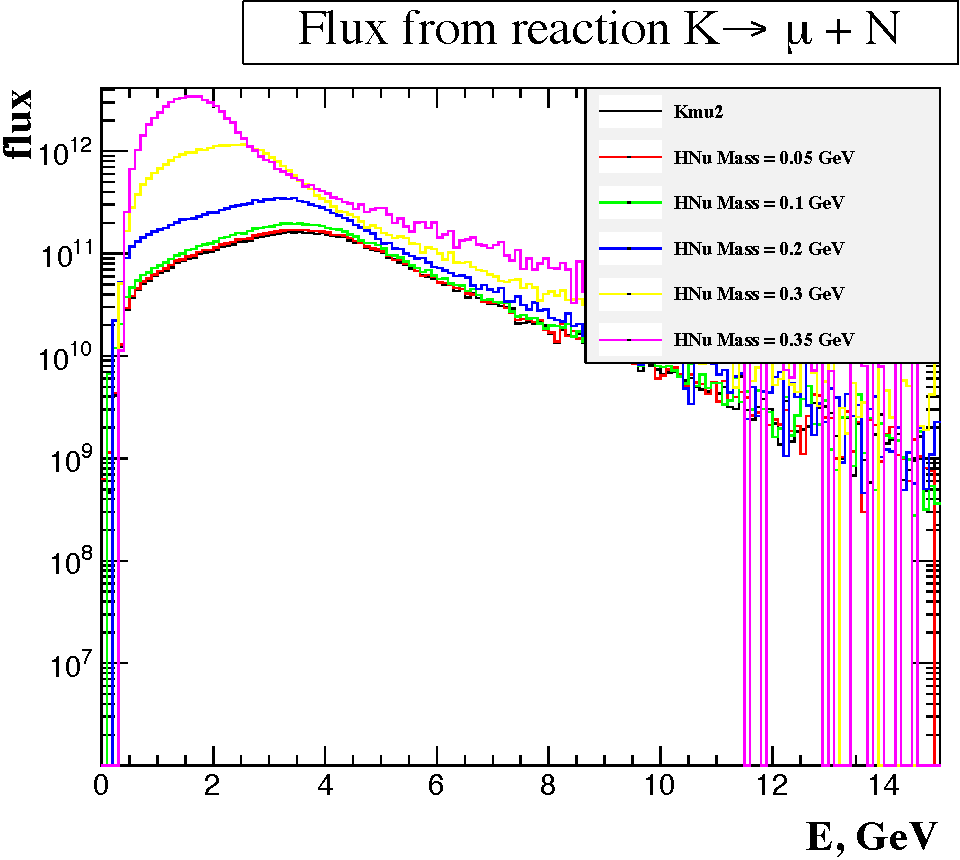
\includegraphics[width=\linewidth]{fluxMassKmu} \\ $K^+\rightarrow \mu^+N$}
    \end{minipage}
    \hfill
    \begin{minipage}{0.49\linewidth}
        \center{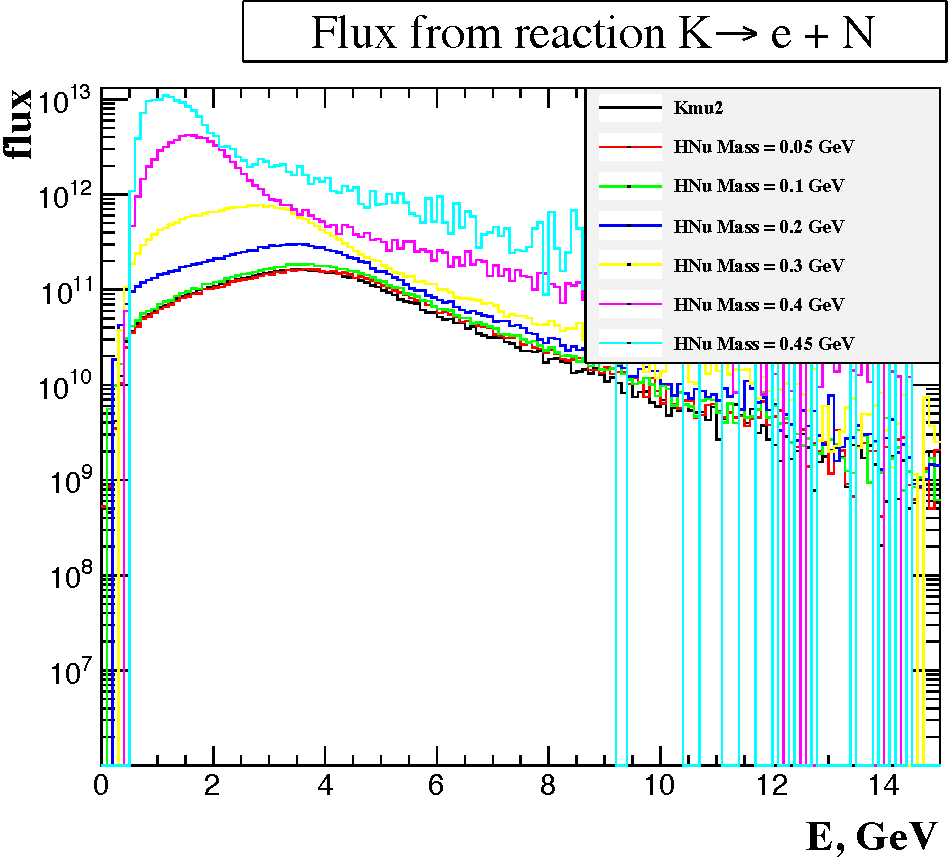
\includegraphics[width=\linewidth]{fluxMassKe} \\ $K^+\rightarrow e^+N$}
    \end{minipage}
    \caption{HNL spectra at the ND280 front plane for two modes and for the different HNL masses assuming the branching ratios equal to 1.}
    \label{fig:HNL:fluxMassKpos}
\end{figure}

The second effect is the modification of the branching ratio of the kaon decay. It is calculated according to~\autoref{eq:HNL:Kdecay}. The branching ratio dependence is shown in Fig.~\ref{fig:HNL:KdecayBR}.
\begin{figure}[!ht]
    \begin{minipage}[!ht]{0.49\linewidth}
        \center{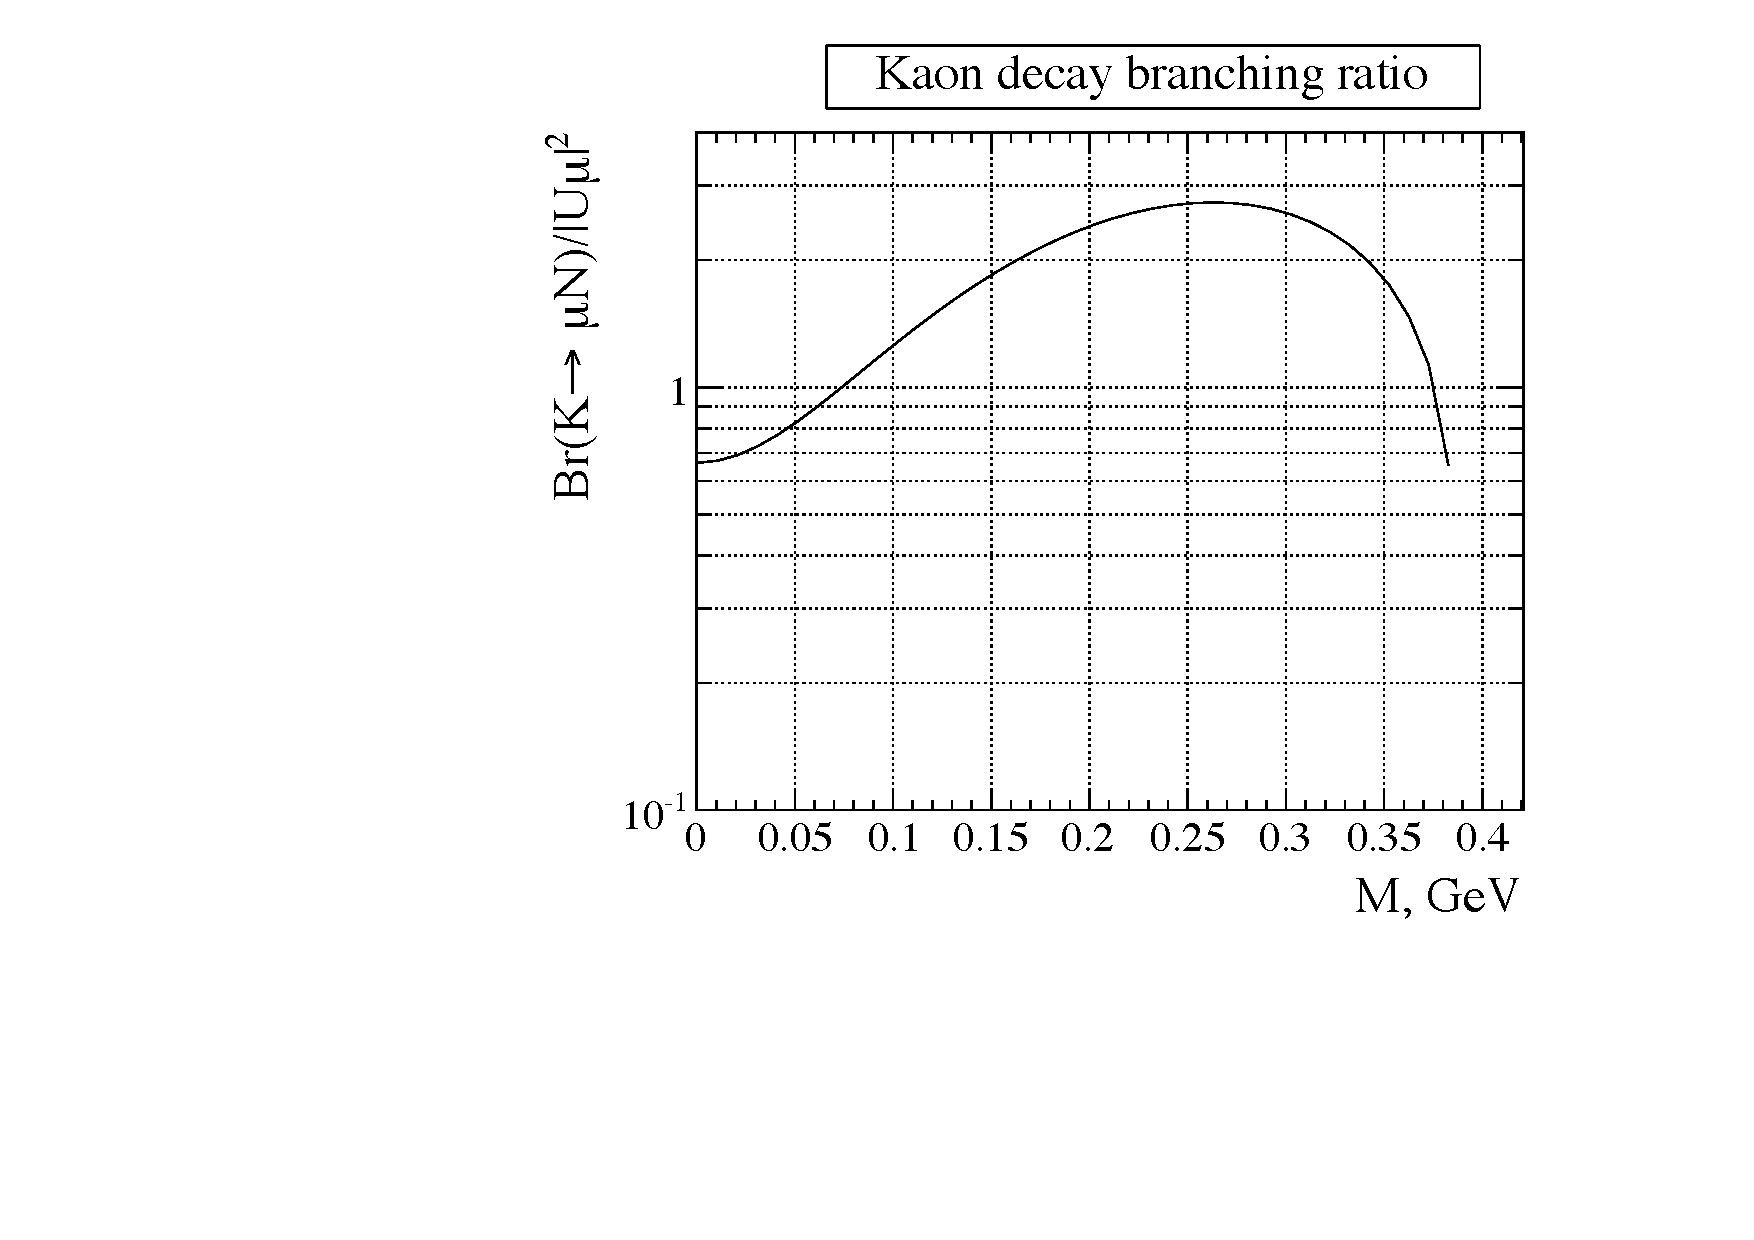
\includegraphics[width=\linewidth]{BrKMu} \\ a)}
    \end{minipage}
    \hfill
    \begin{minipage}[!ht]{0.49\linewidth}
        \center{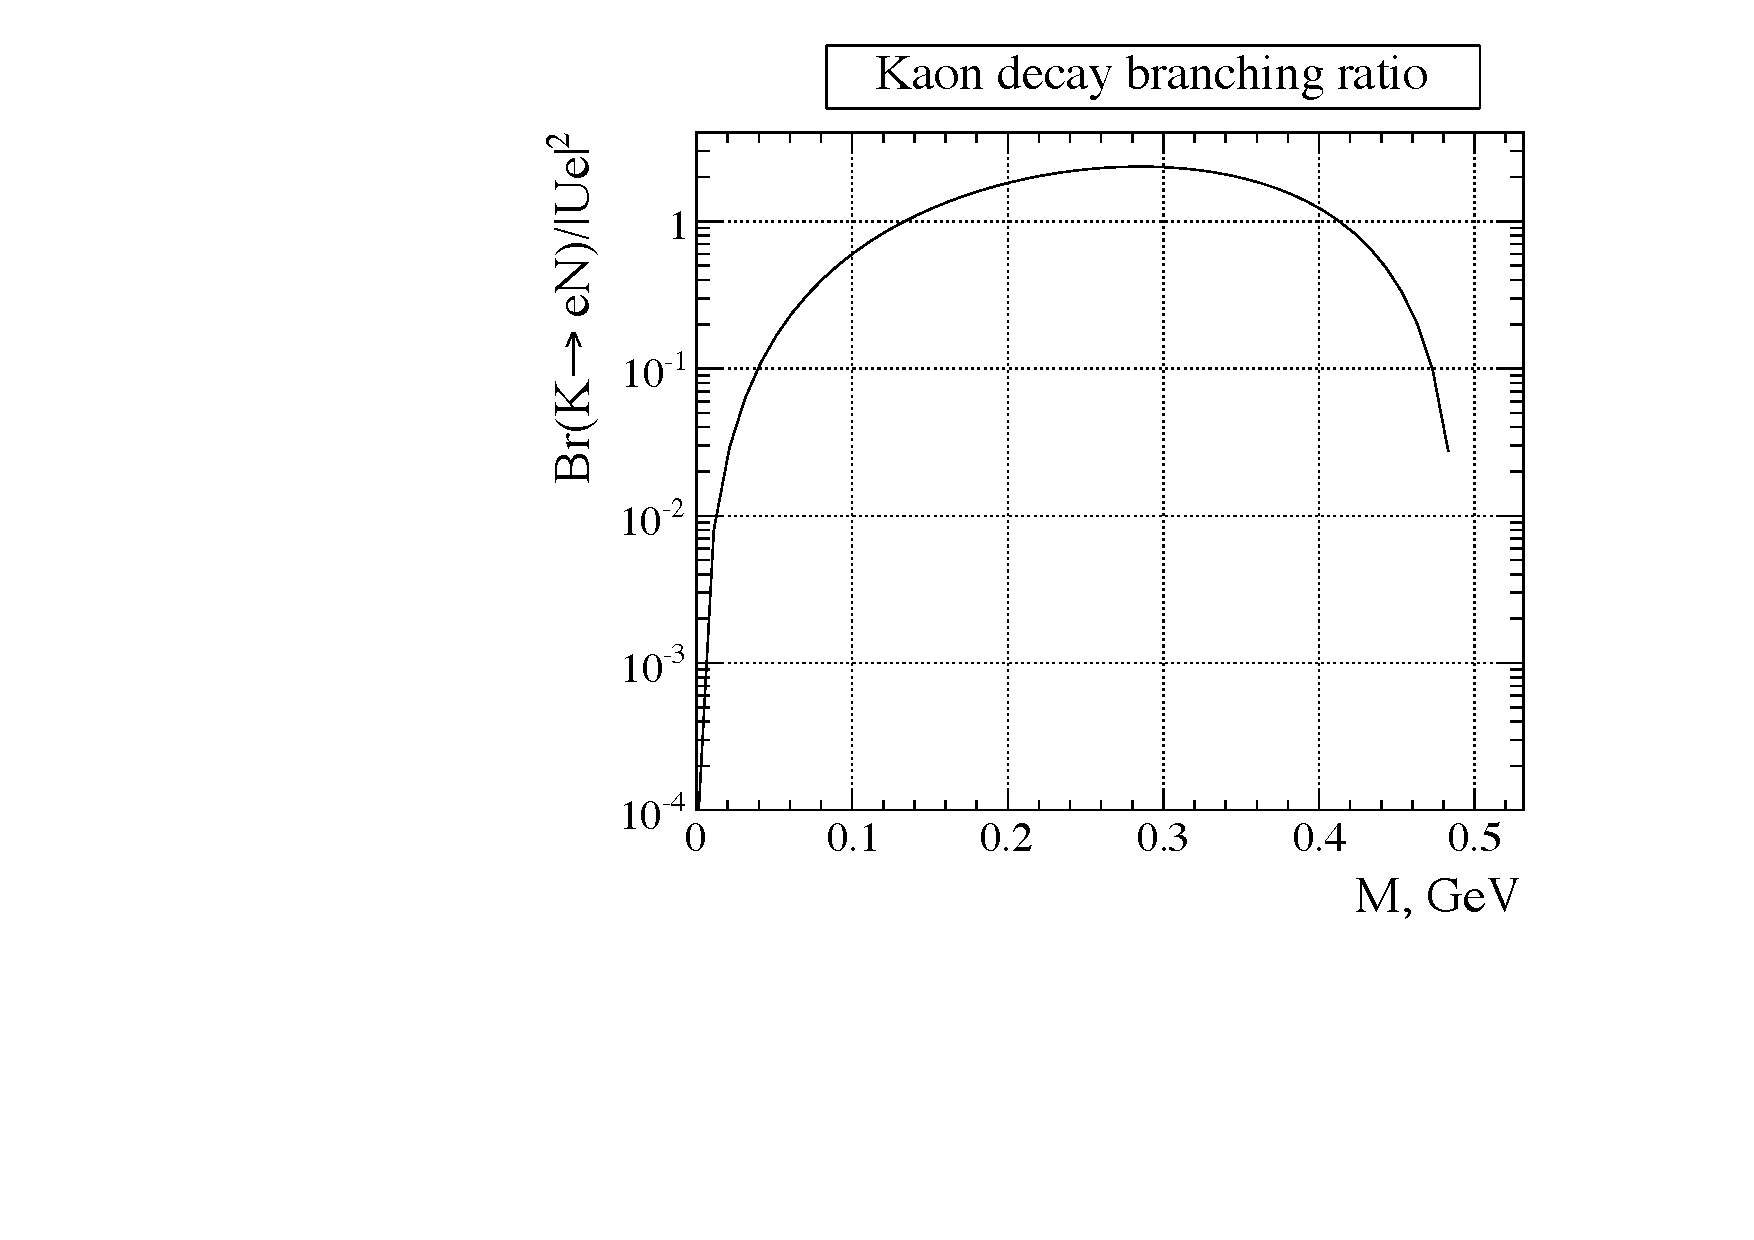
\includegraphics[width=\linewidth]{BrKEle} \\ b)}
    \end{minipage}
    \caption{Kaon decay branching ratio divided into the mixing element for two modes: (a) $K\to \mu N$ and (b) $K\to eN$.}
    \label{fig:HNL:KdecayBR}
\end{figure}

The difference of the time of flight for the active neutrino and HNL is described in the analysis~\autoref{sec:HNL:tof_corr}.

Since we study both $K^+$ and $K^-$ modes we compare HNL fluxes from both parent particles. The flux of HNL from $K^-$ decays is nearly three times lower than one from $K^+$ decays. It was expected since the cross section of $K^-$ production is approximately  tree times lower.

\section{HNL decays}

From the spectra of the heavy neutrinos, we can estimate the number of events from HNLs' decays and a sensitivity to mixing elements. As already described we just need the number of expected signal events. Number of decays is
\begin{equation}
    N_{decays}=\phi(HNL/10^{21}p.o.t./cm^2)\cdot S_{det} \cdot P_{decay}^{TPC}\cdot Br_{mode},
    \label{eq:HNL:Nevents}
\end{equation}
where
\begin{itemize}
    \item $\phi(HNL/10^{21}p.o.t./cm^2)$ --- the HNL flux per $10^{21}POT$ per $cm^2$;
    \item $S_{det}$ --- area of the ND280 front plane;
    \item $P_{decay}^{TPC}$ --- the probability of a HNL decay in one of 3 TPCs;
    \item $Br_{mode}$ --- branching of a current decay mode.
\end{itemize}
The decay probability between two points with coordinates $z_1$ and $z_2$, assuming large mean free path, is
\begin{equation}
    P_{decay}(z_2-z_1)=exp(-\frac{z_1}{c\beta\gamma\tau})-exp(-\frac{z_2}{c\beta\gamma\tau})\approx \frac{z_2-z_1}{c\beta\gamma\tau}
    \label{eq:HNL:Pdecay}
\end{equation}
where $\tau$ is HNL lifetime. Taking into account that
\begin{equation}
    Br_{mode}=\frac{\Gamma_{mode}}{\Gamma_{total}}=\Gamma_{mode}\cdot\tau,
\end{equation}
finally have
\begin{equation}
    N_{decays}=\phi(HNL/10^{21}p.o.t./cm^2)\cdot\frac{V_{FV}}{c\beta\gamma}\cdot\Gamma_{mode},
    \label{eq:HNL:EventsN}
\end{equation}
where $V_{FV}$ is a sum of the fiducial volumes of 3 TPC's. The decay width is calculated according to~\cite{Johnson1997, Gorbunov2007}. For 2-body decay we have
\begin{equation}
    \begin{split}
    \Gamma\left(N\to \pi^+\ell_\alpha^-\right)&=\frac{\left|U_\alpha\right|^2}{16\pi}G_F^2\left|V_{ud}\right|^2f_\pi^2M_{HNL}^3\left(\left(1-\frac{M_\ell^2}{M_{HNL}^2}\right)^2-\frac{M_{\pi}^2}{M_{HNL}^2}\left(1+\frac{M_\ell^2}{M_{HNL}^2}\right)\right)     \\
    &\times \sqrt{\left(1-\frac{\left(M_{\pi}-M_\ell\right)^2}{M_{HNL}^2}\right)\left(1-\frac{\left(M_{\pi}+M_\ell\right)^2}{M_{HNL}^2}\right)}
    \end{split}
\end{equation}
where  $\ell$ means lepton, $G_F$ --- Fermi constant, $f_\pi$ --- pion form-factor, $V$ --- CKM matrix element. The dependence of the decay width on the HNL mass is shown in~\autoref{fig:HNL:decBr}.

\begin{figure}[!ht]
    \begin{minipage}[!ht]{0.49\linewidth}
        \center{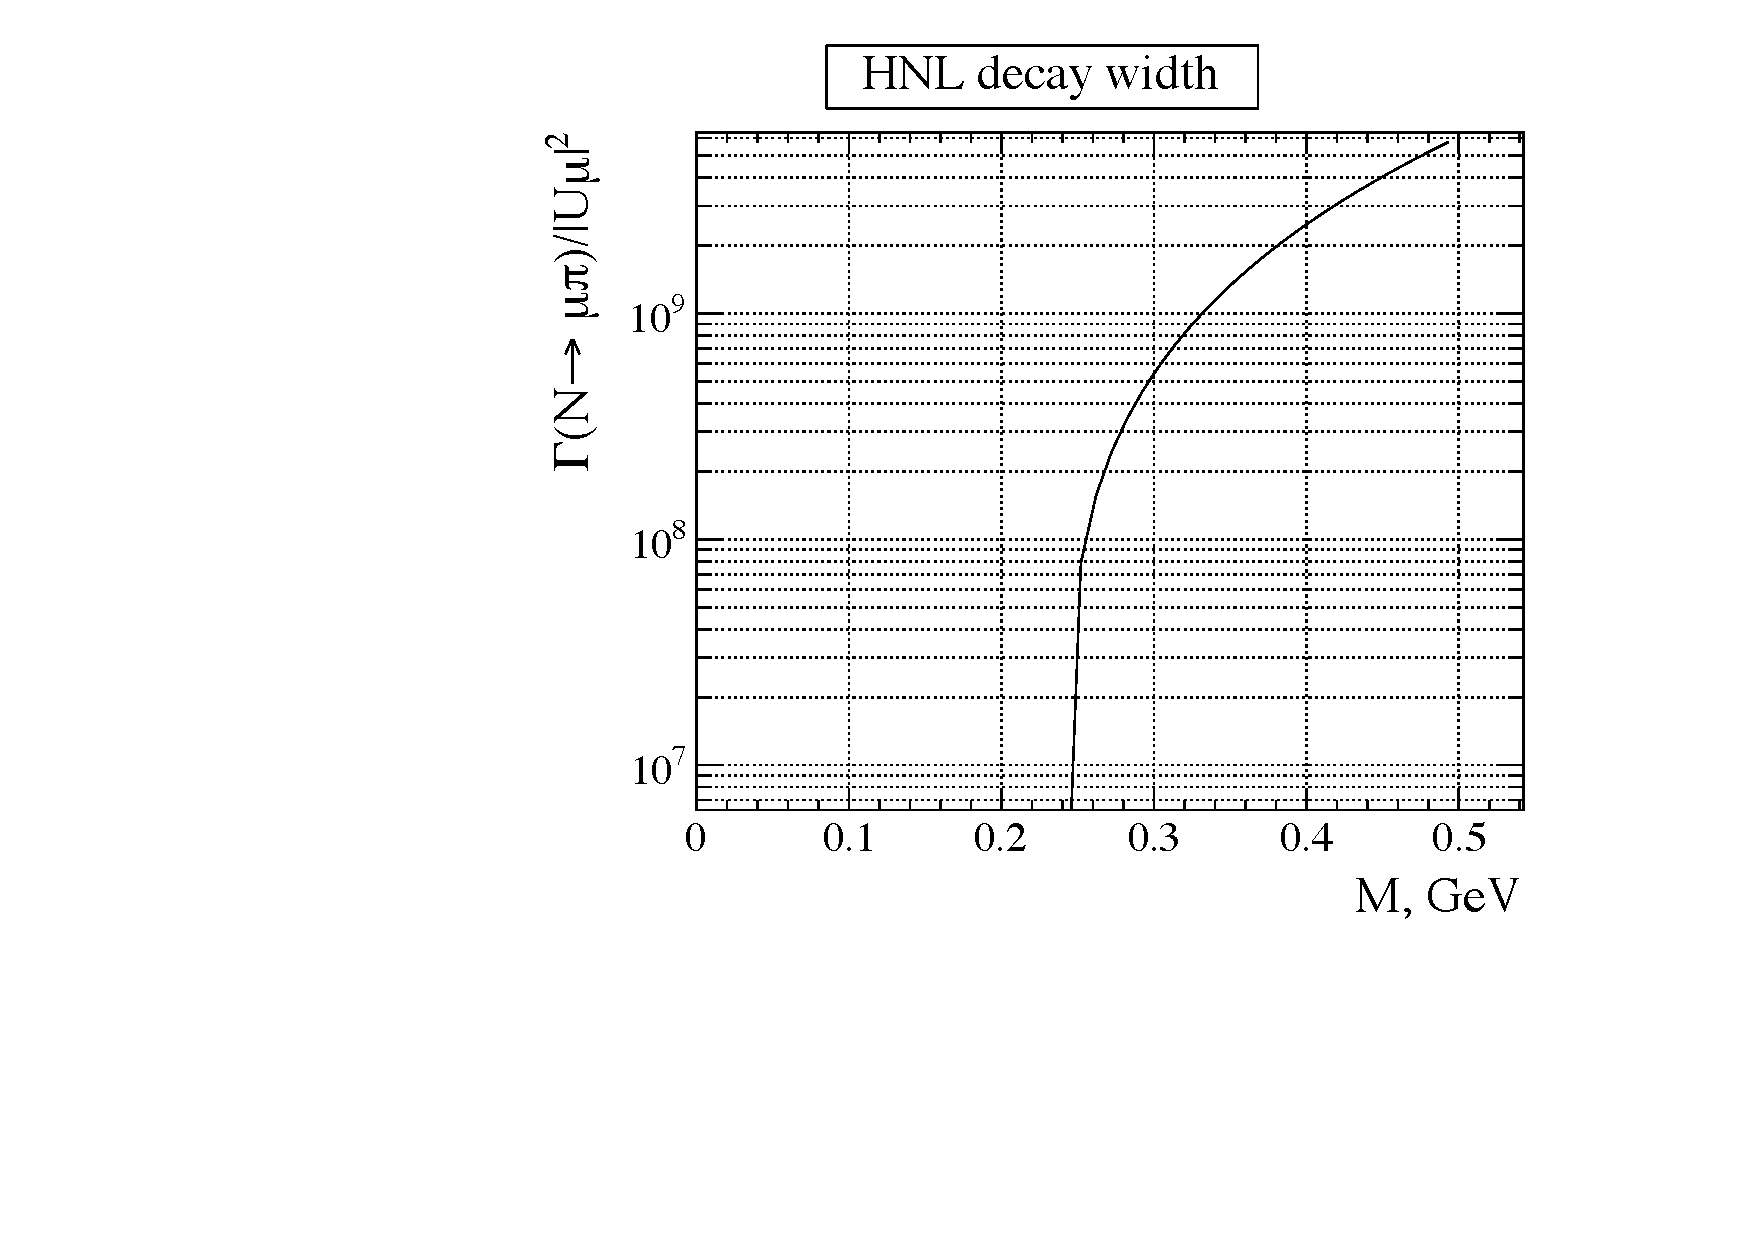
\includegraphics[width=\linewidth]{BrMu} \\ a)}
    \end{minipage}
    \hfill
    \begin{minipage}[!ht]{0.49\linewidth}
        \center{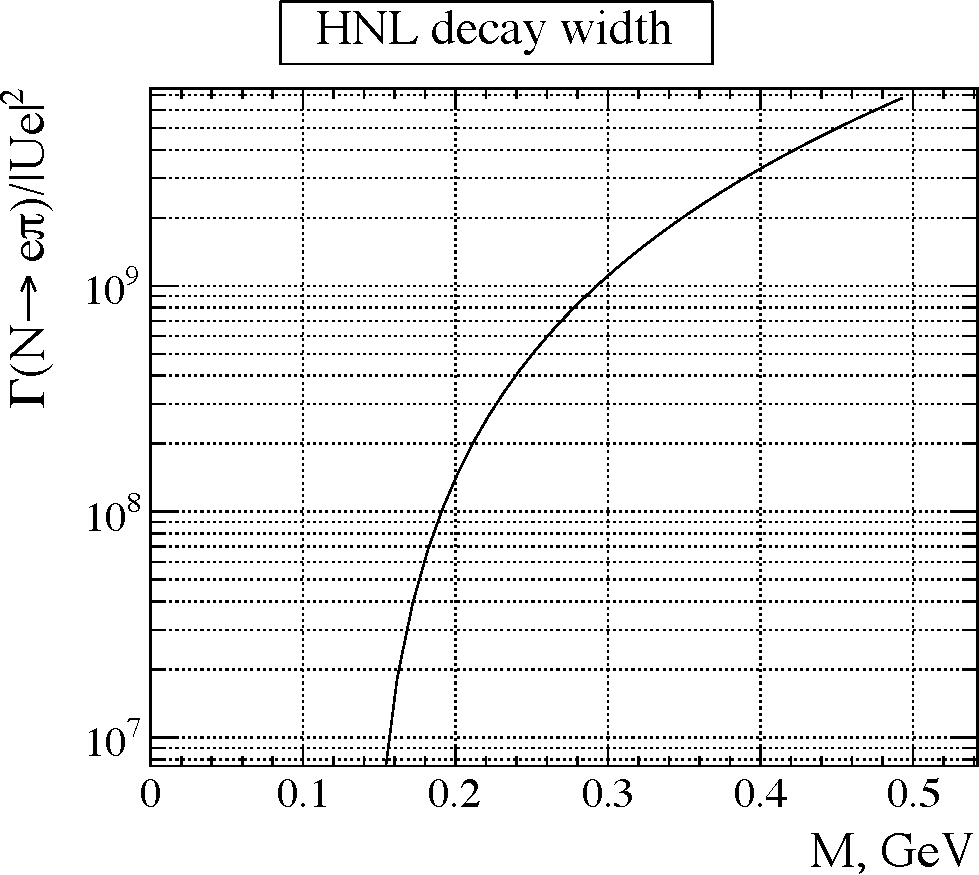
\includegraphics[width=\linewidth]{BrEle} \\ b)}
    \end{minipage}
    \caption{HNL decay width for two modes: (a) $N\to \mu\pi$ and (b) $N\to e\pi$ divided into the mixing element.}
    \label{fig:HNL:decBr}
\end{figure}

Based on the known number of expected decays we could evaluate the sensitivity of our experiment to the mixing elements. This estimation will be done for the optimistic scenario of the 100\% efficiency, no background and no systematic uncertainties. According to~\cite{Cousins1992} the 90\% C.L. could be set with 0 events observed and 2.3 events expected. As the HNL flux $\phi\propto\left|U\right|^2$ and the decay width $\Gamma_{mode}\propto\left|U\right|^2$:
\begin{equation}
    \left|U\right|^4_{limit} \times N_{decays} = 2.3
\end{equation}

Thus the limit on the squared mixing element will be put with:
\begin{equation}
    \left|U\right|^2_{limit}=\sqrt{\frac{2.3}{N_{decays}}},
\end{equation}
The sensitivity of our experiment for two body decays is shown in Fig.~\ref{fig:HNL:Ue2Umu2TwoBody}, ~\ref{fig:HNL:UeUmuTwoBody}, in green. It's compared with current limits from PS191~\cite{Bernardi1988} (in red) and Asaka et al prediction~\cite{Asaka2012} (in blue).
\begin{figure}[!ht]
    \begin{minipage}[!ht]{0.49\linewidth}
        \center{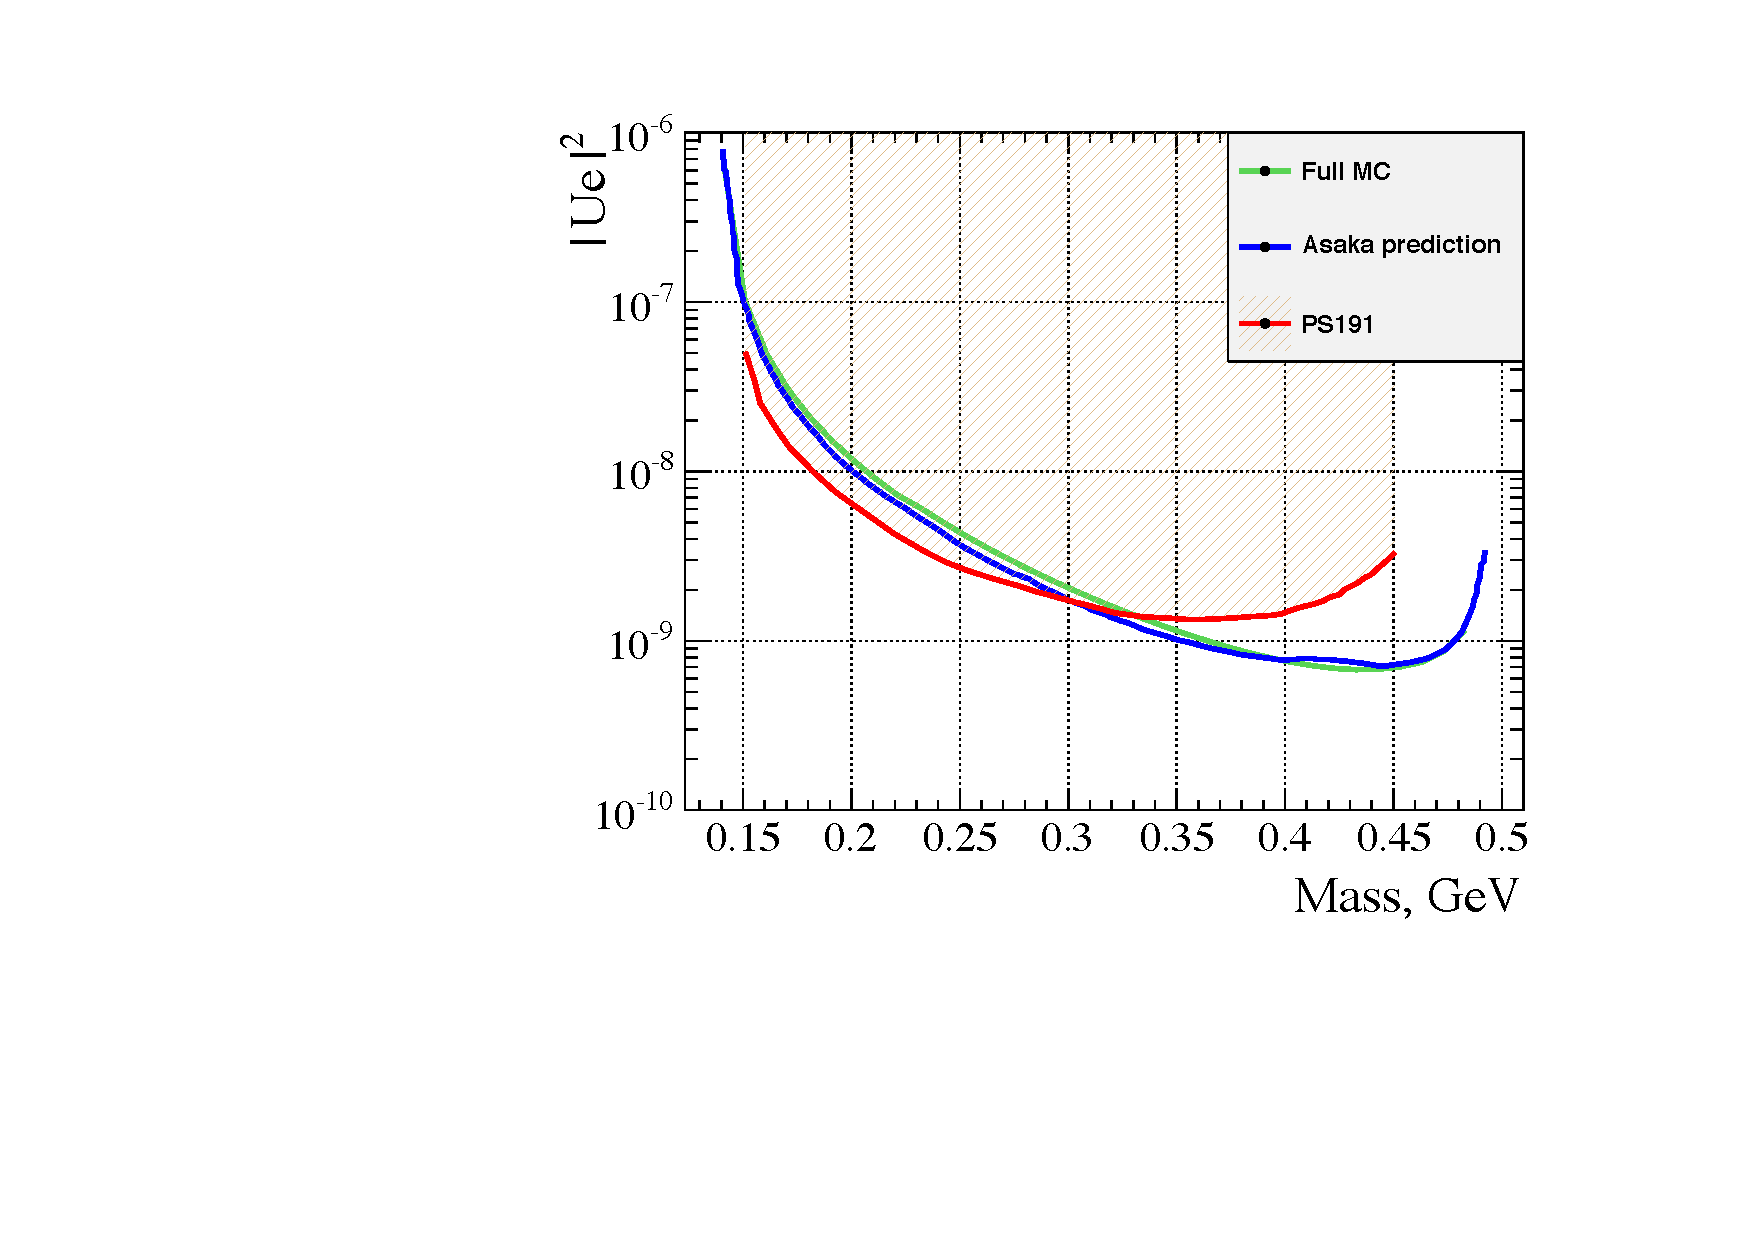
\includegraphics[width=\linewidth]{Ue2TwoBody} \\ a) $K\to eN\to e(e\pi)$}
    \end{minipage}
    \hfill
    \begin{minipage}[!ht]{0.49\linewidth}
        \center{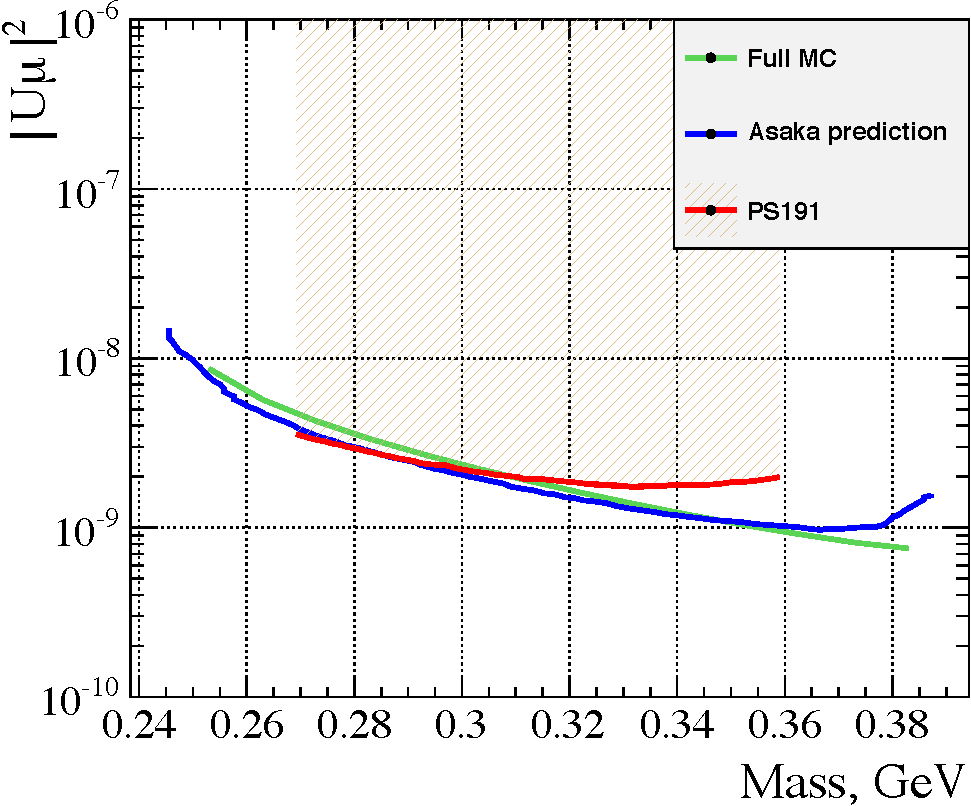
\includegraphics[width=\linewidth]{Umu2TwoBody} \\ b) $K\to\mu N\to \mu(\mu\pi)$}
    \end{minipage}
    \caption{Sensitivity of T2K to mixing element for two body decay modes for $10^{21}POT$. The detection efficiency of 100\% and no background are assumed.}
    \label{fig:HNL:Ue2Umu2TwoBody}
\end{figure}

\begin{figure}[!ht]
    \center{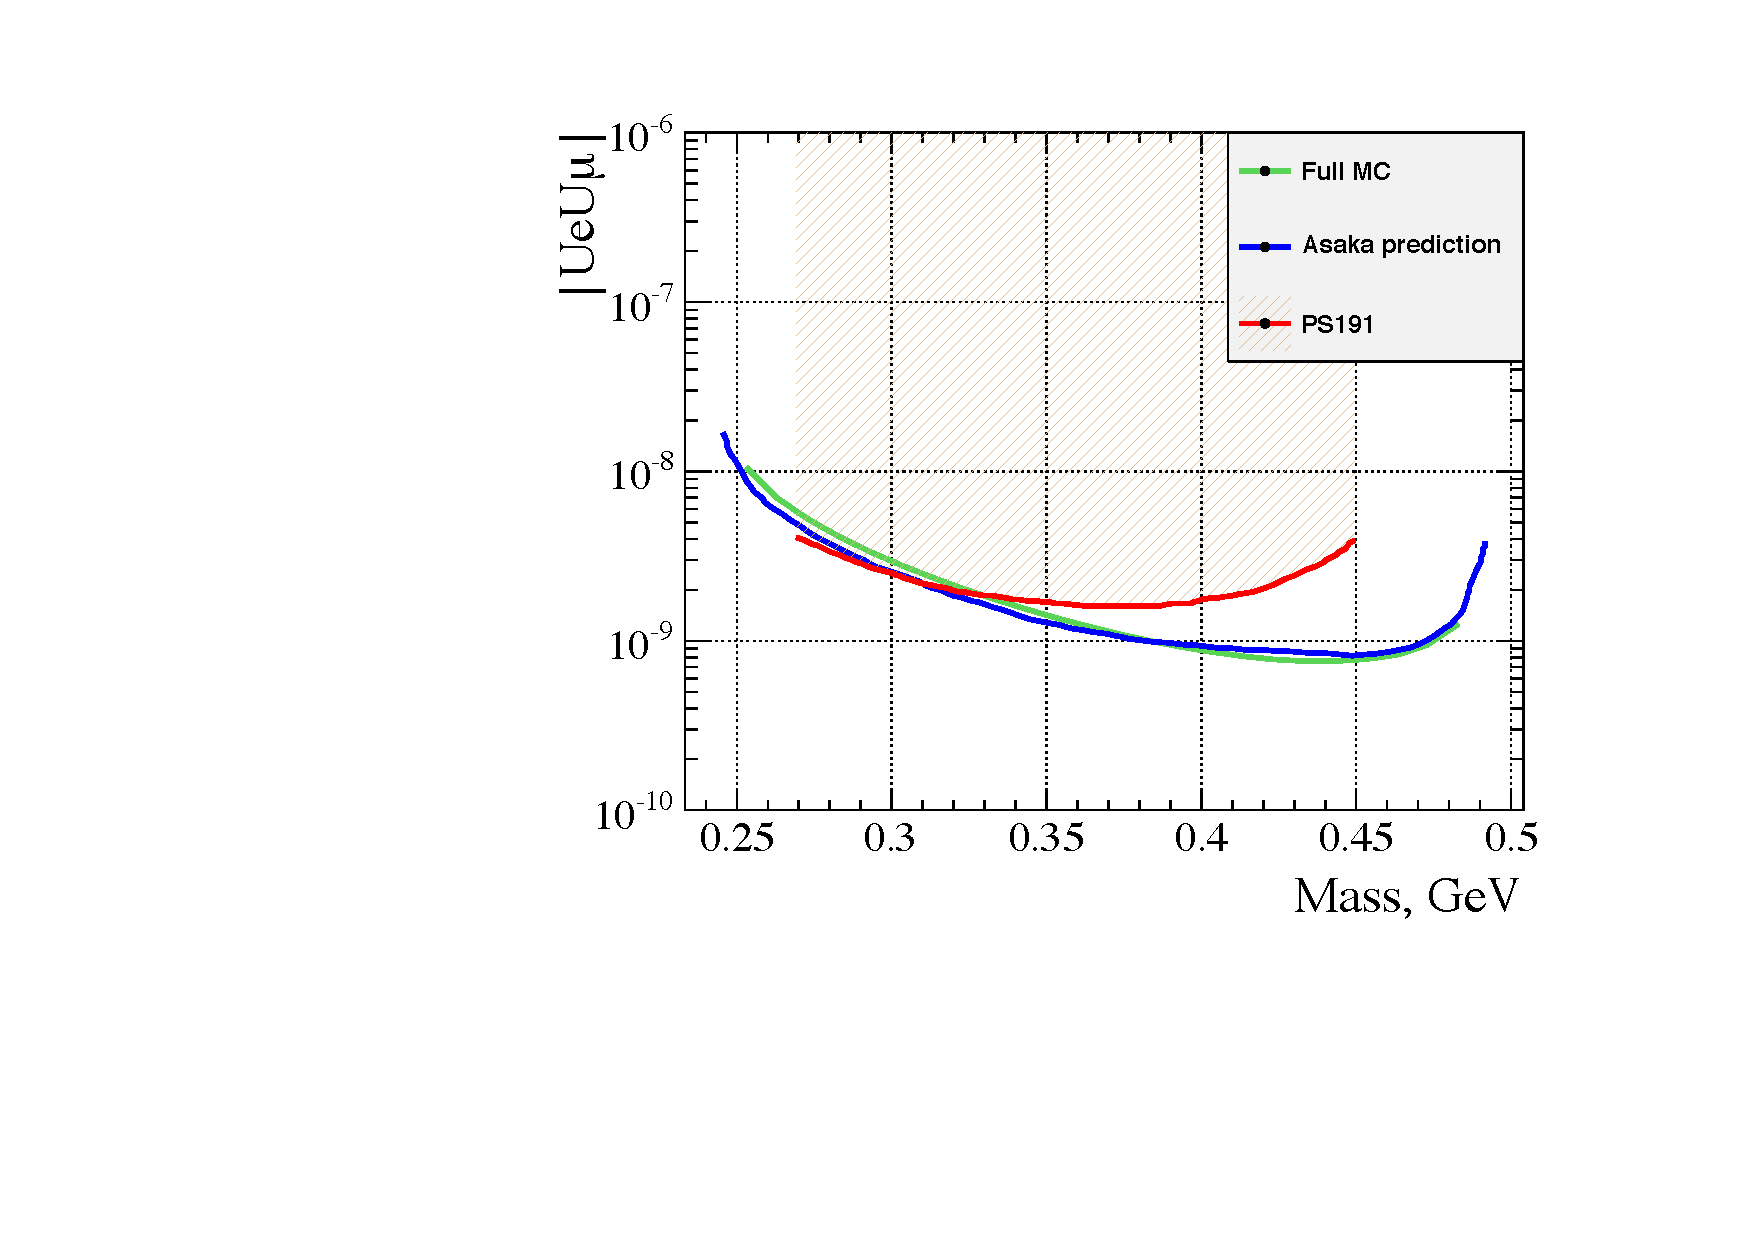
\includegraphics[width=0.49\linewidth]{UeUmuTwoBody}  \\ $K\to eN\to e(\mu\pi)$}
    \caption{Sensitivity of T2K to mixing element for two body decay modes for $10^{21}POT$. The detection efficiency of 100\% and no background are assumed.}
    \label{fig:HNL:UeUmuTwoBody}
\end{figure}

Three body decays of HNL were also studied. Possible improvement over the PS191 results is worse than for 2-body modes, the background for such events seems to be much larger due to the isotropic distribution of the charged daughter particles. In our study we will concentrate on 2-body decays and $N\to\mu\mu\nu$ mode. Three body sensitivity is shown in Fig.~\ref{fig:HNL:TreeBodyFirst} and Fig.~\ref{fig:HNL:ThreeBodySecond}.

\begin{figure}[!ht]
    \begin{minipage}[!ht]{0.49\linewidth}
        \center{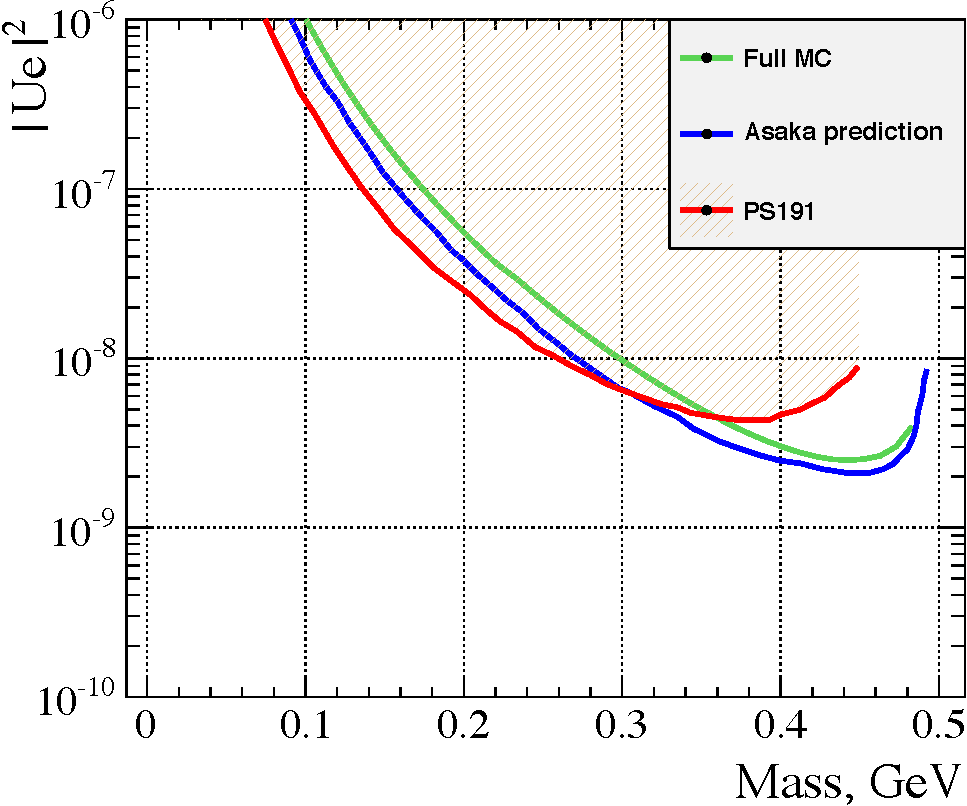
\includegraphics[width=\linewidth]{Ue2ThreeBody} \\ a) $K\to eN\to e(ee\nu_e)$}
    \end{minipage}
    \hfill
    \begin{minipage}[!ht]{0.49\linewidth}
        \center{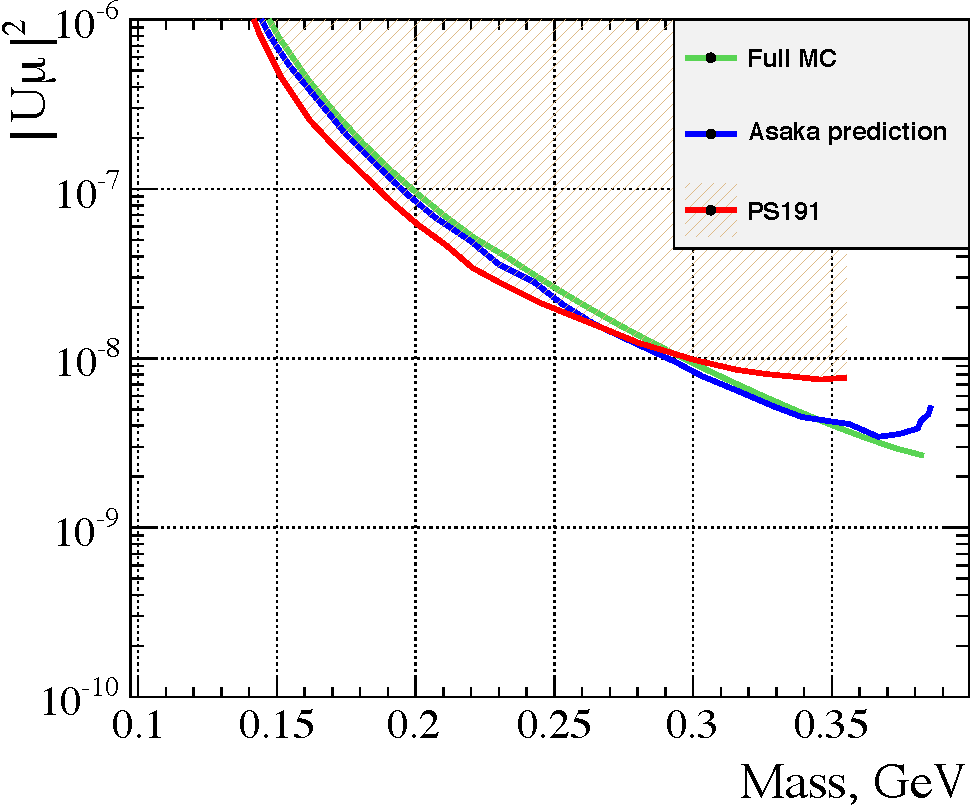
\includegraphics[width=\linewidth]{Umu2ThreeBody} \\ b) $K\to \mu N\to \mu(\mu e\nu_e)$}
    \end{minipage}
    \caption{Sensitivity of T2K to mixing element for three body decay modes for $10^{21}POT$. The detection efficiency of 100\% and no background are assumed.}
    \label{fig:HNL:TreeBodyFirst}
\end{figure}

\begin{figure}[!ht]
    \begin{minipage}[!ht]{0.49\linewidth}
        \center{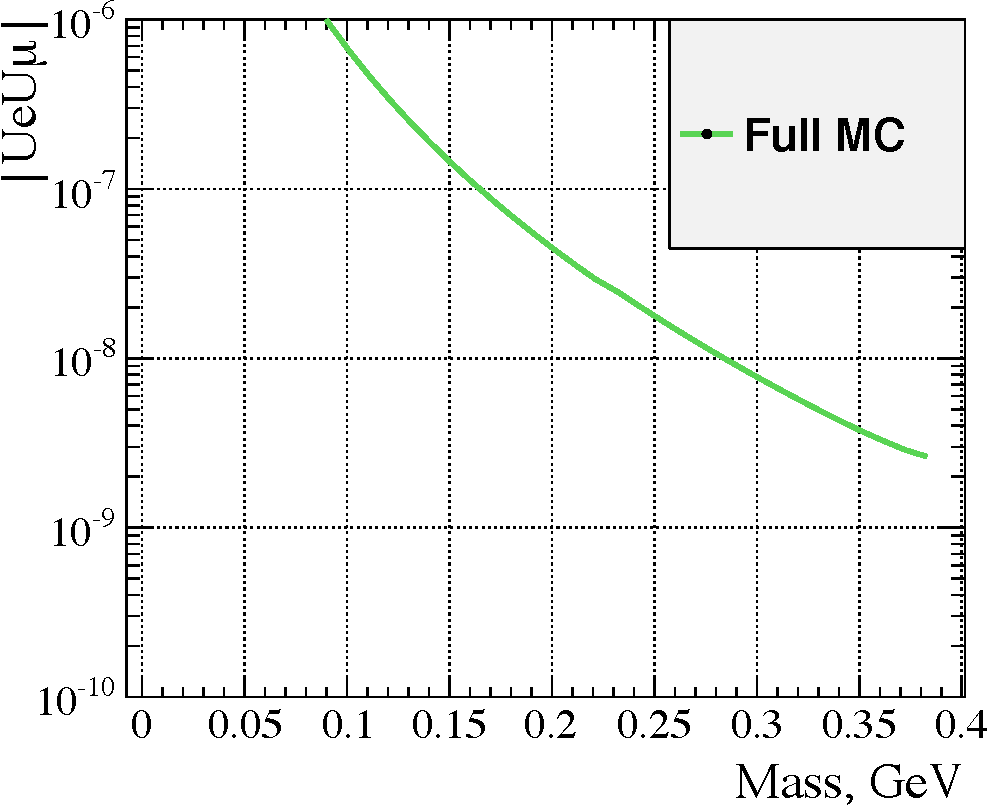
\includegraphics[width=\linewidth]{UmuUeThreeBody}  \\ a) $K\to\mu N\to \mu(ee\nu_e)$}
    \end{minipage}
    \hfill
    \begin{minipage}[!ht]{0.49\linewidth}
        \center{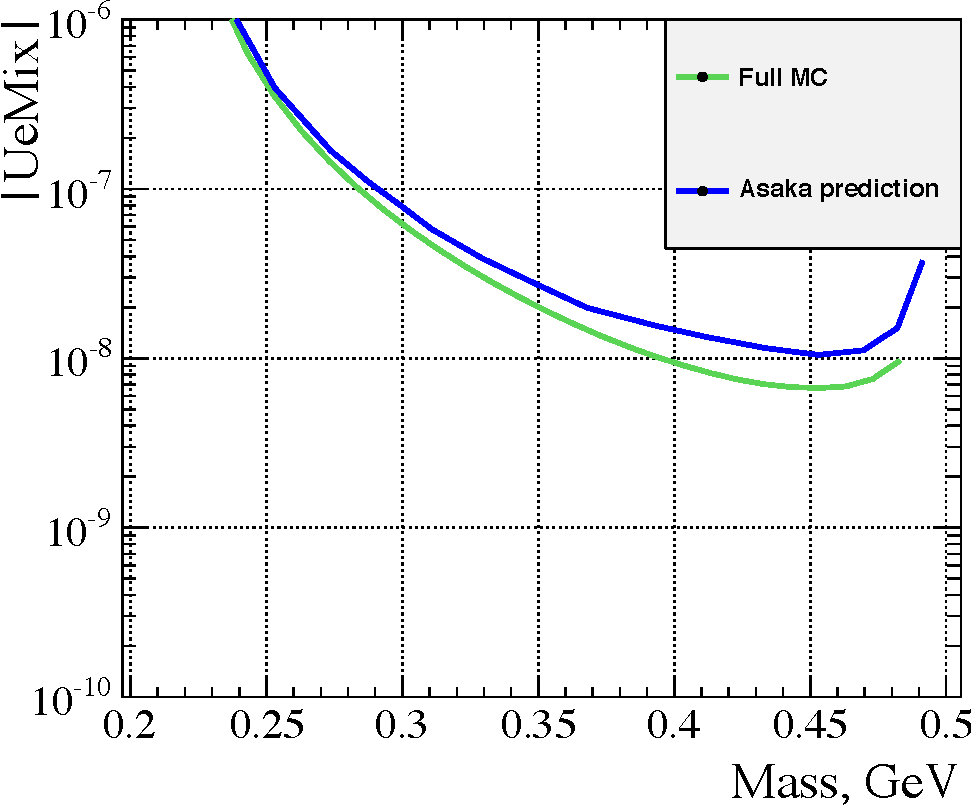
\includegraphics[width=\linewidth]{UeMixThreeBody} \\ b) $K\to eN\to e(\mu\mu\nu_{\mu,\tau})$}
    \end{minipage}
    \caption{Sensitivity of T2K to mixing elements in tree body decay modes: (a) for $\left|UeU\mu\right|$ and (b) for $\left|U_{e}\right|\sqrt{\left|U_{e}\right|^2+\left|U_{\tau}\right|^2}$. The detection efficiency of 100\% and no background are assumed.}
    \label{fig:HNL:ThreeBodySecond}
\end{figure}

An important 3-body mode is $K^+\rightarrow e(\mu^-\mu^+\nu_{e,\mu,\tau})$ because $\ell\bar{\ell}$ pairs can be produced together with any kind of the active neutrino due to  the NC process ~\cite{Johnson1997}. The mixing element for this process looks like $\left|U_{e}\right|\sqrt{\left|U_{e}\right|^2+\left|U_{\mu}\right|^2+\left|U_{\tau}\right|^2}$. Assuming $\left|U_e\right|^2 \gg\left|U_{\mu}\right|^2$, we can get some constraints on $\left|U_{e}\right|\sqrt{\left|U_{e}\right|^2+\left|U_{\tau}\right|^2}$ that wasn't obtained before in PS191 and limits on $\left|U_{\tau}\right|$ are also rather poor. Results for this decay mode are shown in Fig. ~\ref{fig:HNL:ThreeBodySecond} b.

As one can see, all our results are close to the estimation made by Asaka et al.

\subsection{HNL daughter particles}
Now we have all the information about the HNLs that enter ND280. Thus we could generate the secondary particles that will be born in the heavy neutrino decay. The decay itself is simulated in the HNL rest frame. Then the boost is applied towards the heavy neutrino initial direction. The decay points are randomly generated along the  HNL tracks inside the TPC volume. So the decay positions are expected to be uniformly distributed in this volume. Cross-check (Fig.~\ref{fig:HNL:decayPos}) shows some deviations at the upper and bottom edges for the large HNL mass but it was also expected due to the off-axis flux.

The simulation of the 2-body decay is straight forward. The direction of the first particle is thrown isotropically. Then base on both momentum and energy conservation laws all the decay is parametrized in the HNL rest frame. We will obtain the final kinematics of the daughters with the boost along the heavy neutrino momentum. For the each event the following weight is assigned:
\begin{equation}
    weight_{2-body}=weight_{K\rightarrow \ell N}\cdot\frac{L}{\beta\gamma c}\cdot\Gamma_{2-body},
\end{equation}

The 3-body decay case is a bit more complicated. For this case we can't just throw all the directions as we have one degree of freedom in the decay. To deal with it we used the normalization with the maximum width of the decay. For each event the following weight is assigned:

\begin{equation}
    weight_{3-body}=weight_{K\rightarrow \ell N}\cdot\frac{L}{\beta\gamma c}\cdot\cfrac{\cfrac{d\Gamma(p_1,p_2)}{dp_1dp_2}}{max\left(\cfrac{d\Gamma(p_1,p_2)}{dp_1dp_2}\right)}\cdot P,
\end{equation}

where $L$ is total length of HNL path in three TPCs. We normalize the weight of each particular decay with respect to the maximum possible value. This will make the absolute number of the events smaller, but as we use the signal sample only for the efficiency evoluation the effect will be compensated. That's important as the selection probability could depend on the kinematics and we need to assign proper weight to each generated event for proper efficiency treatment.

\begin{figure}[!ht]
    \center{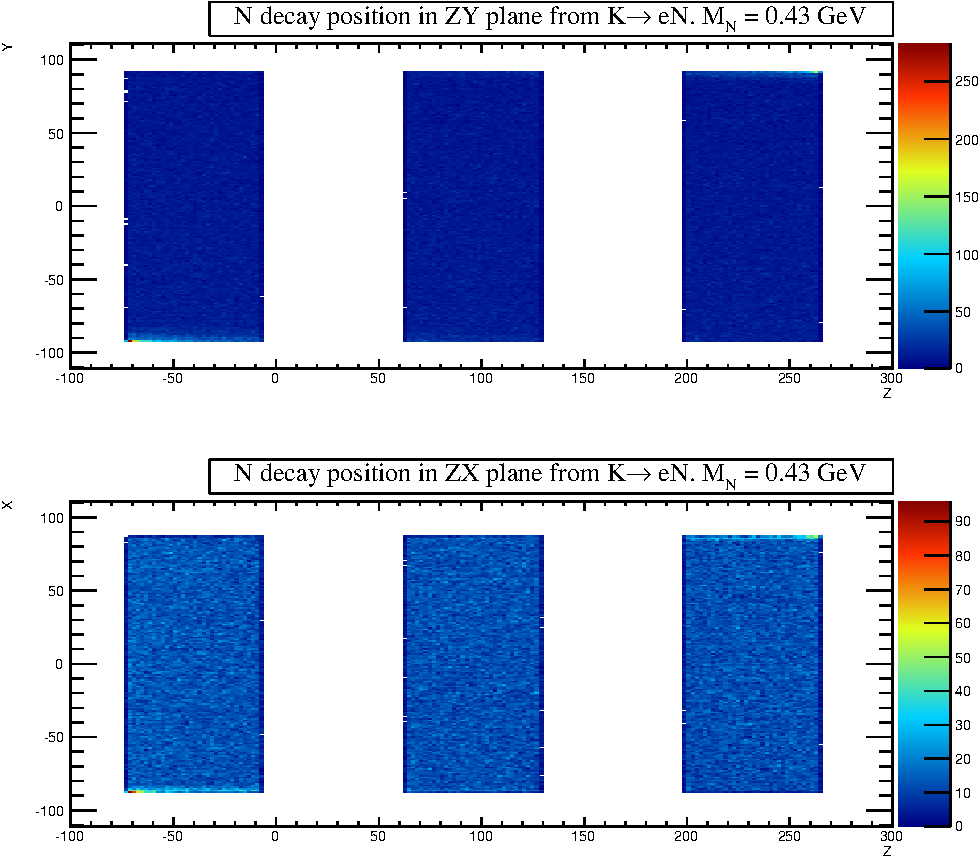
\includegraphics[width=0.7\linewidth]{DecayPos}}
    \caption{Distribution of HNL decay positions over 3 TPCs. The decay position is in the detector coordinate system in mm.}
    \label{fig:HNL:decayPos}
\end{figure}

\todo{HNL polarization description}

After simulation of the HNL decays we have all information about kinematics of their daughter particles, i.e. momentum, direction, opening angles. This characteristics are presented in~\autoref{fig:HNL:secondaryE}~and~\autoref{fig:HNL:secondaryCos}. It's important to note that most of the particles have momentum below 2 GeV. Our TPCs was designed to reconstruct events in this energy region.
\begin{figure}[!ht]
\begin{center}
    \center{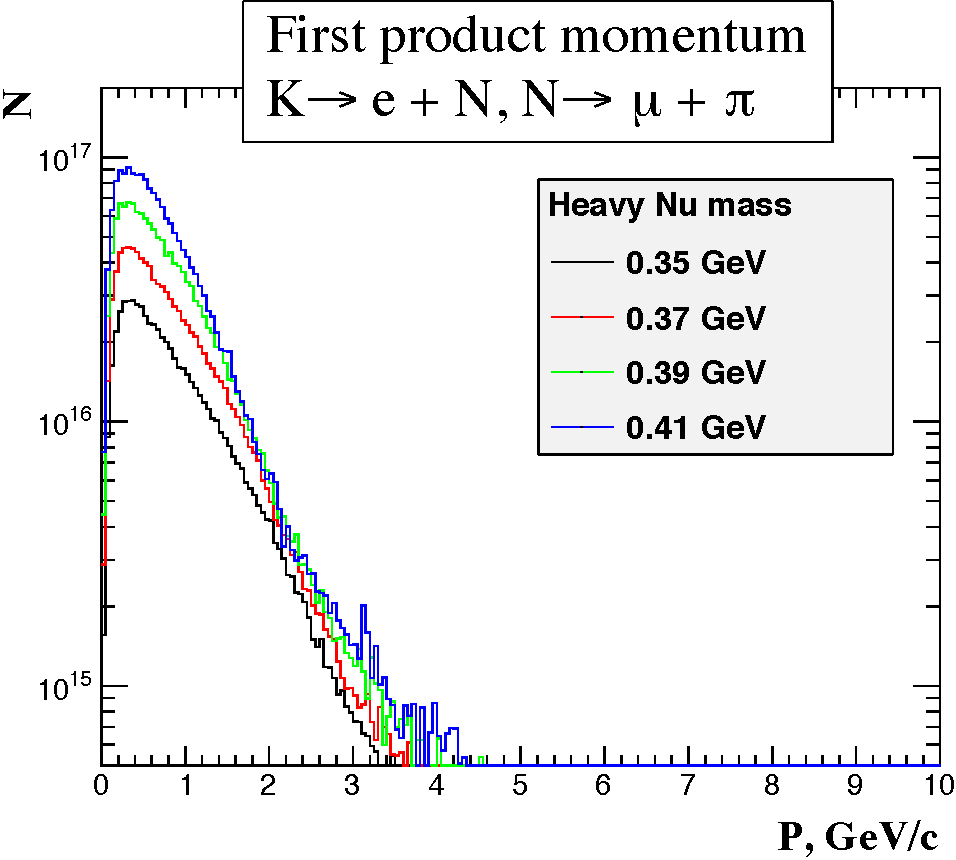
\includegraphics[width=0.8\linewidth]{SecMom}}
    \caption{Energy spectra of HNL daughter particles.}
    \label{fig:HNL:secondaryE}
\end{center}
\end{figure}
\begin{figure}[!ht]
\begin{center}
    \center{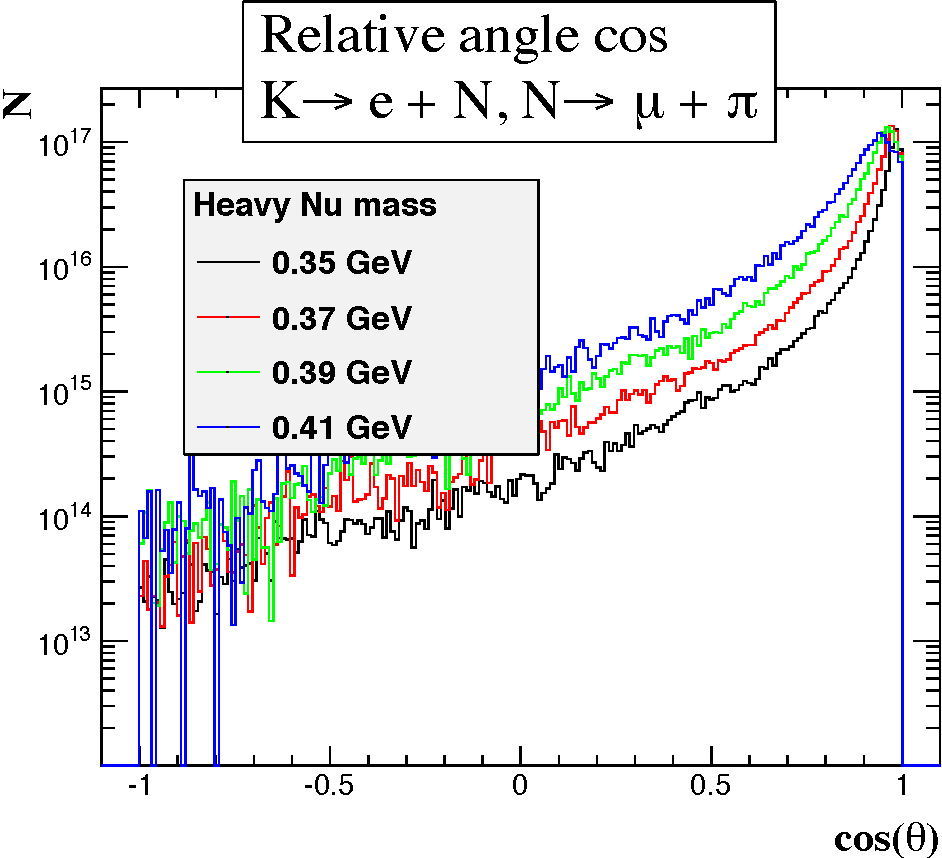
\includegraphics[width=0.8\linewidth]{SecRel}}
    \caption{Opening angle spectra of HNL daughter particles.}
    \label{fig:HNL:secondaryCos}
\end{center}
\end{figure}
The heavy neutrino daughter particles are propagated through the detector with the help of the Geant4 package~\cite{Agostinelli2003}. All the secondary interactions, decays, etc. are considered.
The example of a ``good'' MC event with the HNL decay in the first TPC and further evolution of a daughter muon and a pion is shown in Fig.\ref{fig:HNL:event}. The detector response is fully simulated from the initial ionization until the readout signal from the electronics. Thus we could develop the event selection and estimate its efficiency with the MC generated signal sample.
\begin{figure}[!ht]
   \center{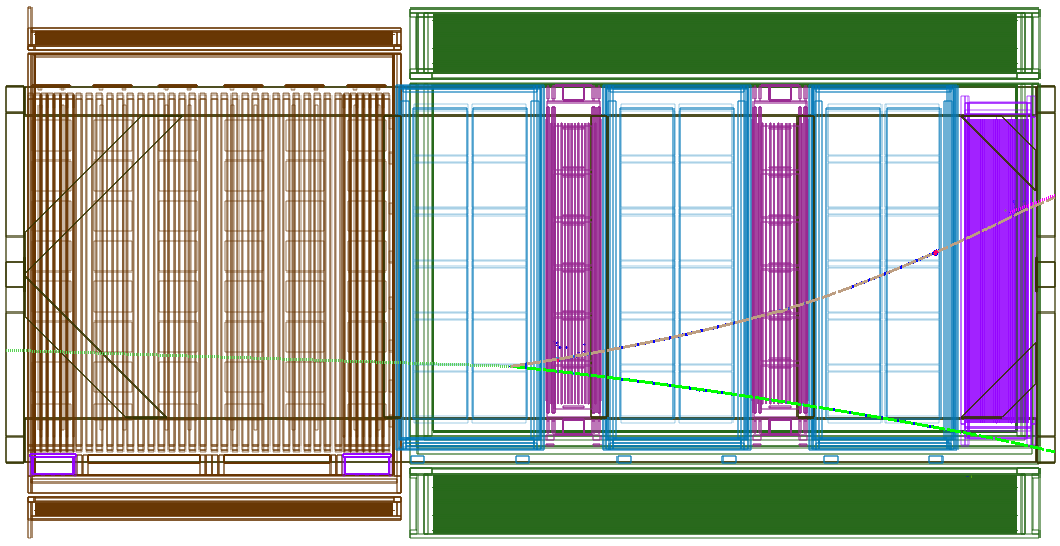
\includegraphics[width=0.8\linewidth]{goodeventMC}}
    \caption{Example of simulated event from HNL decay in the first TPC. Dashed green line corresponds to HNL track, green line to the muon track, brown line to the pion track.}
    \label{fig:HNL:event}
\end{figure}

\chapter{HNL analysis}
\label{ch:HNL:ana}
The search for heavy neutrino consists of several parts. At the first step we apply the time correction to the signal sample. The correction is related to the time delay of the HNL with respect to the neutrino bunch. The details are presented in the~\autoref{sec:HNL:tof_corr}. Then the cut sequence was developed in order to select signal and suppress the background events. The details about the selection are described in the~\autoref{sec:HNL:sel}. Controlling the uncertainties is an important part of any analysis. In our case the uncertainties will come from the detector response simulation and flux prediction (\autoref{sec:HNL:sys}). Finally we choose the appropriate statistical method for the results treatment (\autoref{sec:HNL:stat}).

\section{Time of flight correction}
\label{sec:HNL:tof_corr}
Heavy neutrino time of flight is different from the active neutrino. The difference is calculated according to Eq.~\ref{eq:HNL:ToF}.
\begin{equation}
  \delta T=\frac{d}{\beta c}-\frac{d}{c}=\frac{d}{c}\left(\frac{1}{\beta}-1\right),
  \label{eq:HNL:ToF}
\end{equation}
where $d$ is a distance between the HNL production and decay points, $\beta=\frac{v}{c}$ is a kinematic parameter of the HNL. The ToF modeling is not performed during the HNL simulation. So we apply the correction $T'=T+\delta T$ in the analysis, shifting all timestamps in the event by the $\delta T$. In the T2K the  neutrino beam repeats the proton beam spill structure with 8 bunches. The bunches are Gaussian with $\sigma\approx19ns$ (\autoref{ch:T2K:nu_beam}). Due to the ToF correction the HNL bunch will change its shape. The new bunch structure is shown in~\autoref{fig:HNL:bunch}.
\begin{figure}[!ht]
  \begin{center}
  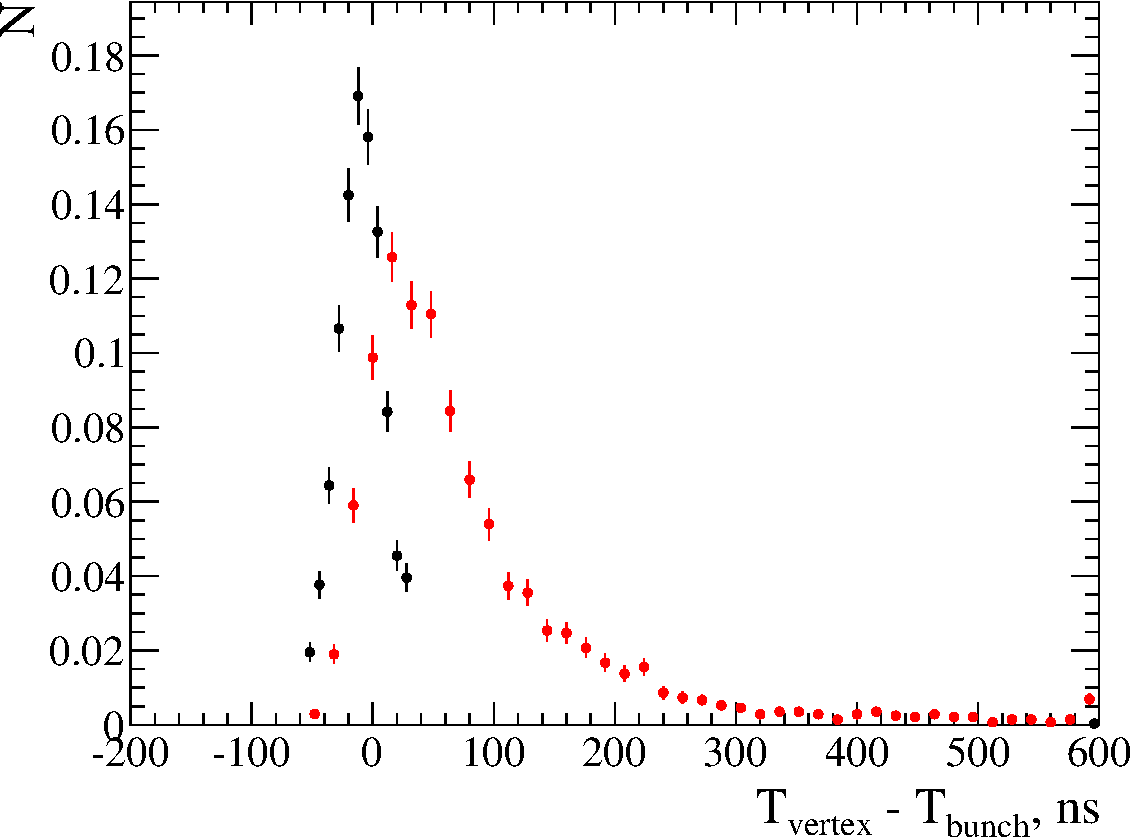
\includegraphics[width=0.7\linewidth]{Bunch}
  \caption{The active neutrino bunch (in black) and the HNL bunch (in red) for $M_{HNL}=480MeV$.}
  \label{fig:HNL:bunch}
  \end{center}
\end{figure}

For active neutrino analysis the standard time gate is $\left|T_{event}-T_{bunch}\right|<60ns$. By the $T_{bunch}$ the mean value of the Gaussian distribution is considered. In our analysis we should widen the time window in order to increase the efficiency of the selection. Since the shape of the HNL bunch is asymmetric, we applied different cuts value for upper and lower boundaries of the time window. For the bounds we are limited by the electronics time gate. As the experimental setup was originally designed to deal with neutrino bunches the data recording time was limited. We widen the cut values as much as the data acquisition allow us to do it and put the limits to $-100ns<T_{vertex}-T_{bunch}<300ns$.

We do not apply any additional time of flight cut to separate interactions of the active neutrinos and the HNLs decays as the bunches have a strong time overlap especially for low masses. Any attempts to suppress the active neutrinos by the ToF will cause the significant reduction of the HNL selection efficiency which is already small.

\section{Event selection}
\label{sec:HNL:sel}

The next step is developing cut sequence for proper selection of the signal events and reduction of background. For selection of the HNL candidates decay we apply the following criteria:
\begin{enumerate}
  \item Global vertex in the TPC fiducial volume. Vertex should be ``good'', that means it should be reconstructed with $\chi^2<1000$, Position variance $<500$ mm. Two different charged ``good'' tracks start from this vertex;
  \item Two different charged ``good'' tracks associated with this vertex;
  \item No activity in the upstream detector;
  \item One of the tracks use the same TPC as vertex. This was made to prevent vertex migration from the active neutrino interactions in the FGD;
  \item No other tracks start in the same TPC;
  \item Proper particle identification as $e\pi$ or $\mu \pi$ using $dE/dx$ in the TPC;
  \item Invariant mass cut: $140MeV<M_{HNL}<850MeV$ for the $e\pi$ mode and $250MeV<M_{HNL}<750MeV$ for the $\mu \pi$ mode;
  \item Polar angle for HNL candidate $\theta < 8.0^\circ$ for the $e\pi$ mode and $\theta < 3.7^\circ$ for the $\mu\pi$ mode, since the HNL direction should be extremely collinear to the neutrino beam;
  \item Kinematic cut on the opening angle between daughter particles $cos\theta >0.00$;
\end{enumerate}

For the dimuon mode we apply additional cuts to select only muon tracks:

\begin{enumerate}
  \setcounter{enumi}{9}
  \item Both tracks have the subtracks in ECal;
  \item Both subtracks in ECal are MIP like (not electromagnetic shower);
\end{enumerate}

\subsection{Cuts description}
In this section the main cuts foe the signal event selection and background reduction will be briefly overviewed. Many of the cuts were inherited from the existing T2K analysis, e.g. the distinguishing the particle type was studied very carefully  for the oscillation analysis. We checked that the cut values are suitable for case of the HNL selection and developed several analysis specific cuts.
\subsubsection{Quality and fiducial cut}
\label{sec:HNL:qf}
The basic idea of the current study is to search for heavy neutrino decays only in the TPC volume filled with argon. In this case we can avoid large amount of background from the active neutrino interactions. The limits of the fiducial volume were inherited from the study of the active neutrino interactions in argon. The volume doesn't contain the walls and the central cathode, so only argon gas is expected as a target.

The density difference between gas (TPC) and polystyrene and water (FGD) is about 3 orders, that gives about the same reduction of the background. As we search for two or three body decays, the selection can be easily implemented with the global vertex approach. In the current ND280 reconstruction the global vertex analysis is performed with the Kalman filter. The main idea is to search for tracks with close start/end positions and then perform some iterations of filter to make fit more accurate and define $\chi^2$ and position uncertainties of the vertex reconstruction. As already described, in our study the vertex should be inside the TPC fiducial volume. Studying MC background, we found that the vertex association is completely wrong in some cases, i.e. two tracks from different origins are associated into one vertex or a broken track gives a vertex with two tracks. All these errors are often characterized with a large $\chi^2$ value or a position variance at the level of the detector length. To avoid misidentifying these events as a HNL candidate we added the ``vertex quality cut'' which requires $\chi^2<1000$ and the position variance $<500$ mm.

\todo{Add info about Kalman filter algorithm}

The next question is the efficiency of global vertex algorithm. We tested this method on our signal samples and found that only $\approx32\%$ of events pass first two cuts (``good'' vertex and two different charge ``good'' tracks. There are two possible reasons:
\begin{itemize}
  \item the problem is in the bad vertex association algorithm. In this case we need to develop our own method of tracks association, i.e. look at the tracks with close start positions;
  \item  pure efficiency was caused by bad quality of the reconstructed tracks. This problem is unavoidable as we can't rewrite the whole reconstruction.
\end{itemize}

To check both possibilities we looked at the fraction of the good reconstructed tracks. Our study demonstrates that only for 50\% of the events we have successfully reconstructed two different charged ``good quality'' tracks. ``Good tracks'' means that the track has more then 18 nodes in its longest segment in TPC. It is the standard cut for for proper $dE/dx$ particle identification. For the active neutrino interaction studies one requests $>18$ nodes in the most upstream TPC. In our study we expect the vertices inside TPC FV, so the track length in the upstream TPC may not be long enough. In this case we use the same cut value but not for the most upstream segment of the track, but for the longest one among all TPCs. Applying the PID cut reduce this amount to 34\%. So the problem is not in the global vertex algorithm, but in the current tracks reconstruction. In this case we can't significantly increase the efficiency of our selection because we are limited by the track reconstruction performance. The main reasons of the drop of efficiency are:
\begin{itemize}
  \item TPC edge reconstruction failure. If the track has $<10$ hits in TPC, the current TPC segment will not be added to the global track. It will start in the next detector and can be treated as a background;
  \item Pion scattering/showering. If a pion interacts in a scintillator (FGD), its TPC track can be not long enough for proper reconstruction;
  \item Tracks separation. As two tracks can be extremely collinear they may be not separated in a TPC.
\end{itemize}

Z position for the reconstructed vertices is presented in~\autoref{fig:HNL:vertexPos}. All the reconstructed vertices before fiducial cut are shown. The Z vertex distribution is not uniformed at the boundaries of the TPCs due to the edge reconstruction failure. Also we can conclude that the probability for location of vertex outside the TPC is rather small.
\begin{figure}[!ht]
  \center{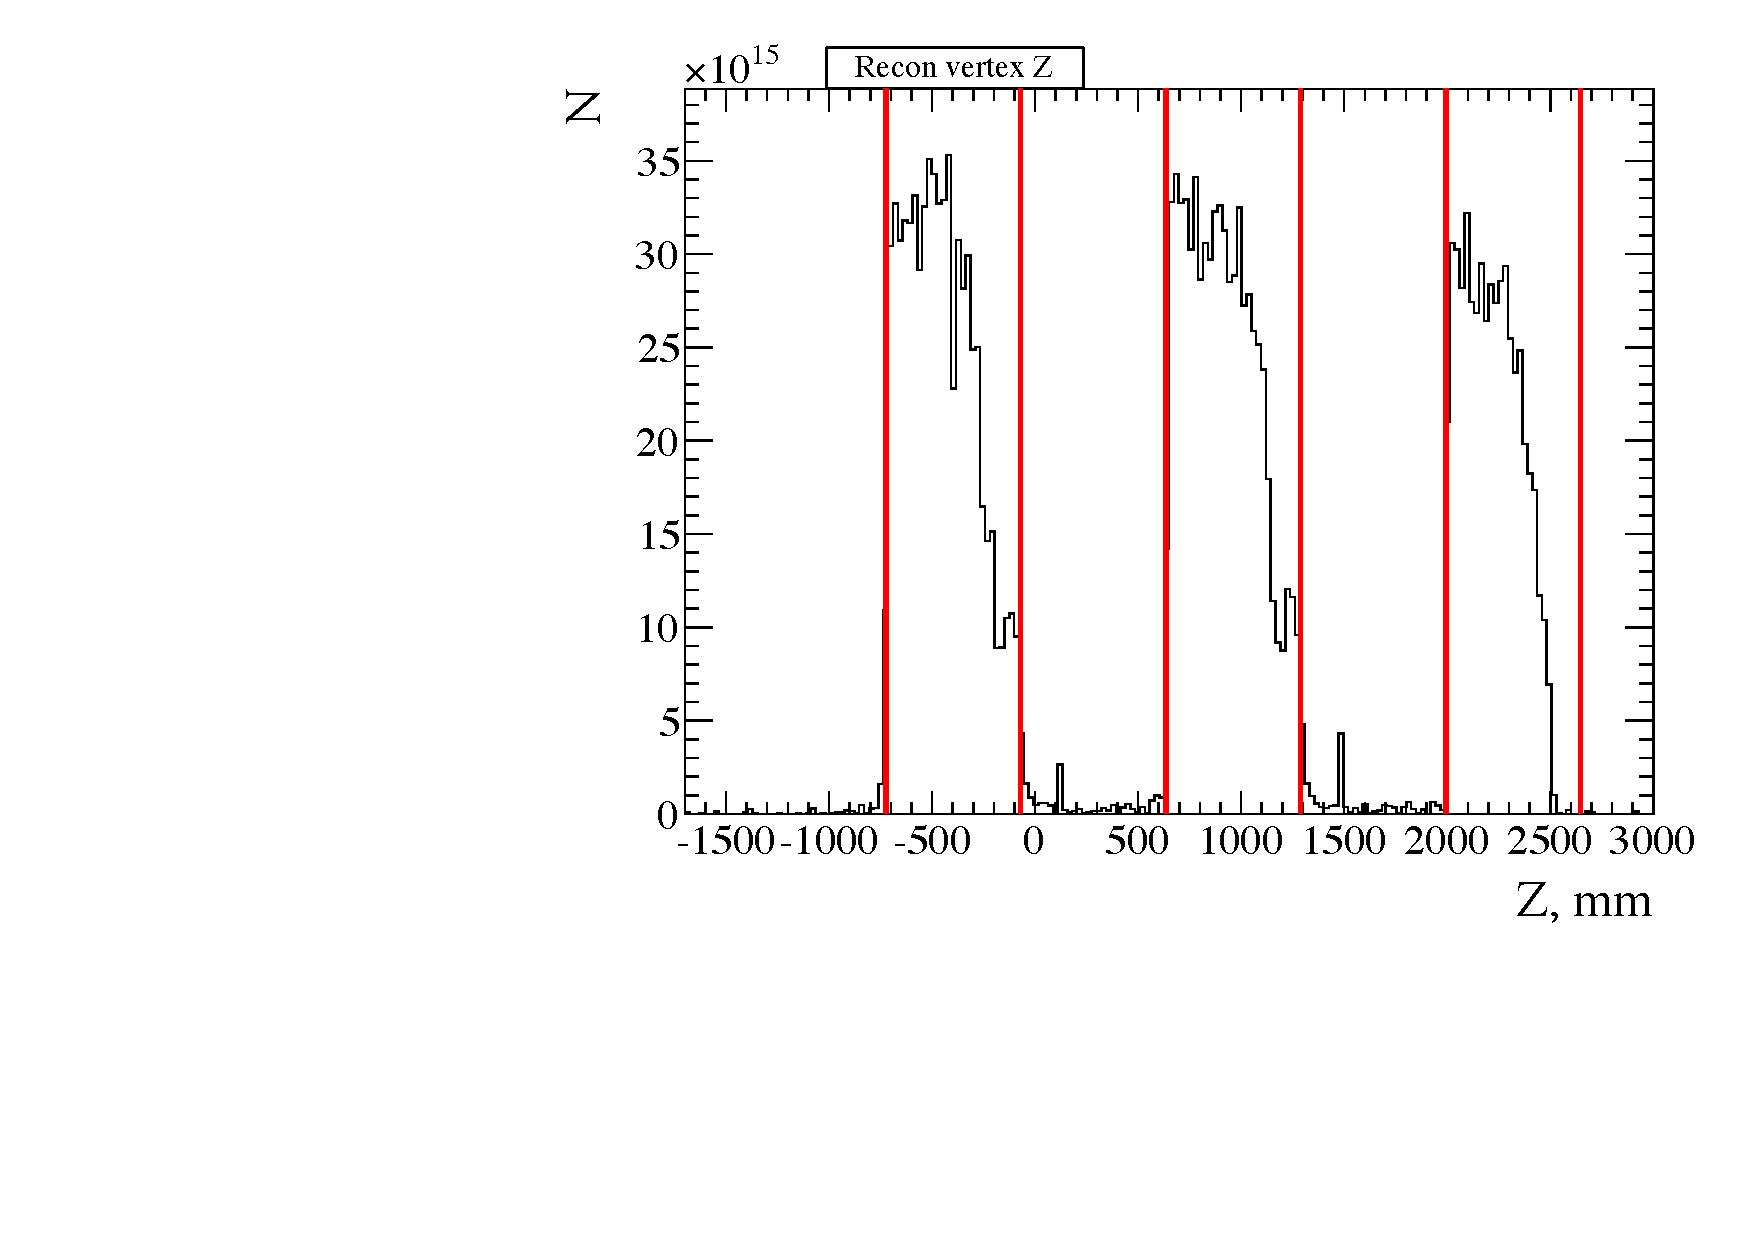
\includegraphics[width=0.7\linewidth]{vertexPos}}
  \caption{Vertex position for signal samples before the FV cut. Red lines are TPC bounds.}
  \label{fig:HNL:vertexPos}
\end{figure}

\subsubsection{Veto cuts}
Signal events from the HNL decay can't have any activity in the upstream detector. But there are some background events from a neutral particle decay or interaction. For example, $\pi^0$ decay into to photons and further production of the electron-positron pair. Also some mesons or baryons that can be produced in the active neutrino interactions and can cause production signal-like events. To suppress such events we should apply some constraints on the upstream activity. There is a possibility of electronics noises in the detector. Also there can be some activity after the previous bunch. To reduce event pile up we didn't constrict all the upstream activity. We developed the veto cut only for the first upstream detector. For the TPC1, we look for the P0D tracks which start or ends in the last P0D layers (100 mm). For the TPC2 and the  TPC3, we look at the FGD time bins. We are interested only in the bins that have a time signature near the center of bunch as this is only possibility to cause the vertex with two tracks in current bunch. Possible time gates are defined as $4\sigma$, where $\sigma=50ns$. The ``4 sigma'' is inherited from the default beam bunching procedure but the sigma value was increased as the bunch size for the massive neutrinos is larger (\autoref{sec:HNL:tof_corr}).

\subsubsection{HNL daughter-tracks start position}
Some cases of the vertex migration were found in the background analysis~(\autoref{sec:HNL:bg}). An active neutrino can interact in the FGD and all tracks of this event start in the FGD, but because of the errors of the reconstruction algorithm the vertex is extrapolated into the TPC FV. We can easily avoid such background with checking the activity in the TPC with vertex. If there are no tracks the event will be rejected.

\subsubsection{TPC additional activity cut}
Some process with more than two daughter particles can take place in the TPC. If only two of them are associated into the vertex the event will be signal-like. To prevent such background we apply the cut on the TPC activity. Only the HNL candidate daughters should start in the TPC with the vertex. If there is any additional track's start point the event is rejected.

\subsubsection{Particle identification}
We study the heavy neutrino decay into the charged lepton and pion. For the particle identification the standard TPC $dE/dx$ methods were applied~\cite{Abgrall2011}. For the analysis we choose the longest TPC segment as containing the most reliable information. Then the likelihood is build for each of the considered particle option: electron, muon, pion, proton. For particular particle selection we are constraining its likelihood and also limiting other hypothesis likelihoods to stay at the low value.

\subsubsection{Invariant mass cut}
As we search a decay of a massive particle into two charged particles, the invariant mass can be calculated. The upper bound on the mass of the HNL produced from the kaon decay is $M_{HNL}<M_K\approx500MeV$ and the lower bound is $M_{HNL}>M_\ell+M_\pi$. But the resolution of the invariant mass reconstruction should be taken into account. The resolution of our detector is shown in Fig.~\ref{fig:HNL:InvMass}. We accept $4\sigma$ difference from the true value and assume cut value 750 MeV for the $\mu\pi$ mode and 850 MeV for the $e\pi$ mode. The lower bound is strictly defined by the invariant mass calculation method ($M_\ell+M_\pi$). The cut value is set to 250 MeV for the $\mu\pi$ and 140 MeV for the $e\pi$. This cut help to reject the events from active neutrino interactions with high reconstructed invariant mass that certainly can not be the HNL decays.

\subsubsection{Kinematic cuts}
The heavy neutrinos from the kaon decays in the decay volume have a momentum collinear to the beam axis. So the momenta of the reconstructed HNL candidate should have rather small polar angle. This constraint can significantly reduce the background because the direction of the charged particles from the active neutrino interactions is quite isotropic. Since the HNL is a rather massive particle its daughter particles shouldn't have large opening angle. We have studied angular distribution for both the background and the signal samples. Firstly we studied the distribution of the polar angle of the HNL candidate for events that passed all previous cuts, as it is the most strict kinematic cut. Then we looked at the opening angle of the HNL candidate daughters. The results are presented in Fig.~\ref{fig:HNL:kin1},~\ref{fig:HNL:kin2}~and~\ref{fig:HNL:kin3}. For this plots we use the NEUT MC results with a statistics $6.5\cdot 10^{21} POT$. On these plots the background is normalized to $10^{21}POT$. The total signal is normalized to 1, only the shape of the signal distribution is important. It can't be normalized to any POT as it is proportional to mixing element. The cut value were set in order to maximize the sensitivity.

\begin{figure}[!ht]
  \begin{minipage}[h]{0.49\linewidth}
    \center{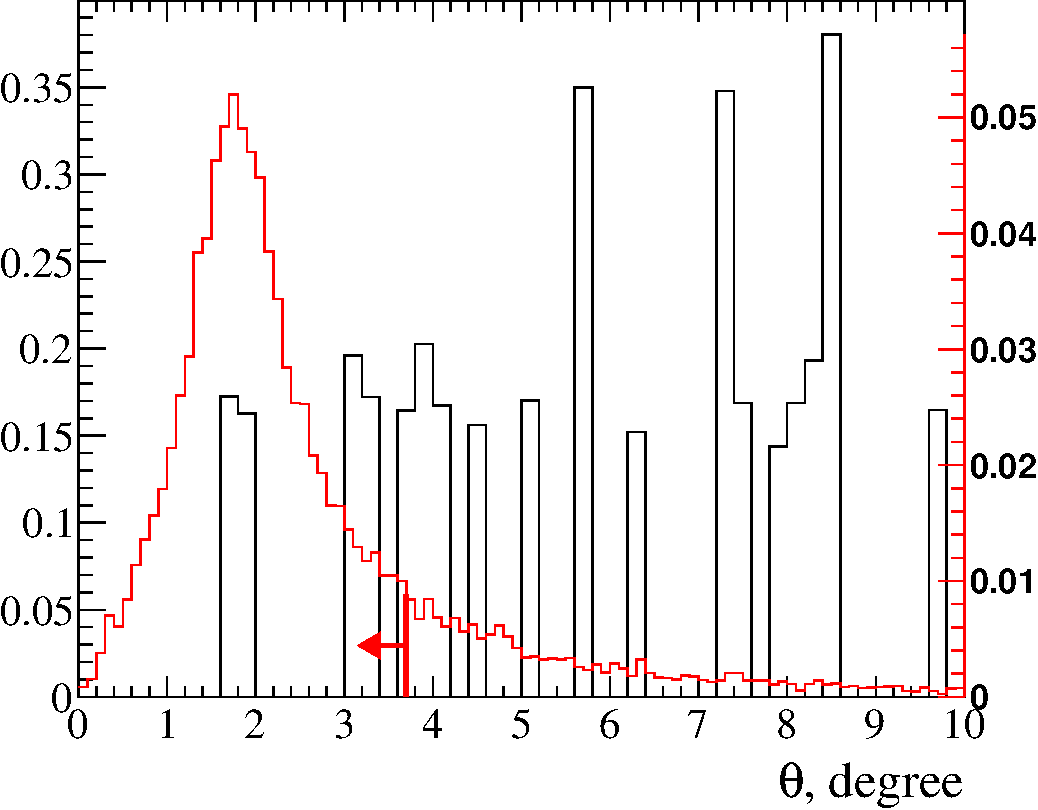
\includegraphics[width=\linewidth]{HNLpolarMu}  \\ a)}
  \end{minipage}
  \hfill
  \begin{minipage}[h]{0.49\linewidth}
    \center{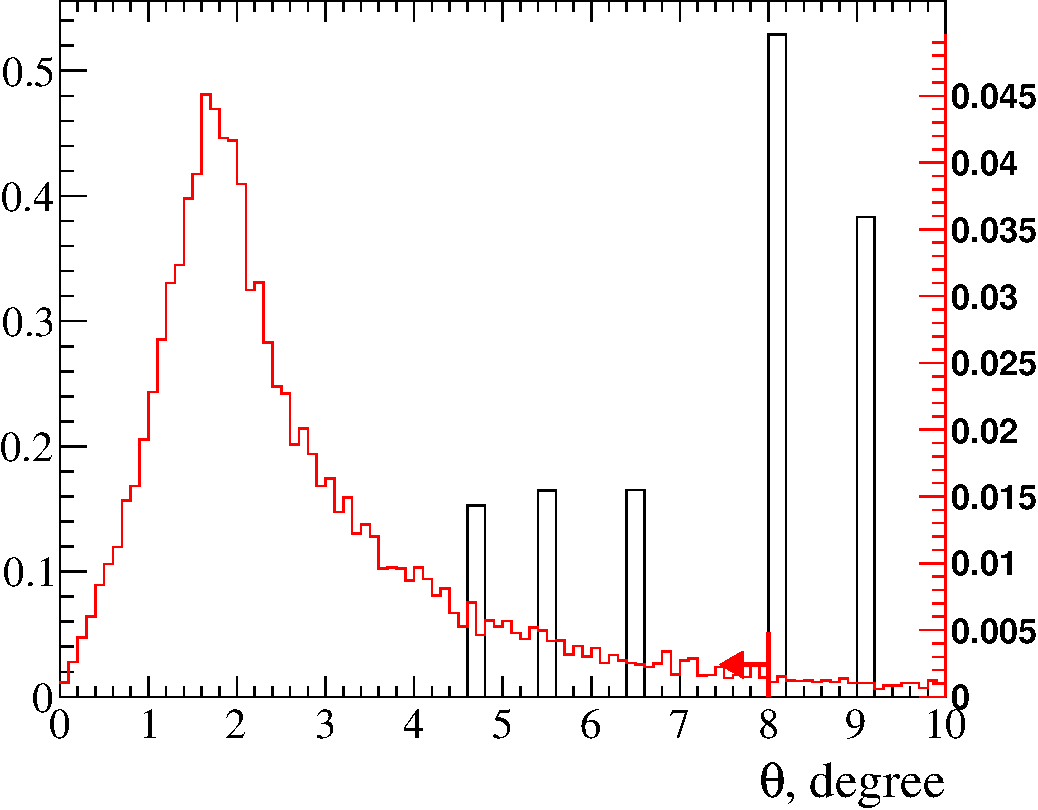
\includegraphics[width=\linewidth]{HNLpolarEle}  \\ b)}
  \end{minipage}
  \caption{Angular distribution of the HNL candidate events (a) for $\mu\pi$ mode and (b) for $e\pi$. Red is the signal samples, black is the BG and vertical line is a cut value. BG is normalized to $10^{21}POT$, signal is normalized to 1.}
  \label{fig:HNL:kin1}
\end{figure}

\begin{figure}[!ht]
  \center{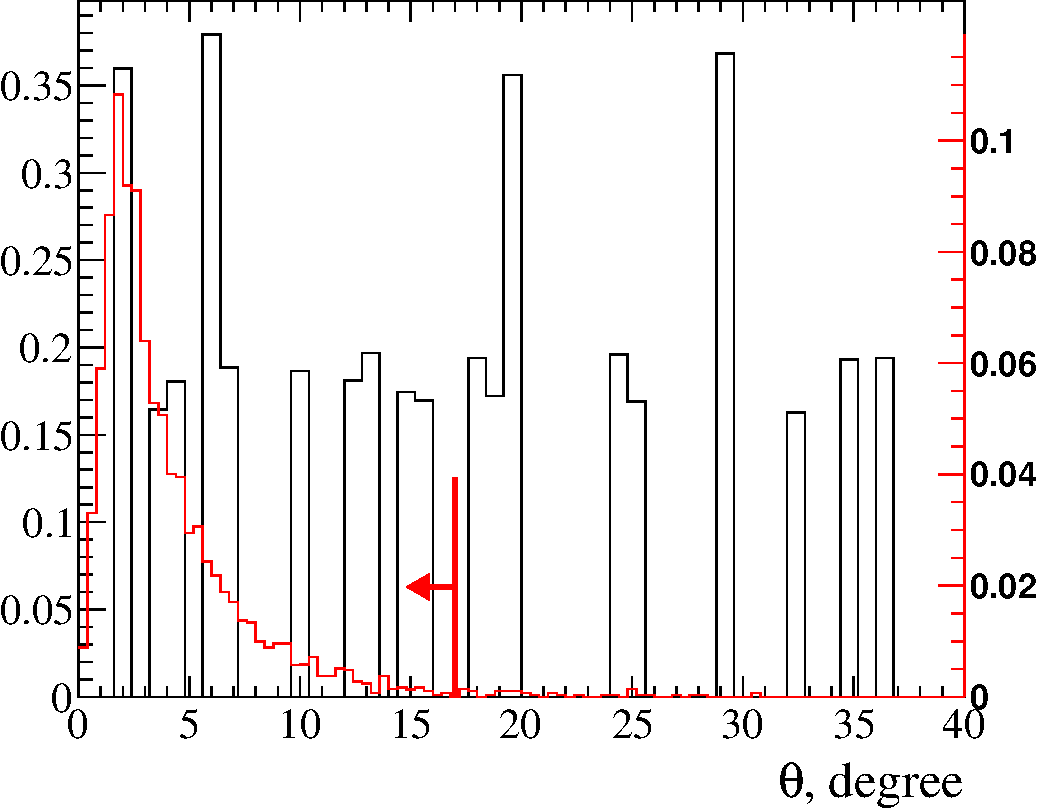
\includegraphics[width=0.5\linewidth]{HNLpolarDiMu}}
  \caption{Angular distribution of the HNL candidate events for $\mu\mu\nu$ mode. Red is the signal samples, black is the BG and vertical line is a cut value. BG is normalized to $10^{21}POT$, signal is normalized to 1.}
  \label{fig:HNL:kin2}
\end{figure}

\begin{figure}[!ht]
  \begin{minipage}[h]{0.49\linewidth}
    \center{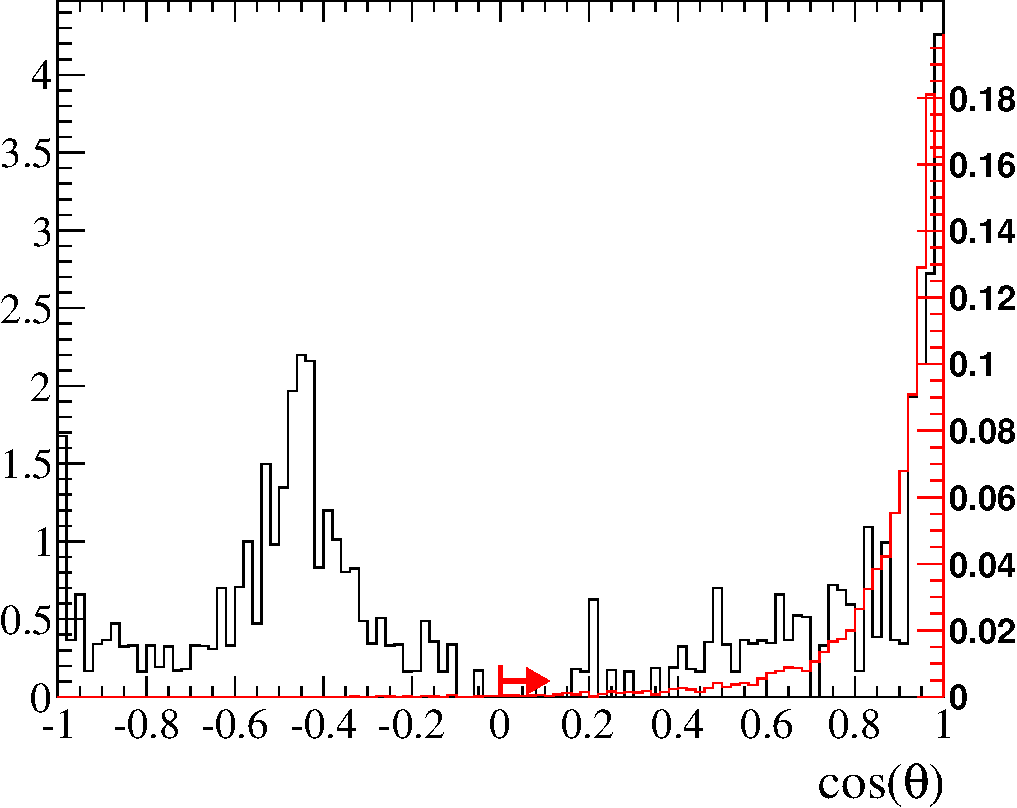
\includegraphics[width=\linewidth]{HNLrelative1} \\ a)}
  \end{minipage}
  \hfill
  \begin{minipage}[h]{0.49\linewidth}
    \center{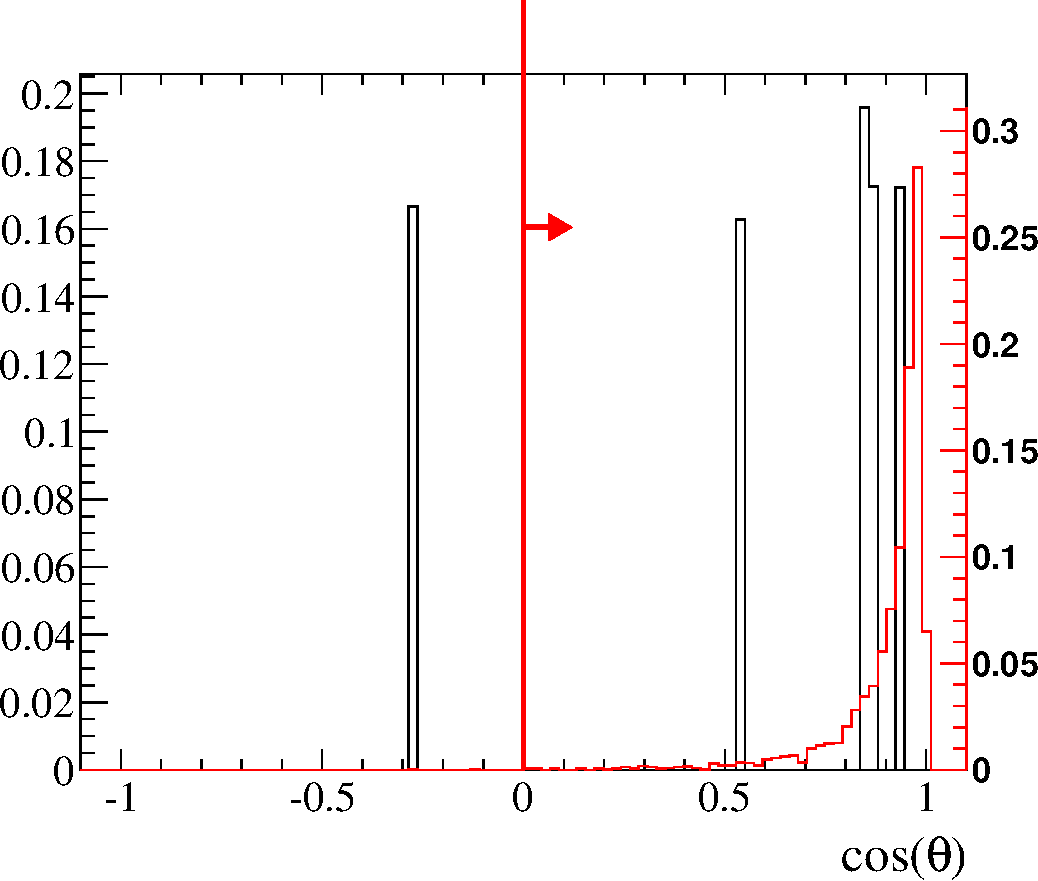
\includegraphics[width=\linewidth]{HNLrelative2} \\ b)}
  \end{minipage}
  \caption{An opening angle for the HNL daughter particles for the $\mu\pi$ mode (a) before the polar angle cut was applied and (b) after. Red is the signal samples, black is the BG and vertical line is a cut value. BG is normalized to $10^{21}POT$, signal is normalized to 1.}
  \label{fig:HNL:kin3}
\end{figure}

\subsubsection{\texorpdfstring{$N\to\mu\mu\nu$}{Lg}  mode cuts}
As we need to select only two muons, we should determine the particle type very accurately. The main problem is muon/pion separation in TPC. Also some protons can be identified as a muon with the $dE/dx$ method. As a muon has a high penetration ability, it is expected to reach the detectors outside the tracker. The protons have a very low probability to leave the tracker, so they will be rejected. The pions can leave the tracker but they will cause a shower in the ECal. For the pion/proton misidentification as a muon we select only events in which both muons' tracks have the subtracks in the ECal and these subtracks should be identified as MIP, but not as EM shower.

\subsection{Signal selection efficiency}
\label{sec:HNL:eff}

Applying all these cuts to the signal samples give us the total selection efficiency (\autoref{fig:HNL:Eff1}, \autoref{fig:HNL:Eff2}). The efficiency of the HNL selection in our TN is defined as a ratio of the number of the selected events to the number of the generated HNL events inside the TPCs FV. The main reason for the dependence of the efficiency on the HNL mass is the track reconstruction. For the large HNL mass we have more events with successfully reconstructed ``good quality'' tracks associated into the vertex.

\begin{figure}[!ht]
  \begin{minipage}{0.49\linewidth}
    \centering{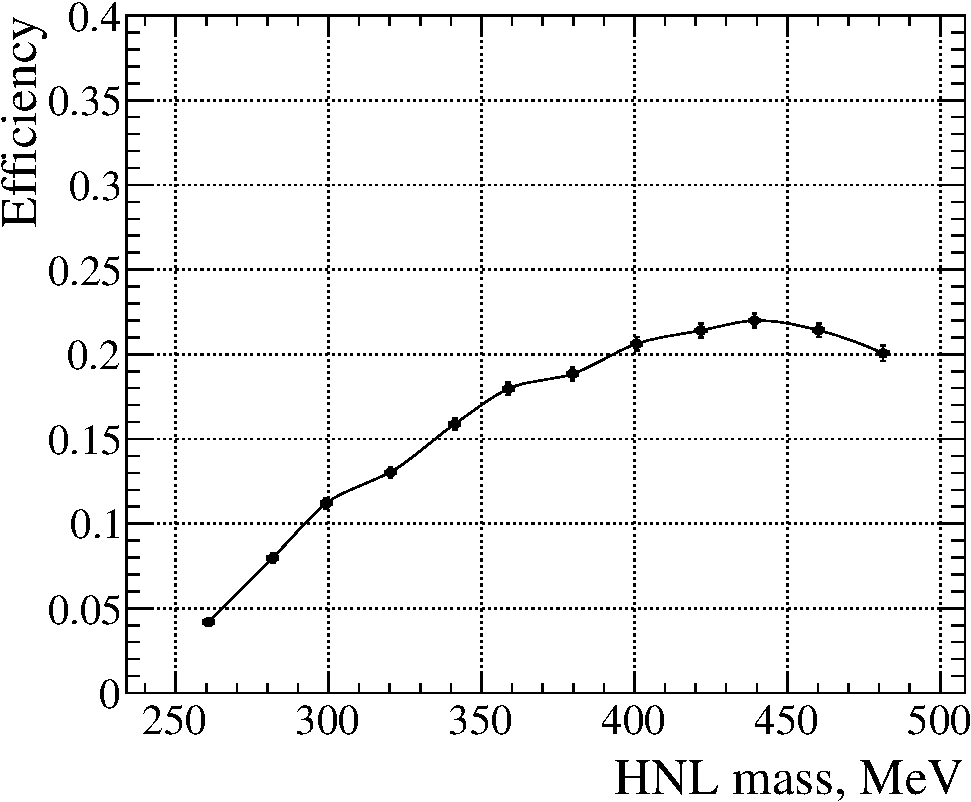
\includegraphics[width =\linewidth]{EffMu} \\ $K^+\to e^+N\to e^+\left(\mu^\mp\pi^\pm\right)$}
  \end{minipage}
  \hfill
  \begin{minipage}{0.49\linewidth}
    \centering{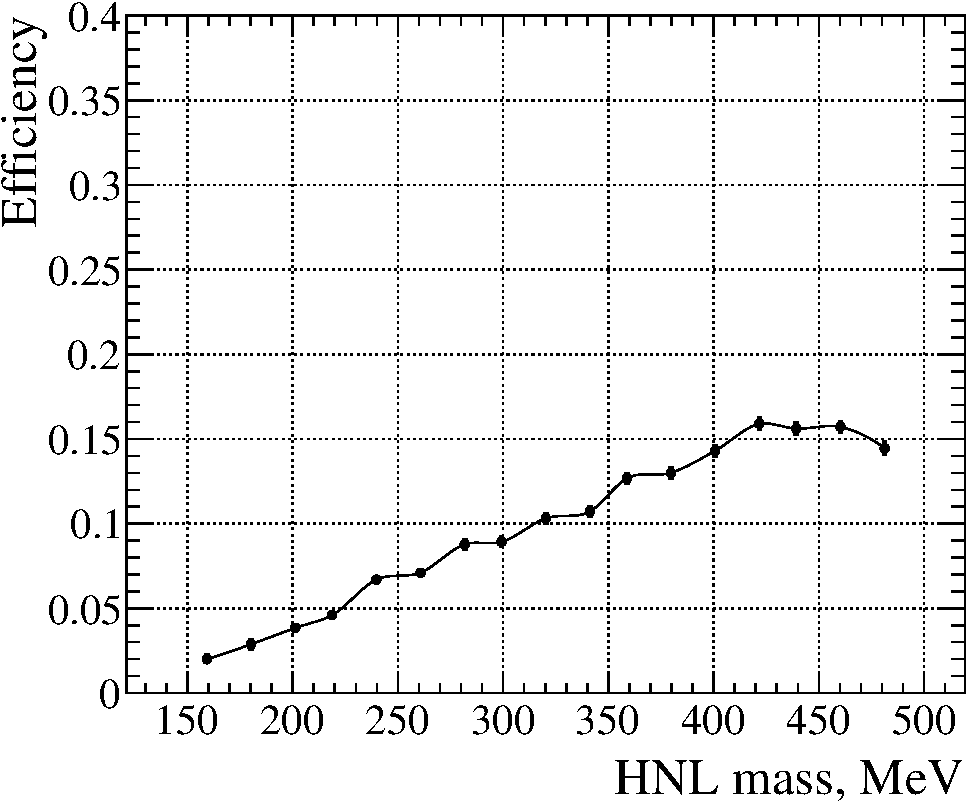
\includegraphics[width =\linewidth]{EffEle} \\ $K^+\to e^+N\to e^+\left(e^\mp\pi^\pm\right)$}
  \end{minipage}
  \caption{Selection efficiency for two body decays of HNL.}
  \label{fig:HNL:Eff1}
\end{figure}

\begin{figure}[!ht]
   \centering{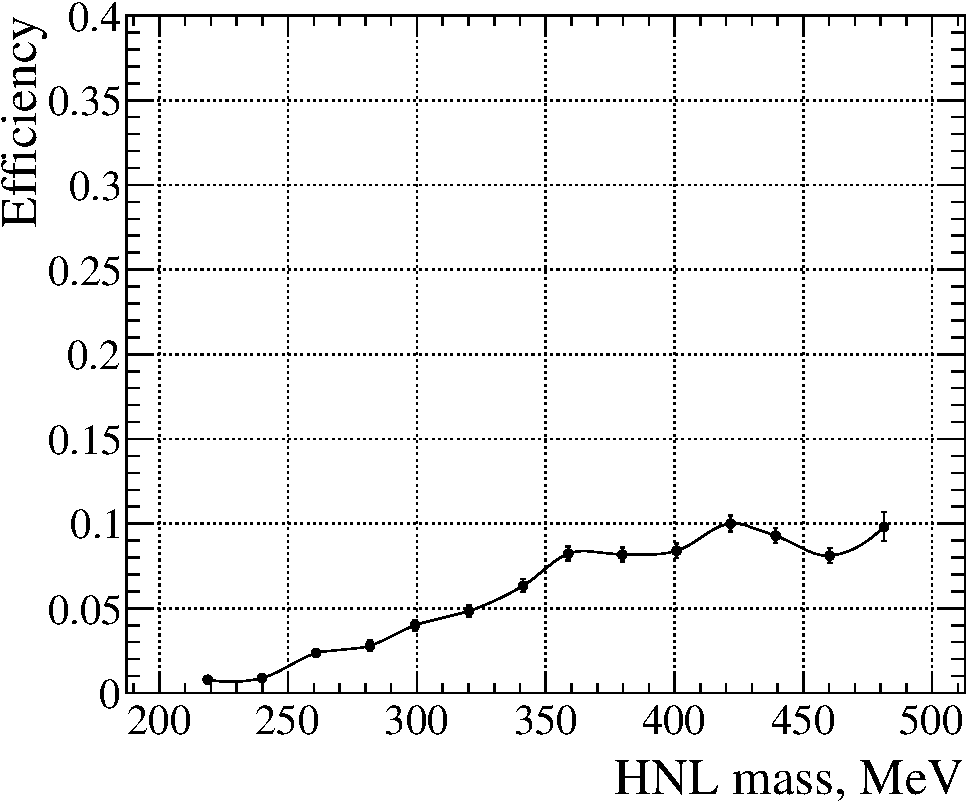
\includegraphics[width =0.4\linewidth]{EffDimuon}}
  \caption{Selection efficiency for HNL decay mode $N\to\mu\mu\nu$.}
  \label{fig:HNL:Eff2}
\end{figure}
The efficiency dependence on different cuts is shown in~\autoref{fig:HNL:EffDrop}. The main reason for the efficiency drop is ``quality and fiducial cut'' which is described in details in the~\autoref{sec:HNL:qf}.
\begin{figure}[!ht]
  \centering{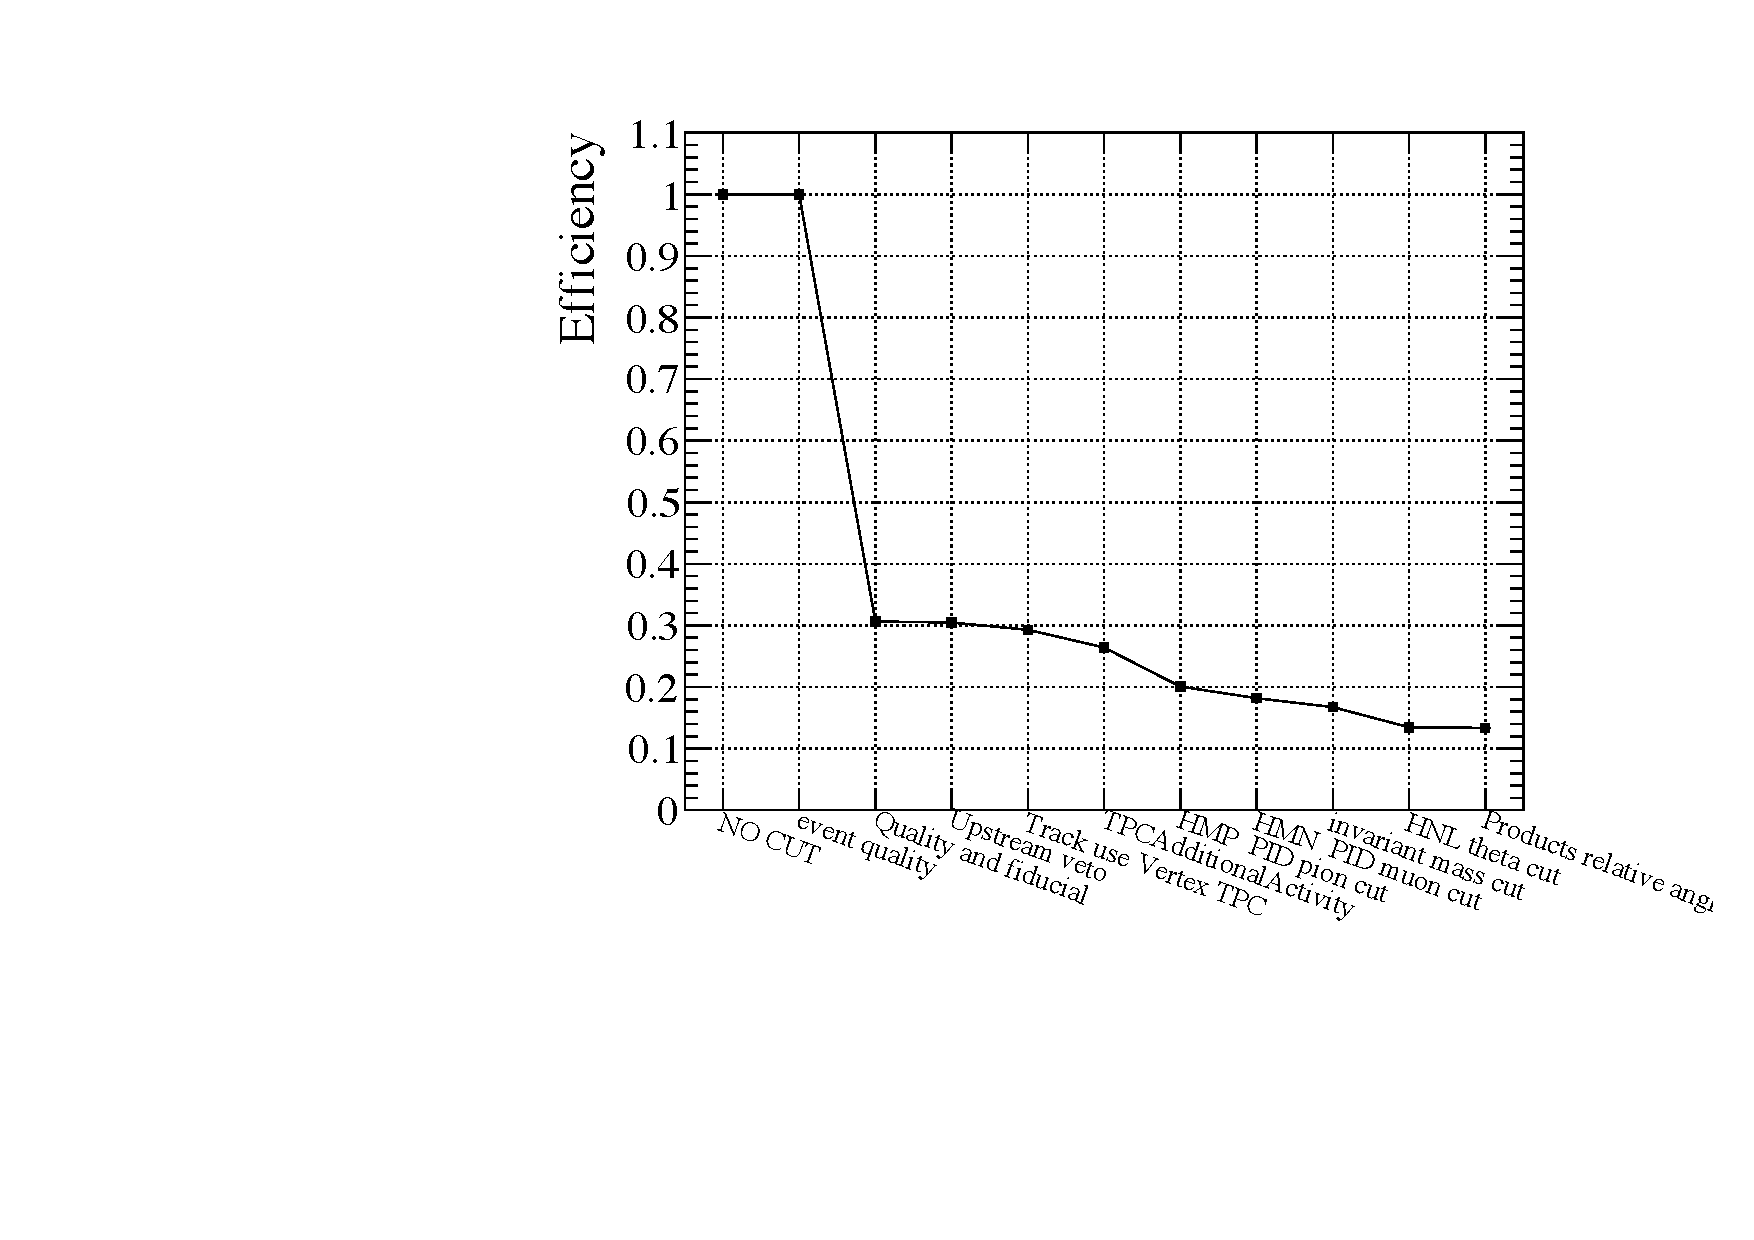
\includegraphics[width = 0.8\linewidth]{EffDrop}}
  \caption{Efficiency dependence on the applied cuts for mode $N\to\mu^\mp+\pi^\pm$ for all HNL masses.}
  \label{fig:HNL:EffDrop}
\end{figure}

The dependence of the efficiency on the HNL momentum and opening angle of the daughter particles is shown in~\autoref{fig:HNL:EffDep}. As expected the maximum efficiency is for HNL with momentum below 2 GeV. The TPCs were designed for the event reconstruction in this energy region.
\begin{figure}[!ht]
  \begin{minipage}{0.49\linewidth}
    \centering{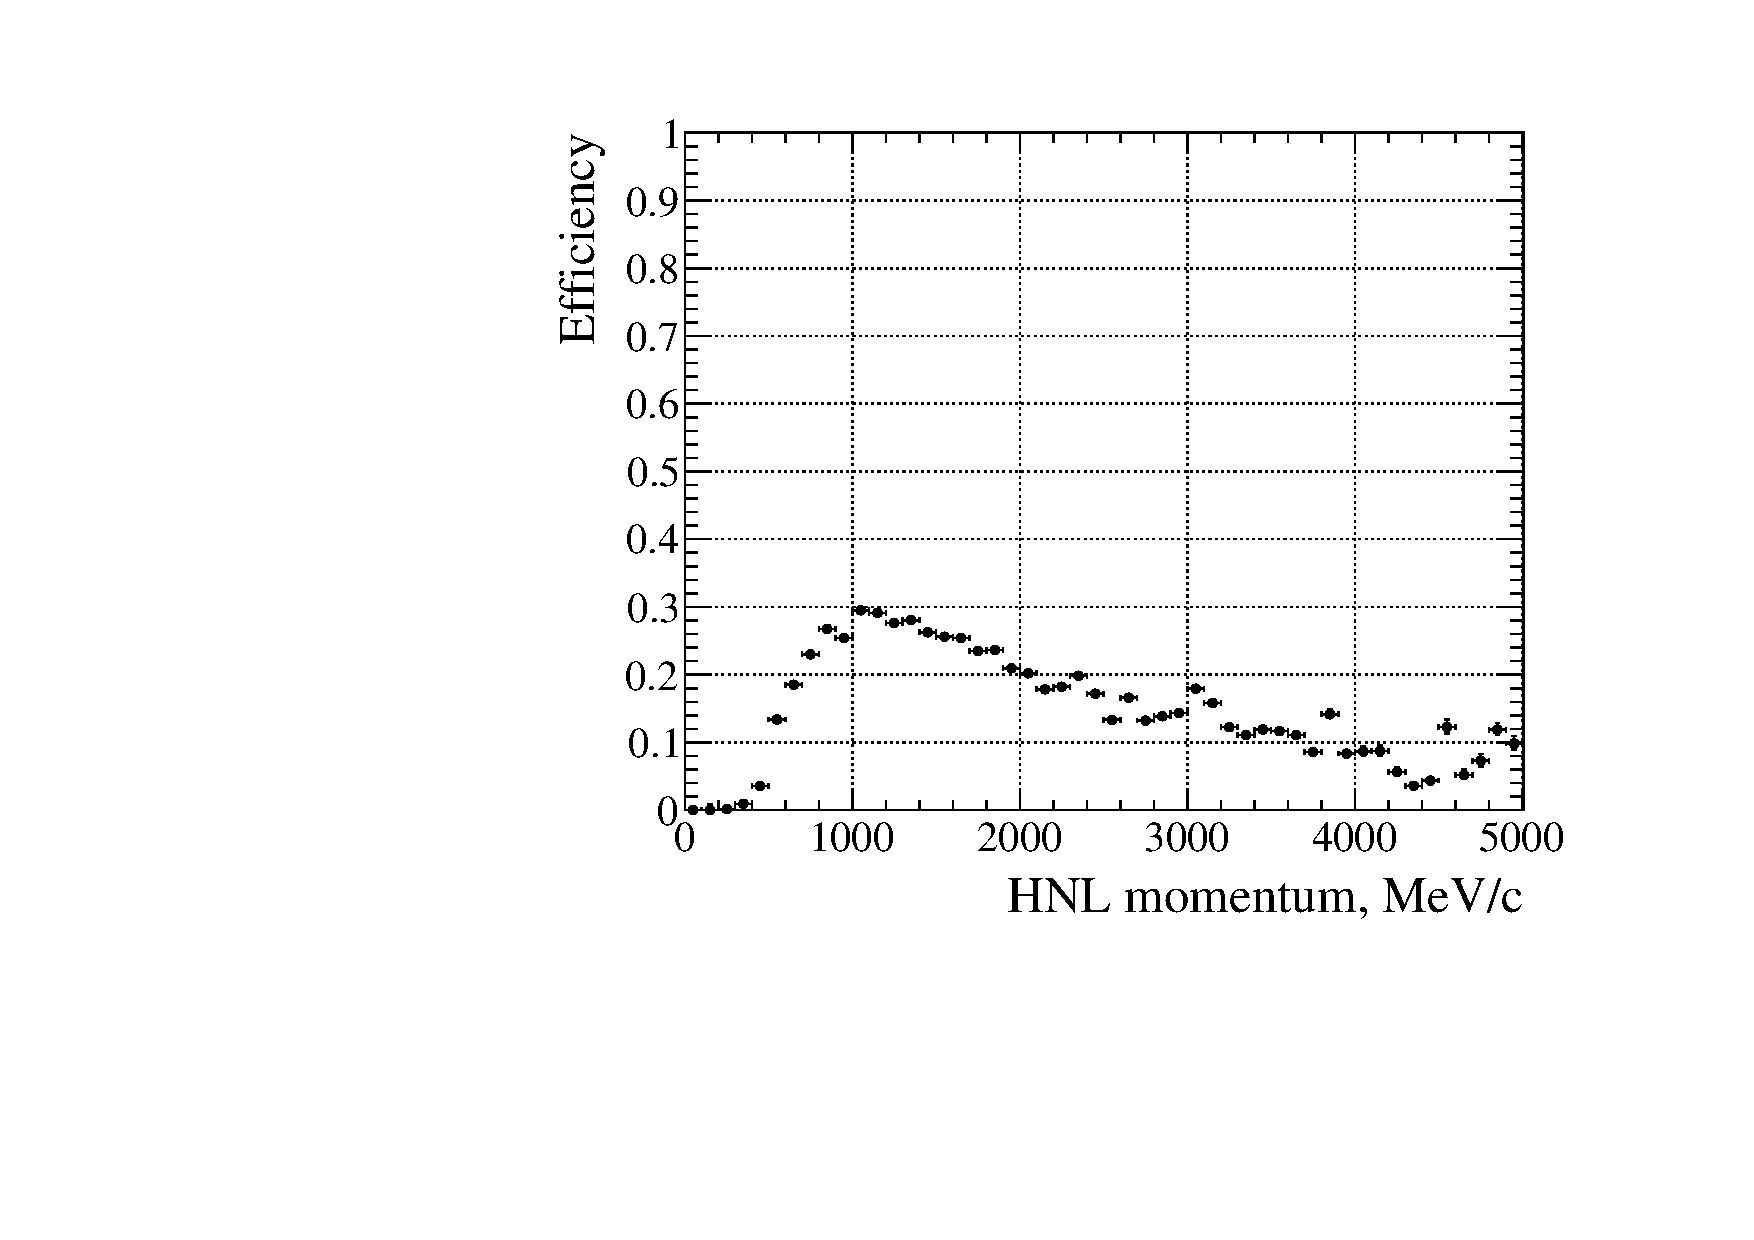
\includegraphics[width =\linewidth]{EffMom} \\ a)}
  \end{minipage}
  \hfill
  \begin{minipage}{0.49\linewidth}
    \centering{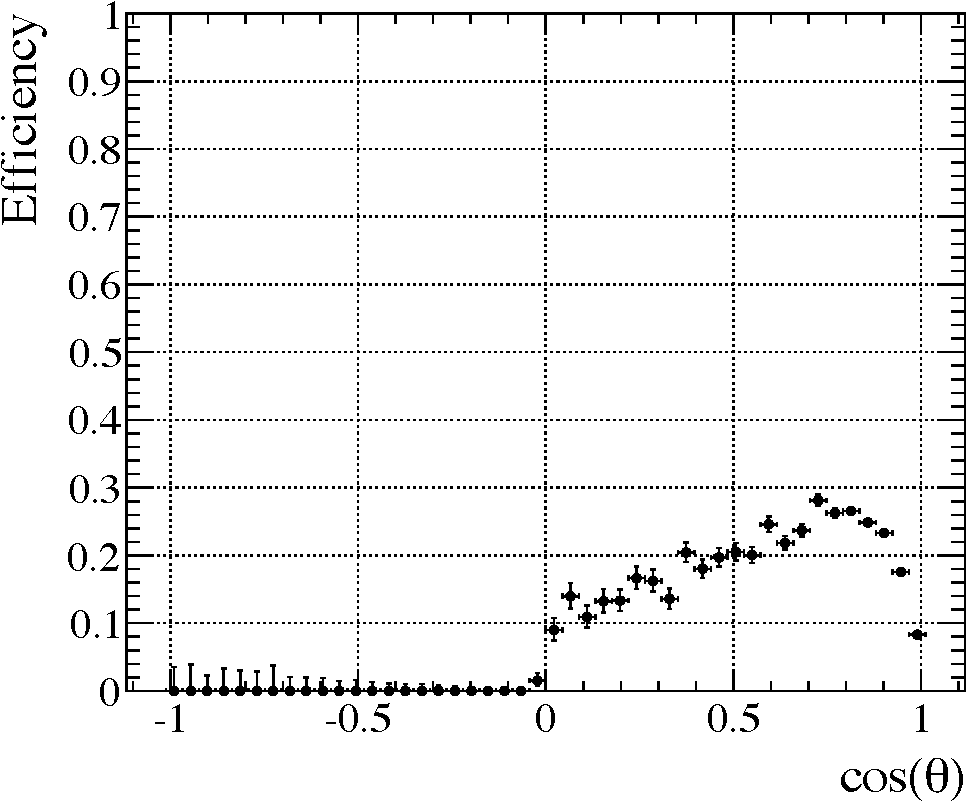
\includegraphics[width =\linewidth]{EffCos} \\ b)}
  \end{minipage}
  \caption{The dependence of efficiency for mode $N\to\mu\pi$: (a) on the HNL momentum and (b) opening angle of daughter particles.}
  \label{fig:HNL:EffDep}
\end{figure}

Since we study the HNL production from $K^+$,  $K^-$ and their decays into $\ell^{\pm}h^{\mp}$, the efficiency should be evaluated for each of them. Such result is presented in Fig.~\ref{fig:HNL:C_check}. We can see the agreement of the efficiency study for the different modes. The only difference is that the $\mu^-\pi^+$ selection efficiency is a bit higher than the $\mu^+\pi^-$ one.
\begin{figure}[!ht]
  \begin{minipage}{0.49\linewidth}
    \centering{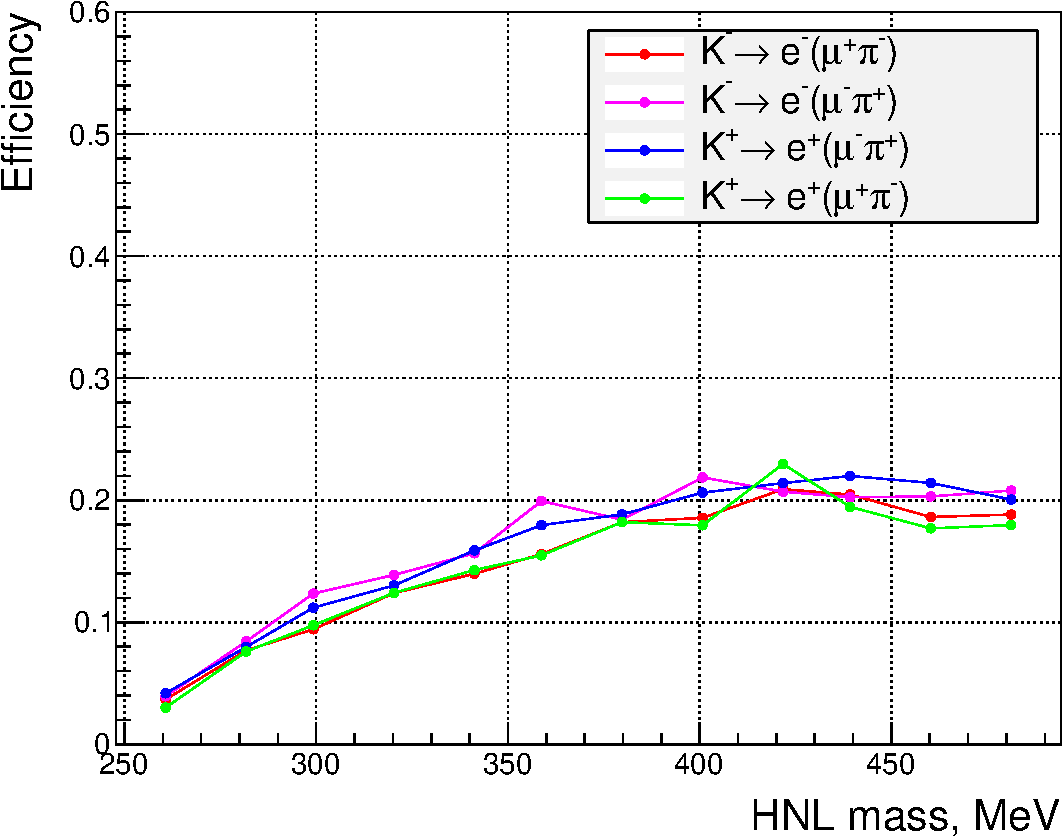
\includegraphics[width =\linewidth]{C_checkMu} \\ $N\to \mu\pi$}
  \end{minipage}
  \hfill
  \begin{minipage}{0.49\linewidth}
    \centering{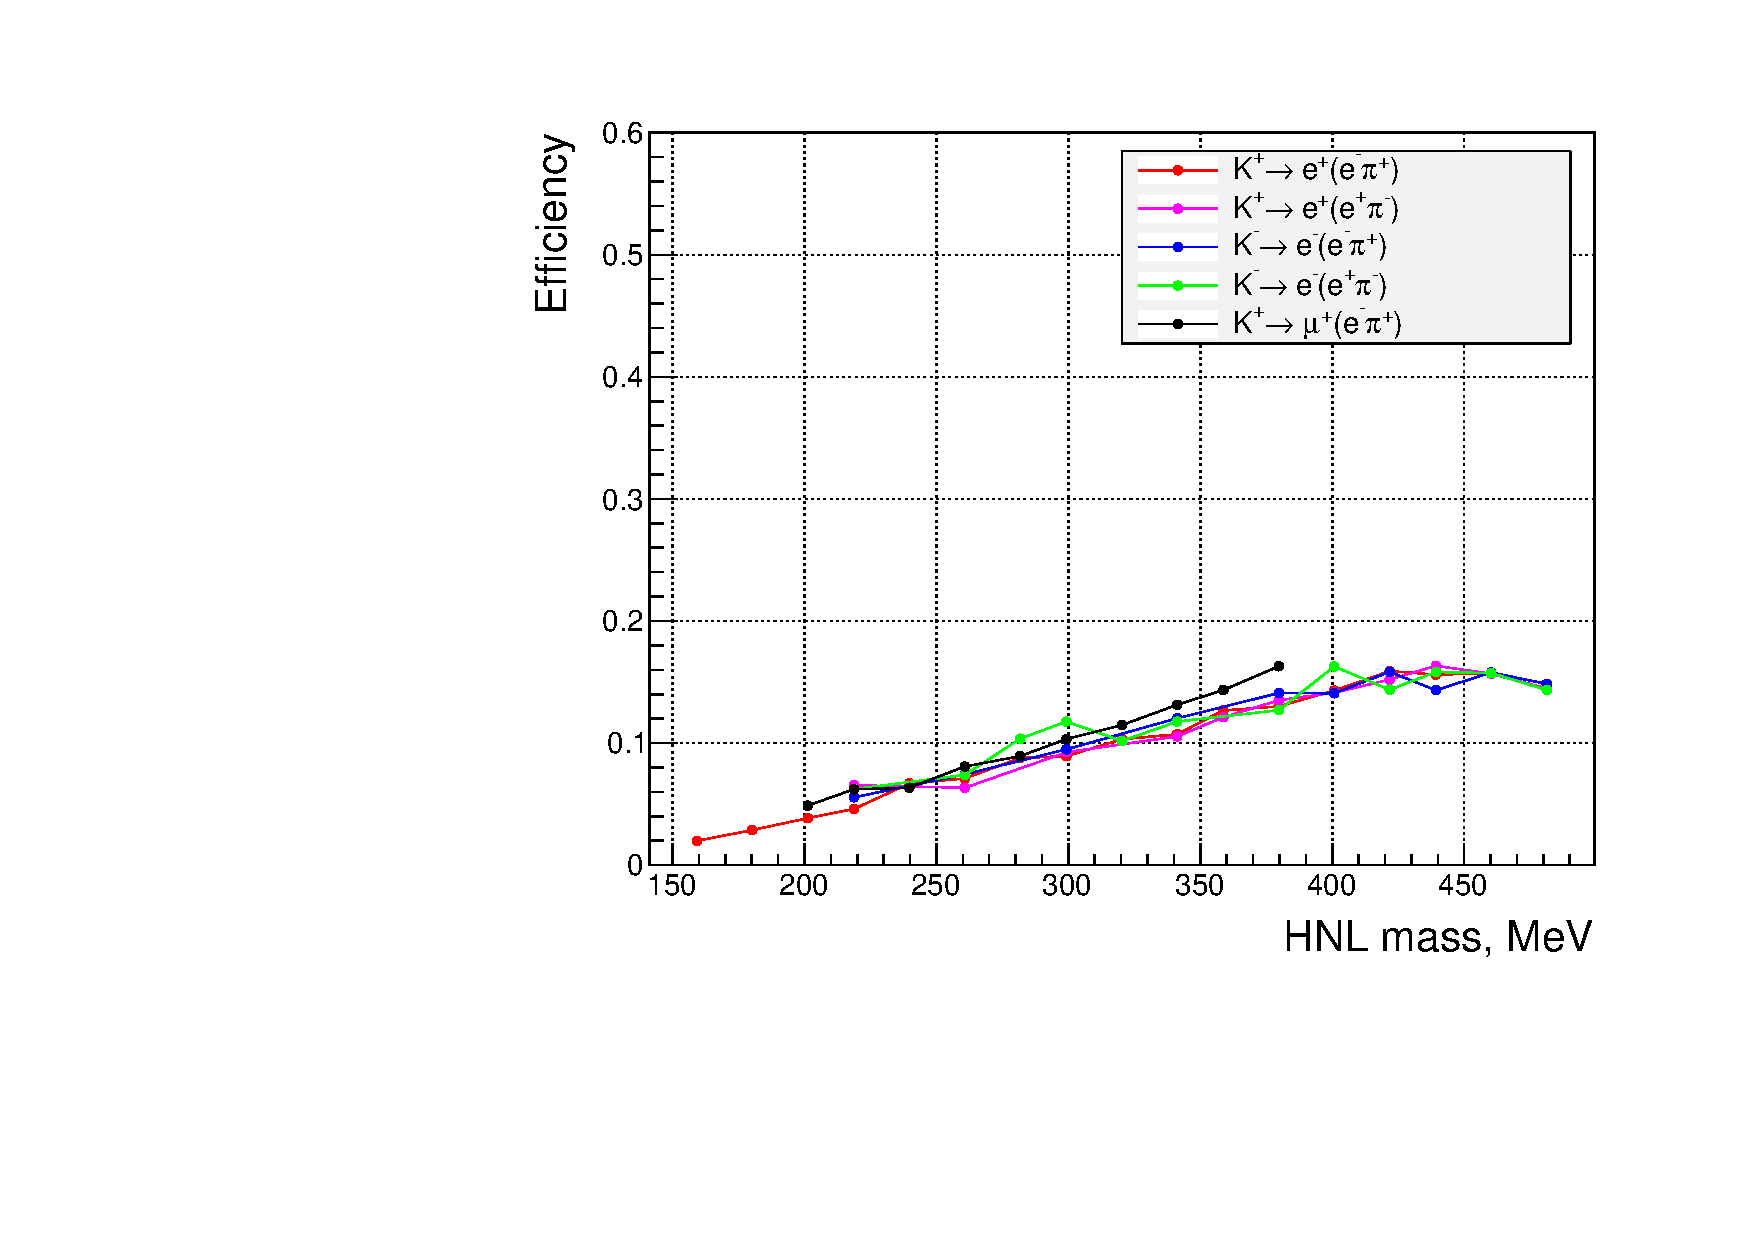
\includegraphics[width =\linewidth]{C_checkEle} \\ $N\to e\pi$}
  \end{minipage}
  \caption{HNL selection efficiencies for several production and decay modes.}
  \label{fig:HNL:C_check}
\end{figure}

\subsection{Background suppression}
\label{sec:HNL:bg}
Applying the same selection cuts to MC data from the different generators NEUT, GENIE and NuWro, we can estimate the background. We use different generators for the cross-check as they use slightly different neutrino interactions parameters. For example, Genie is more common for the kaon analysis (we can expect BG from $K^0$); NuWro gives a large statistic for the TPC volume. Following statistics was studied, for NEUT $6.5\cdot 10^{21} POT$, for GENIE $5\cdot 10^{21}POT$, for $\bar{\nu}$ mode with NEUT $5.8\cdot 10^{21}$. We studied the MC data from interaction in the magnet volume for NEUT and GENIE. NuWro provides data with neutrino interactions only in TPC volume with statistics $4.7\cdot10^{22}$, $4.76\cdot10^{22}$, $4.69\cdot10^{22}$ POT for TPC1, TPC2 and TPC3 respectively. OOFV (Out Of Fiducial Volume) processes are not simulated with the NuWro and few events identified as OOFV have true vertices in TPC but not in FV. For comparison of the background all the results were normalized to $10^{21}POT$. The efficiency of signal event selection and the background reduction for the different reaction types of active neutrino interactions based on run 2-6 from the NEUT generator are shown in~\autoref{tbl:HNL:bgOrigMu},~\autoref{tbl:HNL:bgOrigEle},~\autoref{tbl:HNL:bgOrigDiMuon}. The efficiency is equal for the same modes as we use our own HNL generator and the result does not depend on the neutrino generator. For more detailed cut description see Sec.~\ref{sec:HNL:sel}. The relative angle cut (kinematic) is shown in the table only if it reduces the number of the background events comparing to the polar angle cut.We start with the ``Quality and fiducial'' cut which requires  vertex with two different charge tracks in the TPC fiducial volume. Here we have the main efficiency drop down to ~50\% (\autoref{sec:HNL:qf}).

\begin{table}[!ht]
%\begin{adjustbox}{width=1.1\linewidth,center}
\begin{tabular}{|c|l|r|r|r|r|r|r|r|r|r|r|r|}
  \hline
  N & Cut           &  CCQE   &  RES  &  DIS  &  COH  &  NC  &  2P2H  &  OOFV  &$\bar{\nu_{\mu}}$& $\nu_{e}$ & Total  & Eff\\
  \hline
  1 & Vertex        & 140.11  & 30.88 & 20.34 & 4.57  & 8.48 & 1.65   & 647.31 & 2.39            &  3.63     & 859.34 & 44.0 \\
  \hline
  2 & Veto          & 136.47  & 27.86 & 17.58 & 4.25  & 8.15 & 1.65   & 514.72 & 2.10            &  3.45     & 716.23 & 43.9 \\
  \hline
  3 & Use TPC       & 135.77  & 27.31 & 17.19 & 4.25  & 8.15 & 1.48   & 505.18 & 2.10            &  3.45     & 704.88 & 41.9 \\
  \hline
  4 & TPC act.      & 122.44  & 21.24 & 10.75 & 3.89  & 6.55 & 0.82   & 281.47 & 1.80            &  2.43     & 451.39 & 39.1 \\
  \hline
  5 & PID 1         & 99.68   & 16.10 & 8.47  & 3.39  & 4.84 & 0.66   & 130.92 & 1.65            &  0.36     & 266.06 & 37.2 \\
  \hline
  6 & PID 2         & 5.08    & 5.51  & 5.60  & 2.03  & 1.25 & 0.00   & 48.64  & 1.37            &  0.19     &  69.66 & 31.3 \\
  \hline
  7 & Inv mass      & 0.83    & 3.52  & 2.17  & 1.67  & 0.90 & 0.00   & 43.17  & 0.92            &  0.00     &  53.18 & 29.2  \\
  \hline
  8 & $\theta$ cut  & 0.00    & 0.17  & 0.36  & 0.34  & 0.00 & 0.00   & 0.00   & 0.00            &  0.00     &  0.87  & 21.3 \\
  \hline
  9 & Kinematic     & 0.00    & 0.17  & 0.20  & 0.34  & 0.00 & 0.00   & 0.00   & 0.00            &  0.00     &  0.70  & 21.1 \\
    \hline

\end{tabular}
\caption{The number of MC background events after every cut for $10^{21} POT$ from NEUT for $\mu\pi$ mode.}
\label{tbl:HNL:bgOrigMu}
%\end{adjustbox}
\end{table}

\begin{table}[!ht]
%\begin{adjustbox}{width=1.1\linewidth,center}
\begin{tabular}{|c|l|r|r|r|r|r|r|r|r|r|r|r|}
  \hline
  N & Cut           &  CCQE   &  RES  &  DIS  &  COH  &  NC  &  2P2H  &  OOFV  &$\bar{\nu_{\mu}}$& $\nu_{e}$ & Total  & Eff\\
  \hline
  1 & Vertex        & 140.11  & 30.88 & 20.34 & 4.57  & 8.48 & 1.65   & 647.31 & 2.39            &  3.63     & 859.34 & 34.5 \\
  \hline
  2 & Veto          & 136.47  & 27.86 & 17.58 & 4.25  & 8.15 & 1.65   & 514.72 & 2.10            &  3.45     & 716.23 & 34.4 \\
  \hline
  3 & Use TPC       & 135.77  & 27.31 & 17.19 & 4.25  & 8.15 & 1.48   & 505.18 & 2.10            &  3.45     & 704.88 & 33.6 \\
  \hline
  4 & TPC act.      & 122.44  & 21.24 & 10.75 & 3.89  & 6.55 & 0.82   & 281.47 & 1.80            &  2.43     & 451.39 & 31.1 \\
  \hline
  5 & PID 1         & 99.68   & 16.10 & 8.47  & 3.39  & 4.84 & 0.66   & 130.92 & 1.65            &  0.36     & 266.06 & 24.8 \\
  \hline
  6 & PID 2         & 5.74    & 0.17  & 0.92  & 0.17  & 0.20 & 0.00   & 13.91  & 0.00            &  0.00     &  21.11 & 17.8 \\
  \hline
  7 & Inv mass      & 0.66    & 0.17  & 0.37  & 0.17  & 0.20 & 0.00   & 13.32  & 0.00            &  0.00     &  14.87 & 17.1  \\
  \hline
  8 & $\theta$ cut  & 0.00    & 0.00  & 0.00  & 0.17  & 0.00 & 0.00   & 0.32   & 0.00            &  0.00     &  0.48  & 15.2 \\
  \hline
  9 & Kinematic     & 0.00    & 0.00  & 0.00  & 0.17  & 0.00 & 0.00   & 0.32   & 0.00            &  0.00     &  0.48  & 14.8 \\
    \hline

\end{tabular}
\caption{The number of MC background events after every cut for $10^{21} POT$ from NEUT for $e\pi$ mode.}
\label{tbl:HNL:bgOrigEle}
%\end{adjustbox}
\end{table}

\begin{table}[!ht]
%\begin{adjustbox}{width=1.1\linewidth,center}
\begin{tabular}{|c|l|r|r|r|r|r|r|r|r|r|r|r|}
  \hline
  N & Cut           &  CCQE   &  RES  &  DIS  &  COH  &  NC  &  2P2H  &  OOFV  &$\bar{\nu_{\mu}}$& $\nu_{e}$ & Total  & Eff\\
  \hline
  1 & Vertex        & 140.11  & 30.88 & 20.34 & 4.57  & 8.48 & 1.65   & 647.31 & 2.39            &  3.63     & 859.34 & 42.1 \\
  \hline
  2 & Veto          & 136.47  & 27.86 & 17.58 & 4.25  & 8.15 & 1.65   & 514.72 & 2.10            &  3.45     & 716.23 & 42.0 \\
  \hline
  3 & Use TPC       & 135.77  & 27.31 & 17.19 & 4.25  & 8.15 & 1.48   & 505.18 & 2.10            &  3.45     & 704.88 & 40.5 \\
  \hline
  4 & TPC act.      & 122.44  & 21.24 & 10.75 & 3.89  & 6.55 & 0.82   & 281.47 & 1.80            &  2.43     & 451.39 & 38.2 \\
  \hline
  5 & PID 1         & 121.90  & 17.97 & 9.27  & 3.54  & 4.19 & 0.82   & 134.29 & 1.36            &  0.54     & 284.87 & 33.6 \\
  \hline
  6 & PID 2         & 4.38    & 5.01  & 5.22  & 1.70  & 0.91 & 0.00   & 27.59  & 1.08            &  0.91     &  46.09 & 22.5 \\
  \hline
  7 & Use ECal      & 2.12    & 1.79  & 1.89  & 0.68  & 0.34 & 0.00   & 2.56   & 0.33            &  0.00     &  9.72  &  9.9  \\
  \hline
  8 & ECal MIP      & 1.09    & 0.55  & 1.31  & 0.51  & 0.00 & 0.00   & 1.08   & 0.16            &  0.00     &  4.71  &  9.3  \\
  \hline
  9 & $\theta$ cut  & 0.93    & 0.36  & 0.39  & 0.51  & 0.00 & 0.00   & 0.00   & 0.00            &  0.00     & 2.18   &  9.1 \\
  \hline

\end{tabular}
\caption{The number of MC background events after every cut for $10^{21} POT$ from NEUT for $\mu\mu\nu$ mode.}
\label{tbl:HNL:bgOrigDiMuon}
%\end{adjustbox}
\end{table}

Finally we have:

\begin{table}[!ht]
\begin{center}
\begin{tabular}{lllll}
                              & NEUT                    & GENIE                   & NuWro               & NEUT $\bar{\nu}$  \\
  $\mu\pi$ \hspace{0.5cm}     & 0.79   \hspace{1cm}     & 0.69  \hspace{1cm}      & 0.85  \hspace{1cm}  & 0.91              \\
  $e\pi$                      & 0.69                    & 0.95                    & 0.38                & 0.23              \\
  $\mu\mu\nu$                 & 1.81                    & 1.63                    & 2.10                & 0.98              \\
\end{tabular}
\caption{The total number of MC background events for $10^{21} POT$.}
\label{tbl:HNL:bg}
\end{center}
\end{table}

As one can see, the different generators give nearly the same results. The reduction of background for mode $e\pi$ with NuWro generator caused by the lack of the data with neutrino events outside TPC --- on of the most influential BG process. For our estimations we take the worse result --- the maximum background.

The statistics accumulated in the T2K experiment is divided into 8 runs. The total good quality data available for analysis is $\left(10.23\nu+6.29\bar{\nu}\right)\cdot 10^{20}POT$. Scaling of the MC backgrounds to the real data, collected at ND280, gives us the expected number of the background events (Table~\ref{tbl:HNL:bgScale}).

\begin{table}[!ht]
\begin{center}
\begin{tabular}{llll}
                            & run 2-8               \\
  $\mu\pi$ \hspace{0.5cm}   & 1.44  \hspace{2cm}    \\
  $e\pi$                    & 1.12                  \\
  $\mu\mu\nu$               & 2.85                  \\
\end{tabular}
\caption{The total number of MC background events scaled to real data statistics.}
\label{tbl:HNL:bgScale}
\end{center}
\end{table}

The origin of the backgrounds for $N\to\mu\pi$ mode is interactions in gas, mainly coherent and resonance pion production. For the $N\to e\pi$ mode the main background process is $\pi^0$ decay into two gammas and further electron positron pair production and misreconstruction one of the pair component as a pion. For the $\mu\mu\nu$ mode the main background is CCQE. We select tracks for the muon candidates with ECal. The candidate should be MIP like so pions from the COH and RES processes are suppressed. But the protons that were misidentified as a muon in TPC can give a track in ECal. Such tracks can be reconstructed as MIP in some cases.

Neutrino interactions in gas were not well studied and it leads to the large uncertainties of the background estimation. So, we are going this MC data only for comparison with the real data, but not for the final result estimation. This strategy was described in~\autoref{sec:HNL:stat}.

\section{Systematic uncertainties}
\label{sec:HNL:sys}
In general case the systematic uncertainty will come both from the signal expectations and from the estimations background. In our case (\autoref{sec:HNL:stat}) the background estimations are not affecting the final sensitivity result. Thus their systematics could be omitted.

In this case we have the systematic uncertainties only from the number of predicted events. Assuming $\left|U\right|^2=1$ we calculated the events number according to \autoref{eq:HNL:Nevents}
\begin{equation}
  N_{events}=\phi(HNL/10^{21}p.o.t./cm^2)\cdot\frac{V_{FV}}{c\beta\gamma}\cdot\Gamma_{mode}\cdot Eff,
\end{equation}
where $Eff$ is the selection efficiency. Possible uncertainties sources are:
\begin{itemize}
  \item $\phi(HNL/10^{21}p.o.t./cm^2)$ - a HNL flux. As it is calculated based on the kaon flux, the uncertainties of the kaon flux modeling should be included here,
  \item $Eff$ - a selection efficiency uncertainties, the detector systematics should be included here.
\end{itemize}

\subsection{Detector systematics}
To study detector uncertainties, we can use the results of the same study for the active neutrino interactions. But some changes should be applied as we use TPC instead of FGD. We consider the following systematics:
\begin{itemize}
    \item Magnetic Field distortions. Uncertainties in magnetic field map,
    \item TPC momentum scale,
    \item TPC momentum resolution,
    \item TPC PID. Uncertainties in particle identification,
    \item TPC tracking efficiency,
    \item TPC charge ID efficiency. Uncertainties of charge identification,
    \item TPC-FGD matching efficiency,
    \item TPC cluster efficiency. Additional inefficiency of TPC cluster reconstruction,
    \item Pion secondary interactions,
    \item Global vertex association
\end{itemize}

For the mode $N\to\mu\mu\nu$ we should consider additional ECal systematics as we use this detector in our cut sequence:

\begin{itemize}
    \item TPC-ECal track clustering and matching efficiency,
    \item ECal Particle Identification
\end{itemize}

\todo{put a comment about weight and variation systematics}


The systematic that was estimated by ourselves for this particular analysis is the uncertainty of the track association into the global vertex (GV). We look at the GV in the TPC fiducial volume. So we should estimate the vertex association systematics. It's impossible for neutrino interactions in the TPC FV because of the lack of the statistics, so the FGD FV was chosen for this study.

We check the efficiency of the successful association of the ``suitable'' tracks in vertex. Two samples are defined for the FGD1 and FGD2 respectively. ``Suitable'' means that the tracks should pass the following cuts:
\begin{itemize}
    \item both start in the FGD1/2 FV;
    \item different charge;
    \item close start position 50 mm for X and Y axis and 100 mm for Z axis;
    \item only one sample (FGD1 or FGD2) was filled with tracks that passed upper cuts.
\end{itemize}
The efficiency of the vertex merger is defined as the ratio of the number of the tracks' pairs associated in vertex to tracks' pairs that passed the cuts that were listed above. We should check if this efficiency depends on the tracks parameters i.e. momentum, opening angle. The results are presented in~\autoref{fig:HNL:GVsysDEP}
\begin{figure}[!ht]
    \begin{minipage}[h]{0.49\linewidth}
        \center{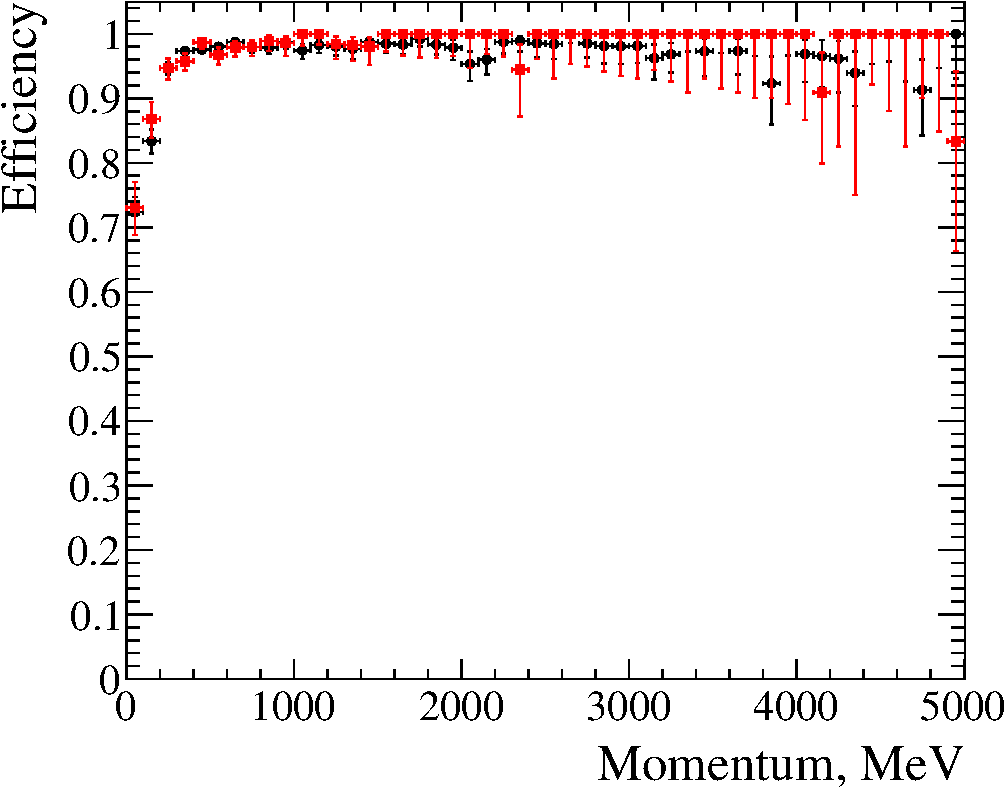
\includegraphics[width=\linewidth]{MomWide}}
    \end{minipage}
    \hfill
    \begin{minipage}[h]{0.49\linewidth}
        \center{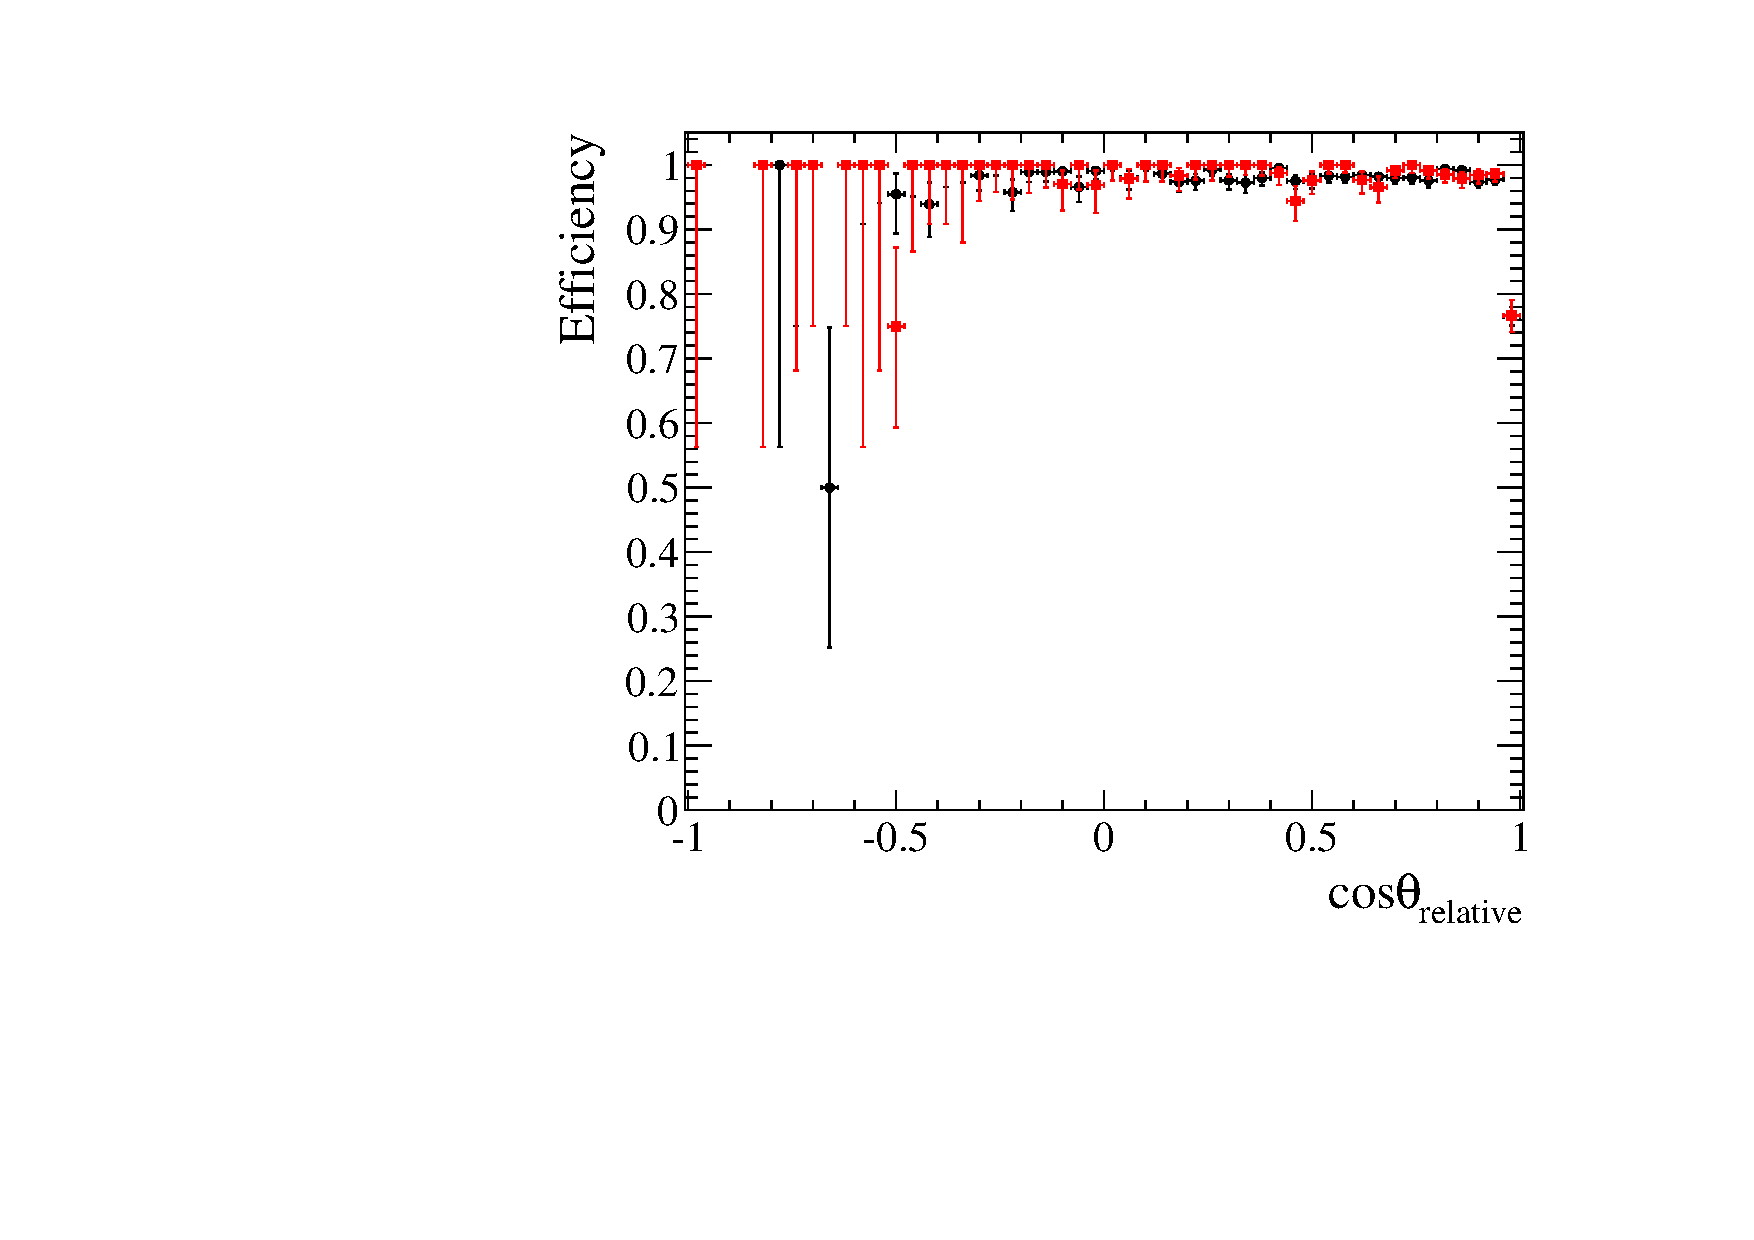
\includegraphics[width=\linewidth]{CosWide}}
    \end{minipage}
    \vfill
    \begin{minipage}[h]{0.49\linewidth}
        \center{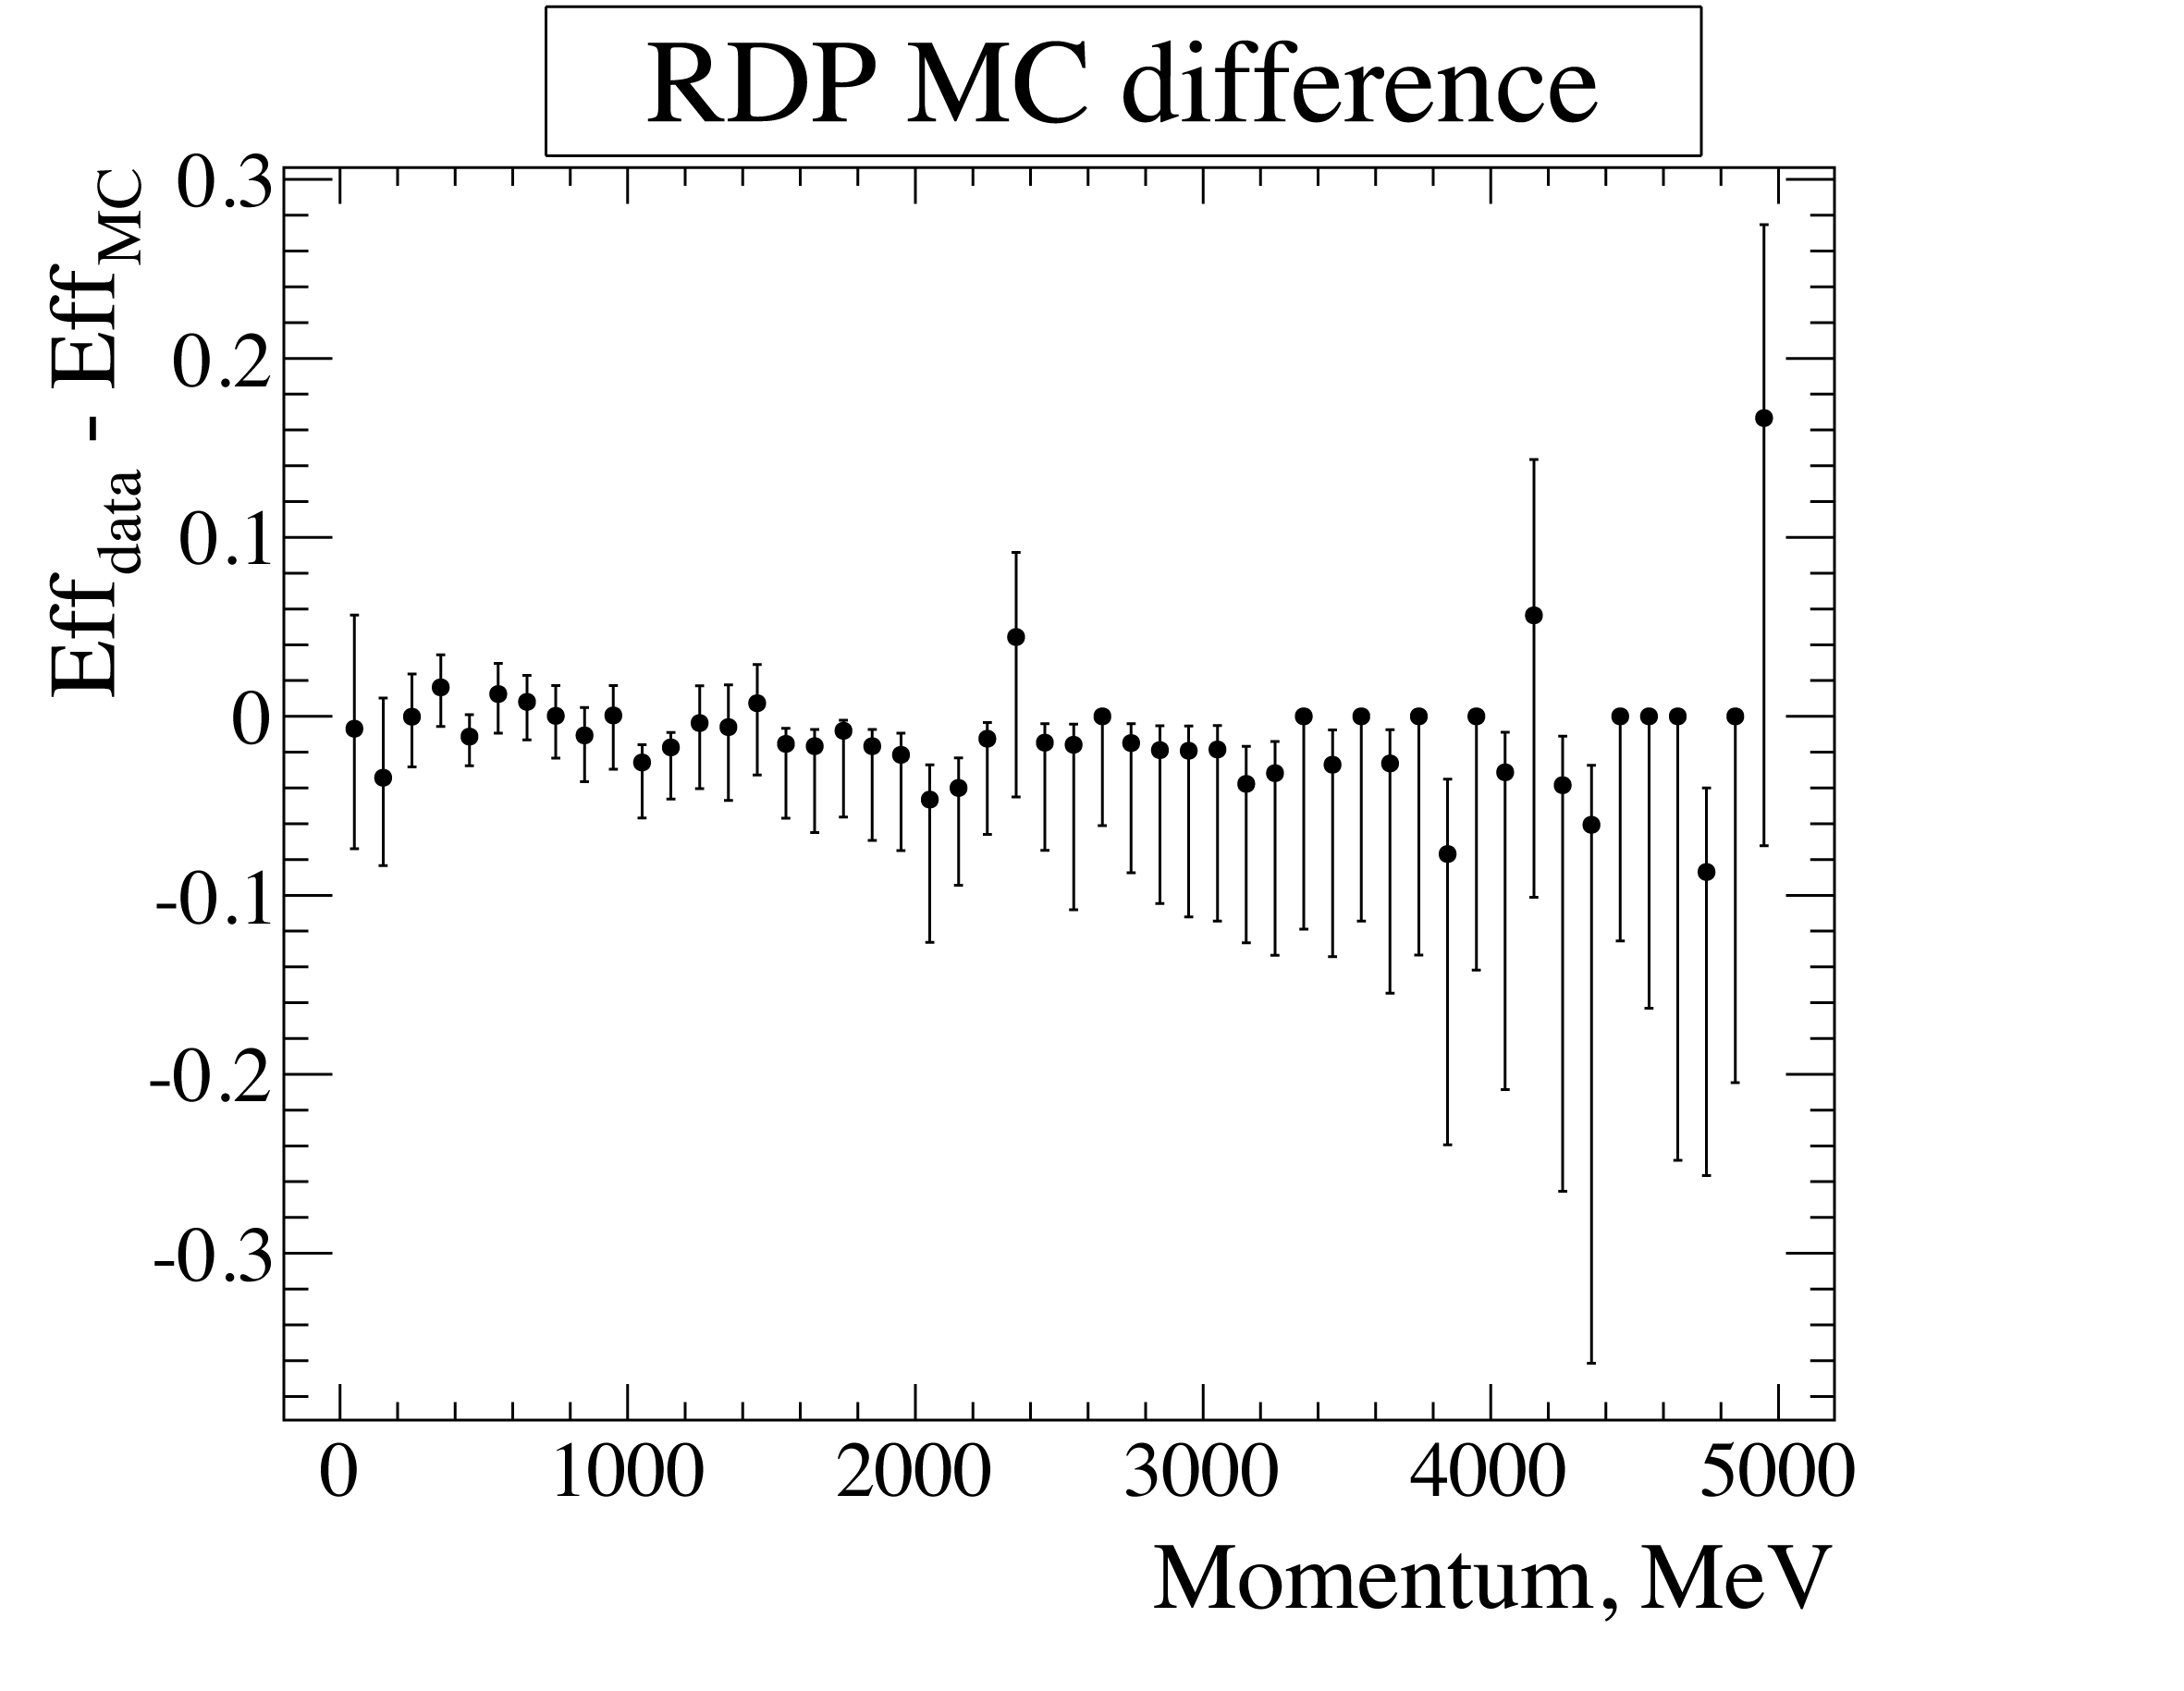
\includegraphics[width=\linewidth]{MomDifWide} \\ a)}
    \end{minipage}
    \hfill
    \begin{minipage}[h]{0.49\linewidth}
        \center{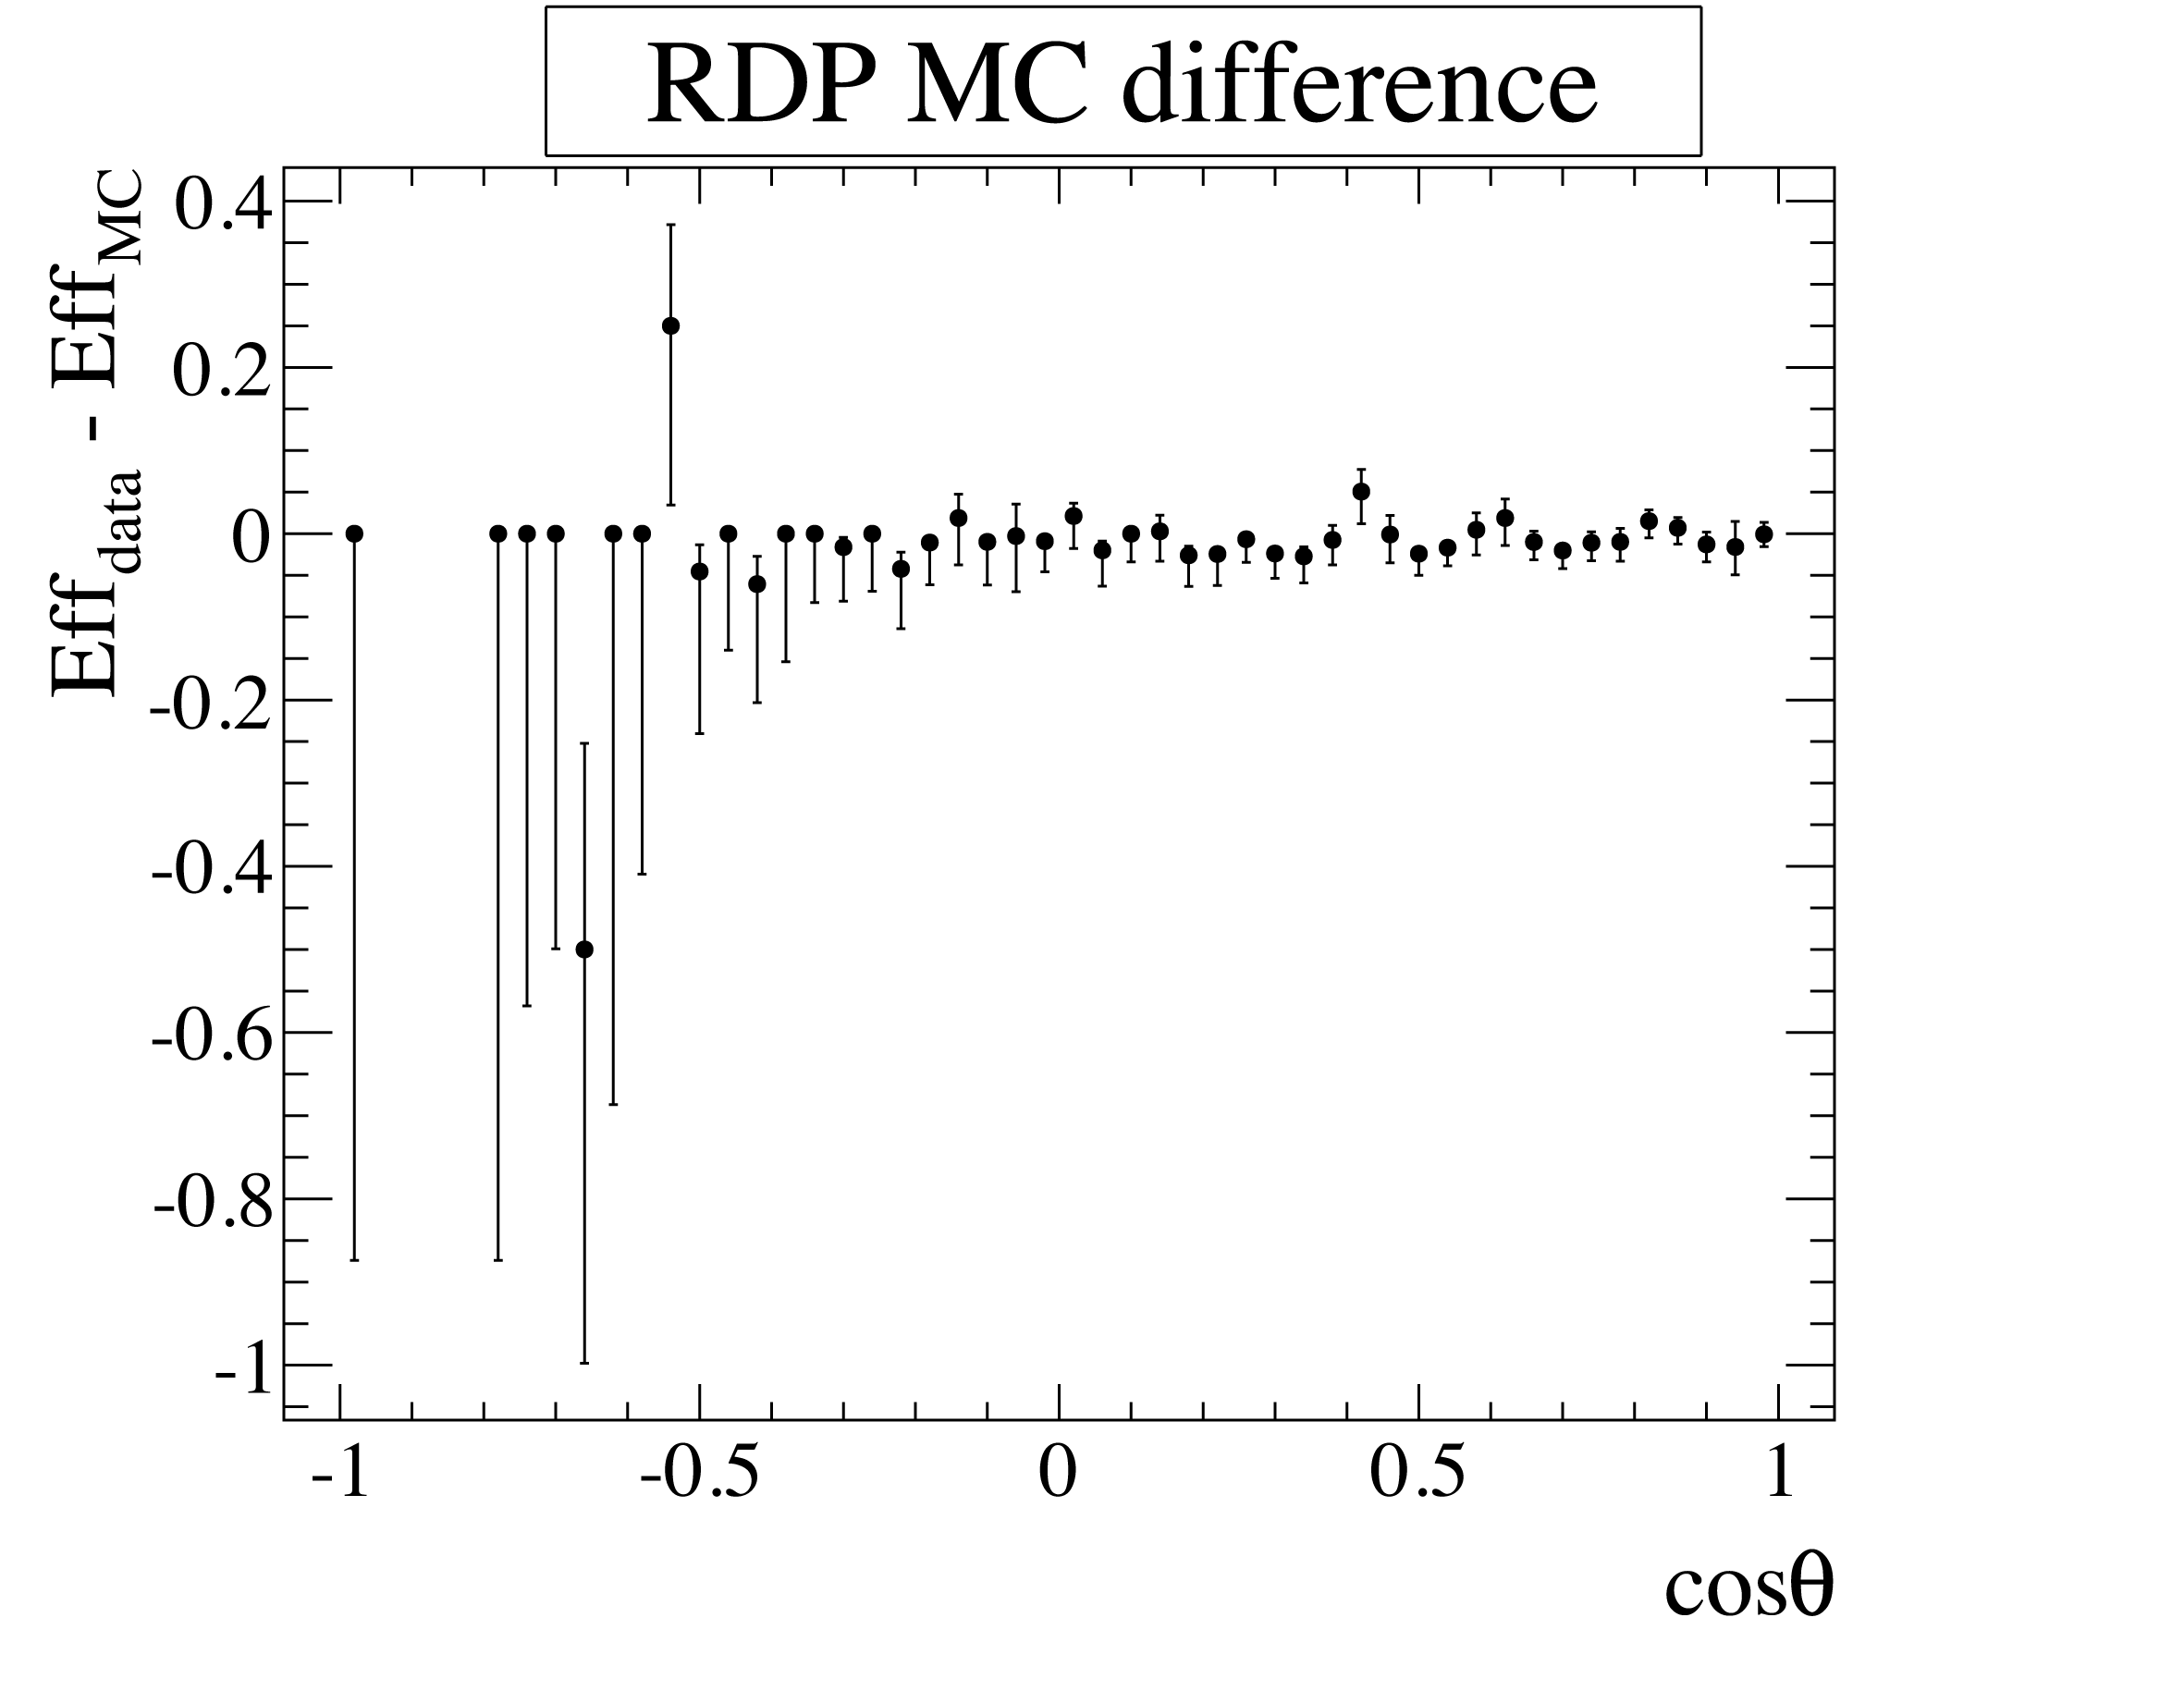
\includegraphics[width=\linewidth]{CosDifWide} \\ b)}
    \end{minipage}
    \caption{Dependence of the global vertex association systematics on the  track momentum (a) and on the opening angle (b) for FGD1 sample in black for DATA and in red for MC.}
    \label{fig:HNL:GVsysDEP}
\end{figure}

We conclude that there is neither angular nor momentum systematics dependence. The efficiency for MC and DATA are presented in~\autoref{tbl:HNL:GVsys}. The systematics for the HNL study was estimated using these efficiency differences with weight-like method.
\begin{table}[!ht]
\begin{center}
\begin{tabular}{|l|l|l|}
    \hline
    & FGD1 & FGD2 \\
    \hline
    DATA   & $0.958^{+0.0023}_{-0.0024}$ & $0.944^{+0.0027}_{-0.0026}$  \\
    \hline
    MC      & $0.962^{+0.0036}_{-0.0038}$ & $0.952^{+0.004}_{-0.0042}$  \\
    \hline
    Systematic uncertainty for $N\to\mu\pi$ & $0.58\%$ & $0.46\%$ \\
    \hline
    Systematic uncertainty for $N\to e\pi$ & $0.51\%$ & $0.4\%$ \\
    \hline

\end{tabular}
\caption{Global vertex association efficiency and systematics.}
\label{tbl:HNL:GVsys}
\end{center}
\end{table}
One more check is the spatial resolution comparison between the data and MC. We checked the difference between the track start position and the vertex position. The results are shown in~\autoref{fig:HNL:res}, the statistics is summarized in~\autoref{tbl:HNL:res}. As we can see the mean value for MC and data are rather close, the difference between them is near fit error and much less than RMS.
\begin{figure}[!ht]
\begin{center}
    \begin{minipage}{0.49\linewidth}
        \centering{\includegraphics[width=\linewidth]{ResolutionX}}
    \end{minipage}
    \hfill
    \begin{minipage}{0.49\linewidth}
        \centering{\includegraphics[width=\linewidth]{ResolutionY}}
    \end{minipage}
    \vfill
    \begin{minipage}{0.49\linewidth}
        \centering{\includegraphics[width=\linewidth]{ResolutionZ}}
    \end{minipage}
    \caption{Global vertex spatial resolution for experimental and MC data. Dots and left statistic box are experimental data, histograms and right statistic box is MC data.}
    \label{fig:HNL:res}
\end{center}
\end{figure}

\begin{table}[!ht]
\begin{center}
\begin{tabular}{|c|c|c|c|}
    \hline
    Axis & & Mean & RMS \\
    \hline
    \multirow{2}{*}{X} & MC & $0.16 \pm 0.09$ & $7.20\pm0.06$\\

    & DATA & $0.1\pm0.16$ & $7.67\pm0.11$ \\
    \hline
    \multirow{2}{*}{Y} & MC & $0.09 \pm 0.17$ & $8.29 \pm 0.12$\\

    & DATA & $0.14 \pm 0.09$ & $7.5 \pm 0.06$ \\
    \hline
    \multirow{2}{*}{Z} & MC & $-5.76 \pm 0.22$ & $10.68 \pm 0.15$\\

    & DATA & $-5.38 \pm 0.13$ & $10.78 \pm 0.09$ \\
    \hline
\end{tabular}
\caption{Summary of the statistics for spatial resolution for experimental and MC data presented in~\autoref{fig:HNL:res}.}
\label{tbl:HNL:res}
\end{center}
\end{table}

The global vertex systematics can be obtained only for the FGD but tracks from HNL decays start in TPC. So the following strategy was used: for the TPC1 tracks we consider systematics from the FGD1 sample, for the TPC2 and TPC3 tracks we apply the FGD2 sample results. This method gives the uncertainties at level $0.5\%$.

The results of all the systematic study are presented in~\autoref{tab:HNL:sys}.
\begin{table}[!ht]
\begin{center}
\begin{tabular}{|l |c| c| c|}
  \hline
   & $\mu\pi$ & $e\pi$ & $\mu\mu\nu$\\
  \hline
  \multicolumn{4}{||l|}{Variation-like} \\
  \hline
  B Field distortions                 & 0.48\%    & 0.37\%         &  0.02\%\\
  TPC momentum scale                  & 0.03\%    & 0.01\%         & 0.04\%\\
  TPC momentum resolution             & 2.34\%    & 0.78\%         & 0.46\%\\
  TPC PID                             & 0.41\%    & 0.75\%         & 1\%\\
  \hline
  \multicolumn{4}{||l|}{Efficiency-like} \\
  \hline
  TPC cluster efficiency              &   $\ll1\%$   &   $\ll1\%$  &  0.01\%\\
  TPC tracking efficiency             &   0.44\%     &  0.34 \%    & 0.46\% \\
  TPC charge ID efficiency            &   0.04\%     &   0.21\%    &   0.76\%\\
  TPC-FGD matching                    &   0.27\%     &    $\ll1\%$ & 0.03\%\\
  Pion secondary interactions         &   3.88\%     &   2.91\%    &  - \\
  Global vertex combining             &    0.58\%    &  0.52\%     & 0.48\%\\
  ECal PID                            &     -        &     -       & 0.27\%\\
  ECal TPC matching                   &     -        &     -       &  0.01\%\\
  \hline
  Total                               &   4.64\%     &  3.20\%     & 1.51\%\\
  \hline
\end{tabular}
\caption{Detector systematics summary.}
\label{tab:HNL:sys}
\end{center}
\end{table}

The systematic dependence on HNL mass is shown in~\autoref{fig:HNL:sys} and~\autoref{fig:HNL:sysDimuon}.

\begin{figure}[!ht]
  \begin{minipage}{0.49\linewidth}
    \centering{\includegraphics[width=\linewidth]{MuPiSys} \\ $K^+\to e^+N\to e^+\left(\mu^-\pi^+\right)$}
  \end{minipage}
  \begin{minipage}{0.49\linewidth}
    \centering{\includegraphics[width=\linewidth]{ElePiSys} \\ $K^+\to e^+N\to e^+\left(e^-\pi^+\right)$}
  \end{minipage}
  \caption{Detector systematics dependence on HNL mass}.
  \label{fig:HNL:sys}
\end{figure}

\begin{figure}[!ht]
    \centering{\includegraphics[width=0.49\linewidth]{DiMuonSys} \\ $K^+\to e^+N\to e^+\left(\mu^-\mu^+\nu\right)$}
  \caption{Detector systematics dependence on HNL mass}.
  \label{fig:HNL:sysDimuon}
\end{figure}


\subsection{Flux systematics}

Heavy neutrino flux in the ND280 is calculated based on the kaon flux in the decay volume (\autoref{ch:HNL:HNLsim}). Because of this, uncertainties in the kaon flux will affect the number of events. The total flux error consists of the meson multiplicities, pion rescatter, interaction length, focusing and other errors~\cite{Abe2013}. These fractional errors and the total flux uncertainty are presented on the Fig.~\ref{fig:HNL:FluxError}. In the the active neutrino studies the meson multiplicity uncertainty is dominated by the pion multiplicities. In our analysis we are sensitive only to kaon multiplicity errors. For the HNL analysis we consider all the uncertainties except meson multiplicities are the same as for the active neutrino flux. Thus to estimate kaon flux errors we take total neutrino flux error subtract meson multiplicity error and add kaon multiplicity uncertainty.

\begin{figure}[!ht]
  \centering{\includegraphics[width=0.49\linewidth]{NuFluxError.png} }
  \caption{$\nu_\mu$ Flux uncertainties.}
  \label{fig:HNL:FluxError}
\end{figure}

To estimate the kaon multiplicity errors we use data from NA61. Relative uncertainties on the K multiplicities are presented on the~\autoref{fig:HNL:KaonMult}. For HNL analysis we deal mainly with the kaons collinear to beam axis. We consider a conservative estimation of the kaon multiplicity uncertainty as 20\%. For all the other errors we take the maximum value among all energy bins -- 11\%.

\begin{figure}[!ht]
  \centering{\includegraphics[width=0.49\linewidth]{KaonError.png} }
  \caption{Kaon multiplicity uncertainties from TN-217.}
  \label{fig:HNL:KaonMult}
\end{figure}

The additional source of uncertainties is the flux reweight. For the HNL simulation we take so called ``nominal'' flux. It is the average neutrino flux. The real flux changes a bit from run to run. The run change is realized with the help of the renormalization of the event weight for every run. We used the reweight files and checked that the run differences affect on our result in order $\ll1\%$. The error from this effect was summarized in quadrature with all other flux errors.

The results of the systematics study are presented on the~\autoref{fig:HNL:AllSys}. The detector systematics is widely described in previous subsection. As we analyze all charge conjugated modes together we take the highest systematics uncertainties among them.

\begin{figure}[!ht]
    \begin{center}
    \begin{minipage}{0.49\linewidth}
        \centering{\includegraphics[width=\linewidth]{FluxMu}  \\  $N\to\mu\pi$}
    \end{minipage}
    \hfill
    \begin{minipage}{0.49\linewidth}
        \centering{\includegraphics[width=\linewidth]{FluxEle}  \\  $N\to e\pi$}
    \end{minipage}
    \vfill
    \begin{minipage}{0.49\linewidth}
        \centering{\includegraphics[width=\linewidth]{FluxDiMu}  \\  $N\to\mu\mu\nu$}
    \end{minipage}
    \caption{Detector and flux systematic errors for different modes.}
    \label{fig:HNL:AllSys}
        \end{center}
\end{figure}



\subsection{Pile up}
\label{sec:HNL:pileup}
For the veto cuts we look for the activity in the upstream detector. Also we reject the events that have tracks in the TPC with HNL candidate that doesn't correspond to the HNL daughters. These are possible sources for the pile ups. The percentages of such events in the real data are summarized in~\autoref{tbl:HNL:pileUp}. In the table we use symbol ``A'' to mark the run period when P0D was filled with air and ``W'' when it was filled with water. The content of the P0D may have influence on the result of applying our veto cut. We have studied both $\nu$ and $\bar{\nu}$ runs as the pile ups can be different for them. Also the two main sources of pile ups are separated for each TPC. For the correction we use the maximum pile up value from all the runs in the each TPC which is shown in red. In fact with this method effect of the pileups is overestimated.
\begin{table}
\begin{center}
\begin{tabular}{|l|c|c|c|c|c|}
  \hline
  Cut         &Run 1W   &Run 2W   & Run 2A  & Run 3b A&Run 3c A\\
  \hline
  TPC1 start  & 0.3\%   & 0.61\%  & 0.69\%  & 0.64\%  & 0.75\%  \\
  TPC1 veto   & 0.32\%  & 0.43\%  & 0.49\%  & 1.83\%  & 2.15\%  \\
  TPC1 all    & 0.57\%  & 0.96\%  & 1.00\%  & 1.08\%  & 2.75\%   \\
  \hline
  TPC2 start  & 0.25\%  & 0.48\%  & 0.55\%  & 0.52\%  & 0.6\%  \\
  TPC2 veto   & 1.03\%  & 1.73\%  & 2\%     & 1.83\%  & 2.18\% \\
  TPC2 all    & 1.19\%  & 2.05\%  & 2.36\%  & 2.18\%  & 2.57\%  \\
  \hline
  TPC3 start  & 0.26\%  & 0.46\%  & 0.53\%  & 0.48\%  & 0.57\%  \\
  TPC3 veto   & 0.93\%  & 1.56\%  & 1.78\%  & 1.64\%  & 1.95\%  \\
  TPC3 all    & 1.1\%   & 1.85\%  & 2.11\%  & 1.95\%  & 2.3\%  \\
  \hline
  \hline
              &Run 4W   &Run 4A   &Run 5W   &Run 5W$\bar{\nu}$  &Run 6A$\bar{\nu}$\\
  \hline
  TPC1 start  & 0.89\%  & 0.95\% & 0.7\% & 0.35\% & 0.45\% \\
  TPC1 veto   & 2.55\%  & 2.76\% & 1.95\% & 0.96\% & 1.26\% \\
  TPC1 all    & 3.25\%  &\textcolor{red}{3.45\%} & 2.51\% & 1.25\% & 1.62\% \\
  \hline
  TPC2 start  & 0.71\%  & 0.76\% & 0.55\% & 0.29\% & 0.38\% \\
  TPC2 veto   & 2.65\%  & 2.76\% & 2.03\% & 1.15\% & 1.47\% \\
  TPC2 all    & 3.1\%   & 3.24\% & 2.39\% & 1.34\% & 1.71\% \\
  \hline
  TPC3 start  & 0.68\%  & 0.72\% & 0.53\% & 0.28\% & 0.35\% \\
  TPC3 veto   & 2.34\%  & 2.46\% & 1.81\% & 1.02\% & 1.31\% \\
  TPC3 all    & 2.75\%  & 2.89\% & 2.15\% & 1.2\% & 1.54\% \\
  \hline
  \hline
              &Run 7b   &Run 7c   &Run 8A   &Run 8A  & \\
  \hline
  TPC1 start  & 0.62\%  & 1.74\% & 1.76\% & 1.27\% & \\
  TPC1 veto   & 0.55\%  & 1.46\% & 1.26\% & 0.93\% &  \\
  TPC1 all    & 1.07\%  & 2.93\% & 2.77\% & 2.02\% & \\
  \hline
  TPC2 start  & 0.52\%  & 2.30\% & 1.37\% & 0.99\% & \\
  TPC2 veto   & 2.03\%  & 4.73\% & 4.63\% & 3.42\% &  \\
  TPC2 all    & 2.35\%  & \textcolor{red}{5.53\%} & 5.43\% & 2.83\% &\\
  \hline
  TPC3 start  & 0.49\%  & 1.30\% & 1.33\% & 0.96\% & \\
  TPC3 veto   & 1.81\%  & 4.23\% & 4.14\% & 3.06\% &  \\
  TPC3 all    & 2.11\%  & \textcolor{red}{4.94\%} & 4.84\% & 3.57\% &  \\
  \hline
\end{tabular}
\caption{Event pile up in real data.}
\label{tbl:HNL:pileUp}
\end{center}
\end{table}


\section{Statistical methods}
\label{sec:HNL:stat}
The statistical approach to the low level signal analysis is described in the Highland and Cousins work~\cite{Cousins1992}. As number of the HNL decay events is proportional to the forth power of the mixing element (\autoref{ch:HNL:HNLsim}), constraints on $\left|U_i\right|^2$ without systematics looks like:
\begin{equation}
  \left|U_i\right|^2_{limit}=\sqrt{\frac{U_n}{N_{events}}}
  \label{eq:HNL:constraints}
\end{equation}
where $i=e,\mu$, $U_n$ is 90\% C.L. Poisson limit for $n$ observed events and $N_{events}$ is expected number of signal events assuming $\left|U\right|^2=1$. If we take into account the detector acceptance uncertainty, the result can be calculated according to~\cite{Cousins1992}:
\begin{equation}
  U_n=U_{n0}\left\{1+E_n\frac{\sigma^2_{Acc}}{2}\left(1+\left(\frac{E_n\sigma_{Acc}}{2}\right)^2\right)\right\}
  \label{eq:HNL:constrainsAcc}
\end{equation}
where $U_{n0}$ is 90\% C.L. Poisson limit for $n$ observed events, $\sigma_{Acc}$ is the acceptance error, $E_n=U_{n0}-n$ represents the excess of the upper limit of a Poisson parameter over the number n of observed events, for a specified confidence level. This approach can be applied only while $\sigma_{Acc}<1/E_n$. We will show that in our study $\sigma_{Acc}\approx0.3$ and $1/E_n>0.5$ (this values are described in the section~\ref{sec:HNL:sys}). So this method can be applied for the analysis.


\chapter{Results}
\section{MC sensitivity estimations}
\label{sec:HNL:MCres}

After studying the MC efficiency (\autoref{sec:HNL:eff}), background processes (\autoref{sec:HNL:bg}), systematics (\autoref{sec:HNL:sys}) and pile ups (\autoref{sec:HNL:pileup}),  sensitivity to the mixing elements based on MC could be estimated according to~\autoref{eq:HNL:constrainsAcc}). The results are shown in~\autoref{fig:HNL:LimitsMC1} and~\autoref{fig:HNL:LimitsMC2}. Because of the small background the acceptance uncertainties have a small effect on the sensitivity.

\begin{figure}[!ht]
    \begin{center}
  \begin{minipage}{0.49\linewidth}
    \centering{\includegraphics[width=\linewidth]{Ue2fullMC}  \\  $K^+\to e(e\pi)$}
  \end{minipage}
  \hfill
  \begin{minipage}{0.49\linewidth}
    \centering{\includegraphics[width=\linewidth]{Umu2fullMC}  \\  $K^+\to \mu(\mu\pi)$}
  \end{minipage}
  \caption{Sensitivity to mixing elements $\left|Ue\right|^2, \left|U\mu\right|^2$ based on MC samples analysis}
  \label{fig:HNL:LimitsMC1}
    \end{center}
\end{figure}

\begin{figure}[!ht]
    \begin{center}
  \begin{minipage}{0.49\linewidth}
    \centering{\includegraphics[width=\linewidth]{UeUmufullMC}  \\  $K^+\to \mu(e\pi)$ and $K^+\to e(\mu\pi)$}
  \end{minipage}
  \begin{minipage}{0.49\linewidth}
    \centering{\includegraphics[width=\linewidth]{UeMixfullMC}  \\  $K^+\to e(\mu\mu\nu)$}
  \end{minipage}
  \caption{Sensitivity to mixing elements $\left|UeU\mu\right|$ and $\left|U_{e}\right|\sqrt{\left|U_{e}\right|^2+\left|U_{\tau}\right|^2}$ based on MC samples analysis.}
  \label{fig:HNL:LimitsMC2}
  \end{center}
\end{figure}

As one can see the improvements of PS191 limits can be obtained with the current statistics.

\section{Data unblinding}
The current analysis was approved for the data unblinding. The numbers of observed events in data are presented in the~\autoref{tbl:HNL:Ndata}. As mentioned above (\autoref{sec:HNL:bg}) run 8 data samples are available only for the preliminary analysis. So all the results are presented for full ND280 data set (run 2-8).

\begin{table}[!ht]
\begin{center}
\begin{tabular}{llll}
                            & Events in data      \\
  $\mu\pi$ \hspace{0.5cm}   & 0  \hspace{2cm}     \\
  $e\pi$                    & 0                   \\
  $\mu\mu\nu$               & 1                   \\
\end{tabular}
\caption{The total number of events observed in data.}
\label{tbl:HNL:Ndata}
\end{center}
\end{table}

One event for the $N\to\mu\mu\nu$ mode was observed. It happened in the TPC3 and looks like the signal event: two muon-like tracks with the direction extremely collinear to beam axis. The event display for this event is presented in~\autoref{fig:HNL:DataEvent}.

\begin{figure}[!ht]
    \begin{center}
  \begin{minipage}{0.49\linewidth}
    \centering{\includegraphics[width=\linewidth]{DataEvent2}}
  \end{minipage}
  \begin{minipage}{0.49\linewidth}
    \centering{\includegraphics[width=\linewidth]{DataEvent1}}
  \end{minipage}
  \caption{Event observed in the $N\to\mu\mu\nu$ mode in the data sample in the TPC3.}
  \label{fig:HNL:DataEvent}
  \end{center}
\end{figure}

More accurate study shows that the invariant mass of this muon pair is too high for the heavy neutrino decay $M_{inv}\approx$ GeV. But based on blind analysis method and our analysis strategy this event will be treated as a signal and appropriate upper limit on the mining element will be set.

Based on this numbers final sensitivity to mixing elements based on our analysis can be estimated. The results are presented in~\autoref{fig:HNL:LimitsData1} and~\autoref{fig:HNL:LimitsData2}.

\begin{figure}[!ht]
    \begin{center}
  \begin{minipage}{0.49\linewidth}
    \centering{\includegraphics[width=\linewidth]{Ue2fullDATA}  \\  $K^+\to e(e\pi)$}
  \end{minipage}
  \hfill
  \begin{minipage}{0.49\linewidth}
    \centering{\includegraphics[width=\linewidth]{Umu2fullDATA}  \\  $K^+\to \mu(\mu\pi)$}
  \end{minipage}
  \caption{Sensitivity to mixing elements $\left|Ue\right|^2, \left|U\mu\right|^2$ based on the data samples analysis.}
  \label{fig:HNL:LimitsData1}
    \end{center}
\end{figure}

\begin{figure}[!ht]
    \begin{center}
  \begin{minipage}{0.49\linewidth}
    \centering{\includegraphics[width=\linewidth]{UeUmufullDATA}  \\  $K^+\to \mu(e\pi)$ and $K^+\to e(\mu\pi)$}
  \end{minipage}
  \begin{minipage}{0.49\linewidth}
    \centering{\includegraphics[width=\linewidth]{UeMixfullDATA}  \\  $K^+\to e(\mu\mu\nu)$}
  \end{minipage}
  \caption{Sensitivity to mixing elements $\left|UeU\mu\right|$ and $\left|U_{e}\right|\sqrt{\left|U_{e}\right|^2+\left|U_{\tau}\right|^2}$ based on the data samples analysis.}
  \label{fig:HNL:LimitsData2}
  \end{center}
\end{figure}

\section{Prospects}
\end{document}